% This is LLNCS.DEM the demonstration file of
% the LaTeX macro package from Springer-Verlag
% for Lecture Notes in Computer Science,
% version 2.4 for LaTeX2e as of 16. April 2010
%
\documentclass[10pt, a4paper]{article}
%
\usepackage{makeidx}  % allows for indexgeneration
%

% allow for compress references ranges
% noadjust removes a leading space before the []
\usepackage[noadjust]{cite}


\usepackage[english,activeacute]{babel}
\usepackage[english]{layout}
\usepackage{amsfonts,amssymb}
\usepackage[cmex10]{amsmath}
\usepackage{amsopn} % DeclareMathOperator
\usepackage{amsbsy} % boldsymbol
\usepackage[dvips]{graphicx}
\usepackage{color}
\usepackage{subfig}
\usepackage{colonequals}
\usepackage[latin1]{inputenc}
\usepackage{url}
\usepackage{epsfig}
\usepackage{dsfont}
\usepackage{multirow}

\usepackage{algorithm}
\usepackage{algorithmic}
\usepackage{setspace}
\usepackage{afterpage}
%\usepackage{showkeys}
% \usepackage{mathptmx}      % use Times fonts if available on your TeX system
% \usepackage{latexsym}

\usepackage[left=1.0in,right=1.0in]{geometry}
\usepackage{pdflscape}
\usepackage{hyperref}

\usepackage[normalem]{ulem} % allows the use of sout

% \graphicspath{{../iccv09/}}

% pablo's commands for comments and suggested modifications
%\newcommand{\pa}[1]{\textcolor{cyan}{#1}}
\newcommand{\pa}[1]{#1}
\newcommand{\psub}[2]{\pa{\sout{#1}}\pa{/#2}}
\newcommand{\prm}[1]{\pa{\sout{#1}}}
\newcommand{\padd}[1]{\pa{#1}}
%\newcommand{\pcomment}[1]{\textit{\pa{#1}}}
\newcommand{\pcomment}[1]{}

%\newcommand{\best}[1]{\textbf{\textcolor{MyOrange}{#1}}}
\newcommand{\best}[1]{#1}
\newcommand{\bsic}[1]{\textcolor{black}{\textit{#1}}}
\newcommand{\Bsic}[1]{\textcolor{black}{\textbf{\textit{#1}}}}
\newcommand{\Best}[1]{\textbf{\textcolor{black}{#1}}}

\newcommand{\ma}[1]{\boldsymbol{#1}}
\newcommand{\tras}[1]{#1^{\mathrm{T}}}
\newcommand{\herm}[1]{#1^{\mathrm{H}}}
\newcommand{\con}[1]{#1^{\mathrm{*}}}
\newcommand{\E}{\mathds{E}}
\newcommand{\tech}[1]{\overline{#1}}
\newcommand{\nspace}{\!\!\!\!}
\newcommand{\nmbr}[1]{\oldstylenums{#1}}

\newcommand{\eg}{\emph{e.g}. } \newcommand{\Eg}{\emph{E.g}. }
\newcommand{\ie}{\emph{i.e}. } \newcommand{\Ie}{\emph{I.e}. }
\newcommand{\cf}{\emph{c.f}. } \newcommand{\Cf}{\emph{C.f}. }
\newcommand{\etc}{\emph{etc}. } \newcommand{\vs}{\emph{vs}. }
\newcommand{\wrt}{w.r.t\onedot } \newcommand{\dof}{d.o.f. }
\newcommand{\etal}{\emph{et al}. }

\newcommand{\R}{\mathds{R}}
\newcommand{\sign}{\mathrm{sign}}
\newcommand{\eps}{\varepsilon}
\newcommand{\To}{\longrightarrow}
% \newcommand{\II}{1{\hskip -2.5 pt}\hbox{I}}

\renewcommand{\algorithmiccomment}[1]{\bgroup\hfill\small\textcolor{gray}{//~#1}\egroup}

% c++ code
\usepackage{listings}
\usepackage{xcolor}
\usepackage{textcomp}
\definecolor{listinggray}{gray}{0.9}
\definecolor{lbcolor}{rgb}{0.9,0.9,0.9}
\lstset{
	backgroundcolor=\color{lbcolor},
	tabsize=4,    
%  rulecolor=,
	language=Matlab,
	basicstyle=\scriptsize\ttfamily,
	upquote=true,
	aboveskip={1.5\baselineskip},
	columns=fixed,
	showstringspaces=false,
	extendedchars=false,
	breaklines=true,
	prebreak = \raisebox{0ex}[0ex][0ex]{\ensuremath{\hookleftarrow}},
	frame=single,
	numbers=left,
	showtabs=false,
	showspaces=false,
	showstringspaces=false,
	identifierstyle=\ttfamily,
	keywordstyle=\color[rgb]{0,0,1}\ttfamily,
	commentstyle=\color[rgb]{0,0.5,0}\ttfamily,
	stringstyle=\color[rgb]{0.627,0.126,0.941}\ttfamily,
	numberstyle=\color[rgb]{0.5, 0.5, 0.5}\ttfamily,
%  \lstdefinestyle{C++}{language=C++,style=numbers}’.
}
%\lstset{
%	backgroundcolor=\color{lbcolor},
%	tabsize=4,
%	language=C++,
%	captionpos=b,
%	tabsize=3,
%	frame=lines,
%	numbers=left,
%	numberstyle=\tiny,
%	numbersep=5pt,
%	breaklines=true,
%	showstringspaces=false,
%	basicstyle=\footnotesize,
%	identifierstyle=\color{magenta},
%	keywordstyle=\color[rgb]{0,0,1},
%	commentstyle=\color{green},
%	stringstyle=\color{red}
%}
	
	
	


\DeclareMathOperator*{\argmin}{arg\,min}
\DeclareMathOperator*{\argmax}{arg\,max}

\newcommand{\nota}[1]{\textcolor{blue}{\textbf{#1}}}
\newcommand{\suggest}[1]{\textcolor{cyan}{#1}}
\newcommand{\add}[1]{\textcolor{green}{#1}}
\newcommand{\remove}[1]{\textcolor{red}{#1}}
\newcommand{\todo}[1]{\textcolor{red}{\noindent\textsc{todo}: #1}}
\newcommand{\dosdv}[1] {#1}
\newcommand{\uncite}[1] {}
% \newcommand{\tachar}[1]{
% \setbox4=\hbox{\ } \setbox3=\hbox{#1} \hbox{#1} \kern -\wd3 \kern
% -\wd4 \raise 0.3\ht3 \hbox{ \vrule width \wd3 height 0.5pt} }

% \theoremstyle{plain}\newtheorem{theorem}{Theorem}[chapter]
% \theoremstyle{plain}\newtheorem{proposition}{Proposition}[chapter]
% \theoremstyle{plain}\newtheorem{lemma}{Lemma}[chapter]
% \theoremstyle{definition}\newtheorem{definition}{Definition}[chapter]

%% % New definition of square root:
%% % it renames \sqrt as \oldsqrt
%% \let\oldsqrt\sqrt
%% % it defines the new \sqrt in terms of the old one
%% \def\sqrt{\mathpalette\DHLhksqrt}
%% \def\DHLhksqrt#1#2{%
%% \setbox0=\hbox{$#1\oldsqrt{#2\,}$}\dimen0=\ht0
%% \advance\dimen0-0.2\ht0
%% \setbox2=\hbox{\vrule height\ht0 depth -\dimen0}%
%% {\box0\lower0.4pt\box2}}

\title{A Non-local Bayesian Video Denoising Method}
\date{}

\author{Pablo~Arias, Jean-Michel~Morel%
\thanks{P. Arias (\texttt{pablo.arias@cmla.ens-cachan.fr}) and J.-M. Morel
(\texttt{jean-michel.morel@cmla.ens-cachan.fr}) are with the \emph{Centre de
math\'ematiques et de leurs applications} (CMLA), \'Ecole Normale Sup\'eriore
de Cachan, 61 Av. du Pr\'esident Wilson, F-94230 Cachan, France}
\\[1ex] CMLA, ENS Cachan}


\makeatletter         
\def\@maketitle{
\raggedright
\begin{center}
	{\huge \bfseries \sffamily \@title }\\[8ex] 
	{\Large \bfseries \sffamily Report for the Project }\\
	
\includegraphics[width = 80mm]{Plein-Phare.png}\\[8ex]
	{\Large  \@author}\\[4ex] 
\end{center}}
\makeatother


\begin{document}



\maketitle              % typeset the title of the contribution

\begin{abstract}
	The quality provided by image/video sensors increases steadily, and
	for a fixed spatial resolution the sensor noise has been gradually reduced.
	However, modern sensors are also capable of acquiring at higher spatial
	resolutions which are still affected by noise, specially at low lighting
	conditions. The situation is even worse in video cameras, where the capture
	time is bounded by the frame rate. The noise in the video degrades its visual 
	quality and hinders its analysis.
	In this paper we present a new video denoising method extending 
	the non-local Bayes image denoising algorithm. The method does not require 
	motion estimation, and yet preliminary results show that it outperforms the
	state-of-the-art methods in terms of PSNR.
\end{abstract}

%
\section{Introduction}
%

Advances in video sensor hardware have steadily improved the acquisition
quality. However, due to the reduction in the price of cameras
and data storage, video cameras are being used more each time, and in less
favorable situations, such as low lighting conditions. This results in high 
levels of noise, which negatively affects the visual quality of the video and
hinders its use for any application. 
\pcomment{It would be nice to have some reference for these claims about
sensors, camera prices, etc.}

Video denoising has received much less attention than still image denoising in
the literature.  In principle, denoising videos should be easier than still
images, since the strong temporal redundancy along motion trajectories favours
the denoising task. However, this additional form of redundancy creates
challenges.  On one hand, the amount of data is much larger than for still
images, and efficient ways of navigating through this data are needed. On the
other hand, the output of the denoising algorithm should be temporally
consistent according to the motion of the original sequence.

Early works proposed temporal or spatio-temporal filters which either compensate
for motion on estimated motion trajectories or used some kind of mechanism to
adapt to the changes in the video signal at a fixed location due to the motion.
We refer the reader to \cite{Brailean1995a} and references therein for more details.
Other video denoising works apply temporal filtering to the wavelet coefficients 
of the frames \cite{Jin2006,Zlokolica2006a}. 

Some methods do not distinguish between the temporal and spatial dimensions,
and treat the video as a volume, which is denoised in a transformed domain
\cite{Rajpoot2003,Wilson2004,Selesnick2003}. 
\pcomment{TODO: Read these references. Even if they consider a 3D transform, I think
they DO distinguish between space and time}

Until the advent of patch-based approaches, methods without motion compensation
failed in the presence of moderate motion, and their main interest resided
in their simplicity and low computational cost. First state-of-the-art results
obtained without motion estimation were reported in \cite{Buades2005v}, with the
non-local means algorithm. The authors argued that for their method, based on
averaging similar patches, motion estimation was not only unnecessary but
counterproductive: while textured regions are problematic for motion
estimation, they are a source of a large number of similar patches across
different frames. Even if the motion trajectory could be reliably estimated, it
makes more sense to use all similar patches, rather than using only the ones on the
trajectory.
%
A similar approach was followed by the authors of \cite{Dabov2007v}. This method is based
on collaborative filtering of similar patches in a
spatio-temporal neighborhood. 

The methods in \cite{Buades2005v} and \cite{Dabov2007v} are extensions to video
of still image patch-based denoising algorithms (non-local means \cite{Buades2006} and BM3D
\cite{Dabov2007tip} respectively). They are based on filtering similar 2D patches
searched for in a 3D spatio-temporal neighborhood. These methods exploit both
spatial and temporal redundancy, however, since each 2D patch is processed
independently, there is no mechanism to impose coherence along trajectories.
This results in flickering artifacts which become noticeable for high levels of
noise. 
%
While these methods exploit spatio-temporal redundancy, they do not impose
coherence of the trajectories, resulting in flickering
artifacts which become noticeable for high levels of noise. 

An interesting alternative was proposed in \cite{Liu2010},
based on non-local means.
To denoise a target 2D patch in a frame, its forward and backward trajectories are
determined using a robust optical flow algorithm based on \cite{Bruhn2005}. 
Each half of the trajectory extends for $t$ frames. There are $2t + 1$ 2D patches
centered at each point of the trajectory.
For each of these patches, the $n$ nearest neighbors are found
using an efficient approximate searching strategy. The target 2D patch is denoised
by performing a weighted average of these $(2t + 1)n$ patches. The weight considers
the patch similarity as in the original non-local means method, multiplied by a coefficient
that decreases smoothly with the temporal distance between a source patch and the target patch.
%
In this way, 2D patches in the same trajectory are denoised using a smoothly
varying non-local average of similar 2D patches. The result is a video with
a high temporal consistency.

A natural next step is to consider 3D spatio-temporal patches. This has two
main advantages (at the expense of a higher computational cost). First it
provides a mechanism to impose some temporal consistency on the result, since
now, the temporally contiguous 2D spatial slices of a spatio-temporal patch
are filtered jointly. Secondly, a 3D patch has a higher number of pixels
resulting in a reduction of the noise in the distance between patches. On the
other hand, to get the same reduction in the distance noise with 2D patches one
needs to increase their spatial size which leads to a smaller number of similar
patches.

Two types of 3D patches have been used: rectangular and motion-compensated.
Motion-compensated 3D patches follow a motion trajectory previously estimated.
Each approach has its pros and cons.

Motion-compensated patches have the benefit that their spatial slices are very
similar between each other. As a consequence, temporal filtering can be easily performed by
filtering inside the patch in the temporal direction. 
Because of this, methods that use motion-compensated 3D patches only look for
similar motion-compensated 3D patches starting in the same frame.


In \cite{Maggioni2011,Maggioni2012}, the authors introduced V-BM4D, an
extension of BM3D to video by collaborative filtering of similar motion
compensated 3D patches. Trajectories are computed with a block matching
strategy based on the sum of squared differences (SSD) and a temporal
regularization term, which favours trajectories with small velocity and low
acceleration. The results of this algorithm show higher PSNR and temporal
consistency, resulting in a higher overall quality.

One of the main difficulties in using motion-compensated patches is estimating
motion. Motion estimation is a paramount problem in noiseless sequences, and
noise makes it much harder.

Rectangular 3D patches offer an appealing
alternative, since they do not require estimating motion. 
In \cite{Protter2007,Protter2009} the authors extend the K-SVD \cite{Elad2006}
image denoising method to video by learning a dictionary of spatio-temporal
rectangular 3D patches.

Each rectangular 3D patch results from the combination of a 2D texture and a
motion pattern. For arbitrary motion, each combination of texture and motion is
not likely to occur together again. Thus rectangular 3D patches should have
less repeatability in the video compared to motion compensated patches.  An
exception is when the motion is a global translation of the frame, in which
case, the motion pattern is equal for each patch. Furthermore, if there is no
acceleration (uniform motion), rectangular 3D patches are constant along motion
trajectories. Global uniform motion is indeed a too restrictive model, but in
many cases, it is a valid approximation in a local neighborhood in space and
time.

\bigskip

In this work we present new Bayesian patch-based video denoising method using
3D rectangular patches and not requiring motion estimation.
Yet, it provides
results which compare favourably to the current state-of-the-art,
both quantitatively by a significant margin and qualitatively, specifically in
terms of the temporal consistency attained.
In the spirit of  \cite{Lebrun2013a,Lebrun2013ipol},
the method works by learning a Gaussian \emph{a priori} model from sets of 
similar noisy patches. Each patch is denoised by computing the \emph{maximum a
posteriori} (MAP) with the estimated prior.
Learning the Gaussian prior amounts to estimating a covariance matrix with a
limited number of samples in a high dimensional space. Motivated by recent 
theoretical results and supported by an empirical analysis, we add the 
assumption that the \emph{a priori} model is of low rank (\ie the clean patches
lie in a lower dimensional subspace). This assumption lowers the computational cost
of the algorithm, and improves the results.



\bigskip

The rest of the paper is organized as follows: in \S
\ref{sec:review_nonlocal_Bayes} we review our patch-based Bayesian optimal estimator for
video denoising. The final algorithm and details about its implementation are
given in \S \ref{sec:algorithm}.
Some relevant aspects of the proposed method are discussed in \S
\ref{sec:discussion}.
In \S \ref{sec:parameters}
we explain the selection of the parameters. Some results, including a
comparison with the state-of-the-art methods, are shown in \S
\ref{sec:results}. Concluding remarks are given in \S \ref{sec:conclusion}.

\section{Bayesian video denoising}
\label{sec:review_nonlocal_Bayes}

Our fundamental assumption is that video patches similar to a given
patch follow a Gaussian distribution.
The problem 
of denoising can then be formulated as a problem of optimal Bayesian inference, where the
parameters of the prior are learnt from the noisy data.

%Consider a grayscale video $u:\Omega\times \{1,\cdots,T\}\rightarrow
%\mathbb R$, where $\Omega$ is the spatial domain (a rectangular discrete grid).
%We assume that $v$ is a noisy version of $u$, contaminated with additive,
%Gaussian, white noise $n$ of known variance $\sigma^2$,
%\[v = u + n.\]
%
%We make the assumption that each patch $\ma p_{xt}$ of the noiseless video is a realisation 
%of a Gaussian random variable, $N(\overline {\ma p}_{xt}, C_{xt})$.
%%
%The problem 
%of denoising can then be formulated as a problem of optimal Bayesian inference, where the
%parameters of the prior are learnt from the noisy data.
%%
%If the
%mean and covariance are known (or leant from the data), then given a noisy observation
%$\ma q_{xt} = \ma p_{xt} + \ma n_{xt}$, 
%one can estimate $\ma p_{xt}$ as the expected value of the posterior
%distribution $\mathds{P}(\ma p_{xt}, \ma q_{xt})$ or its
%maximum (\ie the maximum \emph{a posteriori}, MAP).



\subsection{A nonlocal Bayesian principle}

Consider a grayscale video $u:\Omega\times \{1,\cdots,T\}\rightarrow
\mathbb R$, where $\Omega$ is the spatial domain (a rectangular discrete grid).
We assume that $v$ is a noisy version of $u$, contaminated with additive,
Gaussian, white noise $n$ of known variance $\sigma^2$,
\[v = u + n.\]

Given a rectangular 3D patch $\ma q$ of size $s_x\times s_x\times s_t$ of the noisy video $v$, and the 
corresponding patch $\ma p$ of the clean video $u$, we assume the following 
Gaussian linear model of $\ma p$ and $\ma q$:
\begin{align}
	\mathds{P}(\ma p) &= \mathcal N(\overline {\ma p}, C) \propto \exp\left(-\frac12\langle \ma p - \overline{\ma p}, C^{-1}(\ma p - \overline{\ma p})\rangle\right) \label{eq:prior}\\
	\mathds{P}(\ma q|\ma p) &= \mathcal N(\ma p, \sigma I) \propto \exp\left(-\frac1{2\sigma^2}\|\ma q - \ma p\|^2\right) \label{eq:obs}
\end{align}
Once the mean patch $\overline{\ma p}$ and the
covariance matrix $C$ have been estimated from the image itself, the MAP
estimate $\widetilde{\ma p}$ given a noisy patch $\ma q$ is obtained as:
\[ \widetilde{\ma p} = \argmax_{\ma p} \mathds P(\ma p | \ma q) = \argmin_{\ma p} -\log \mathds P(\ma p | \ma q). \]
Since we are working with Gaussian distributions, the log-posterior is a quadratic (positive definite)
function and the MAP can be computed explicitly as (see  \cite{Lebrun2013a})
\begin{equation}
	\widetilde{\ma p} = \overline{\ma p} + C(C + \sigma^2 I)^{-1}(\ma q - \overline{\ma p})
	\label{eq:map}
\end{equation}
The matrix in the above equation can be diagonalized in the basis of
principal directions of the covariance matrix $C$.
Let $C = U\Lambda U^T$ denote the spectral decomposition of $C$. Then we have that
\[U^T(\widetilde{\ma p} - \overline{\ma p}) \,\,\,\, = \,\,\,\, 
	\Lambda(\Lambda + \sigma^2 I)^{-1}\,\,\,\,
	U^T (\ma q - \overline{\ma p}).\]
The diagonal operator $W = \Lambda(\Lambda + \sigma^2I)^{-1}$
has the following coefficients:
\begin{equation}
w_{ii} = \frac{\lambda_i}{\lambda_i + \sigma^2}
	%	       = (1 + \sigma^2/\lambda_i)^{-1}
				 = (1 + \text{snr}_i^{-1})^{-1}
				 \label{eq:wiener_coeffs}
\end{equation}
which correspond to a Wiener filter on the principal components.

%
%In practice, we introduce a parameter $\beta$ (with $\beta \approx 1$)
%multiplying $\sigma^2I$ to be able to control the amount of filtering.

\subsection{Learning a low-rank \textit{a priori} model}

The parameters of the \textit{a priori} model are learnt from the noisy video as
follows. For each noisy patch $\ma q$, we select the most $n$
similar 3D patches found in a search region centered at $\ma q$. The
search region is a spatio-temporal rectangle of size $w_x \times
w_x \times w_t$ ($w_x, w_t$ are odd numbers). 

Let us note by $\ma q_i$, $i = 1, \dots, n$ the set of patches
similar to $\ma q$ (with $\ma q_1 = \ma q$). We assume that these 
patches correspond to different noisy observations of the Gaussian linear model
\eqref{eq:prior} and \eqref{eq:obs}. The corresponding marginal distribution is given by
\[\mathds P(\ma q) = \mathcal N(\overline{\ma p}, C + \sigma^2I). \]
Therefore, the maximum likelihood estimates for $\overline{\ma p}$ and $C$ are given by 
\begin{equation}
	\widehat{\overline{\ma p}} = \frac1{n}\sum_{i = 1}^{n}\ma q_i \quad\text{and}\quad 
		\widehat C= \frac1n\sum_{i = 1}^{n}\ma q_i\ma q_i^T - \sigma^2I.
	\label{eq:learn_parameters}
\end{equation}

We will also assume that the covariance matrix has a lower rank $k$.  In this
case, it has been shown \cite{Tipping1999} that the maximum likelihood estimate is given by
truncating the spectral decomposition of $\widehat C$ to the $k$ largest
eigenvalues 
\begin{equation}
\widehat C_k = \sum_{i = 1}^k\widehat \lambda_i\widehat U_i\widehat U_i^T,
\end{equation}
where $\widehat \lambda_i$, $\widehat U_i$ denote the $i$-th largest
eigenvalue and its corresponding eigenvector respectively.

\padd{The estimated eigenvalues are given by $\widehat \lambda_i = \widehat
\nu_i - \sigma^2$, where $\widehat \nu_i$ are the eigenvalues of the empirical
covariance matrix of the noisy patches. In practice, some of the smallest
estimated eigenvalues $\widehat \nu_i$ can be smaller than $\sigma^2,$ causing
$\widehat \lambda_i$ and the corresponding filter coefficient $w_{ii}$ to be
negative. Negative variances do not have physical meaning, and the
corresponding weights have a negative impact on the MAP estimate. This is an
issue of empirical Wiener filters and it is typically addressed by zeroing out
the negative coefficients. Later in \S
\ref{sec:parameters} we compare the results obtained by zeroing out negative
coefficients against using them.}

Figures \ref{fig:patch_groups_pos} and \ref{fig:patch_groups_patches}
show two examples of groups of similar $9\times 9\times 4$ patches taken from
a sequence contaminated with AGWN of $\sigma = 40$. Figure
\ref{fig:patch_groups_pos} shows the position of 200 nearest neighbors of a
reference patch searched in a $37\times 37\times 5$ search region. The
reference patch is centered in the central frame. The position of the first 5
similar patches are highlighted in red, and they follow the trajectory of the
reference patch throughout the search region.  The next 40 similar patches are
shown in red. In the first example they are spatially shifted versions of the
five nearest neighbors. In the second example, in addition to these shifts
other similar structures in the red sign are detected.  The next nearest
neighbors are shown in blue.

Figure \ref{fig:patch_groups_patches} shows the 20 nearest neighbors in 
more detail. Each patch is displayed by vertically stacking its four $9\times
9$ spatial slices. For the two examples shown in Figure \ref{fig:patch_groups_pos}
the figure shows the noisy patches, the result of the MAP estimation and the
mean patch together with the leading 19 principal directions. The Gaussian
models were learnt from the $n = 200$ similar patches shown in Figure
\ref{fig:patch_groups_pos}. The MAP estimates were computed setting $r = 40$.
Since the patch is not
motion-compensated, all spatial slices can be different,
and thus the same applies to the principal directions.
The spatial slices of the principal directions show oscillating patterns, with
increasing frequency. In some cases these patterns are localized in a part of
the spatial slice.



\bigskip

Other methods for image denoising have been proposed in the
literature based on Gaussian models for the patch density. In \cite{Yu2012},
the authors introduce a framework for solving inverse problems, based on the
assumption that the patches of an image are distributed according to a Gaussian
Mixture Model (GMM) which is learnt from
the image. A GMM is also used in \cite{Zoran2011}, but it is trained from a
database of $2\cdot 10^6$ patches randomly sampled from the Berkeley database.

In \cite{Zhang2010} a PCA-based algorithm is introduced which is equivalent to 
the nonlocal Bayes method. In fact, nonlocal Bayes can be regarded as a Bayesian 
interpretation of \cite{Zhang2010}.

The BLS-GSM method \cite{Portilla2003} (Bayes least square estimate of Gaussian
scale mixture) models noiseless ``wavelet coefficient neighborhoods'' with a
Gaussian scale mixture defined as a random scaling of a zero-mean Gaussian
density. The wavelet coefficient neighborhood turns out to be a patch of an
oriented channel of the image at a given scale.




\begin{figure*}[htpb!]
	\centering
	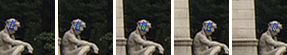
\includegraphics[width = .8\textwidth]{figs/patch_groups/patch_group_bus_045_085_012_s40_wx37_wt2_sx9_st4_r040_n200_coor.png}\\
	\vspace{.2cm}
	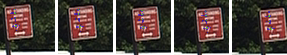
\includegraphics[width = .8\textwidth]{figs/patch_groups/patch_group_bus_255_056_010_s40_wx37_wt2_sx9_st4_r040_n200_coor.png}
%	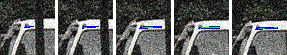
\includegraphics[width = .8\textwidth]{figs/patch_groups/patch_group_bus_110_090_010_s40_wx37_wt2_sx9_st4_r040_n200_coor.png}
	\caption{Examples of sets of 200 nearest neighbors spatio-temporal patches,
	for patches of size $9\times 9\times 4$.
	The images in each row show the five frames of a $37\times37\times5$ search region. 
	In red we show the positions of the 5 nearest neighbors, in green the next 40 and in blue the rest.
	Note that the points shown correspond to the top-left pixel of the first spatial
	slice of each patch.
	The reference patch is the red patch in the center of the search region. To highlight the
	position of the patches, the color of the images has been attenuated.}
	\label{fig:patch_groups_pos}
\end{figure*}

\begin{figure}[htpb!]
	\centering
%	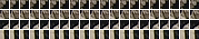
\includegraphics[width = .49\columnwidth]{figs/patch_groups/patch_group_bus_045_085_012_s40_wx37_wt2_sx9_st4_r040_n200_orig.png}
%	\hfill
%	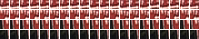
\includegraphics[width = .49\columnwidth]{figs/patch_groups/patch_group_bus_255_056_010_s40_wx37_wt2_sx9_st4_r040_n200_orig.png}\\
%	\vspace{.1cm}
	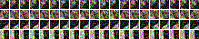
\includegraphics[width = .49\columnwidth]{figs/patch_groups/patch_group_bus_045_085_012_s40_wx37_wt2_sx9_st4_r040_n200_nisy.png}
	\hfill
	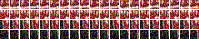
\includegraphics[width = .49\columnwidth]{figs/patch_groups/patch_group_bus_255_056_010_s40_wx37_wt2_sx9_st4_r040_n200_nisy.png}\\
	\vspace{.2cm}
	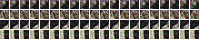
\includegraphics[width = .49\columnwidth]{figs/patch_groups/patch_group_bus_045_085_012_s40_wx37_wt2_sx9_st4_r040_n200_deno.png}
	\hfill
	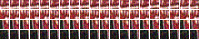
\includegraphics[width = .49\columnwidth]{figs/patch_groups/patch_group_bus_255_056_010_s40_wx37_wt2_sx9_st4_r040_n200_deno.png}\\
	\vspace{.2cm}
	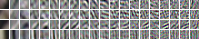
\includegraphics[width = .49\columnwidth]{figs/patch_groups/patch_group_bus_045_085_012_s40_wx37_wt2_sx9_st4_r040_n200_pcas.png}
	\hfill
	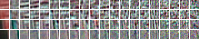
\includegraphics[width = .49\columnwidth]{figs/patch_groups/patch_group_bus_255_056_010_s40_wx37_wt2_sx9_st4_r040_n200_pcas.png}\\
	\vspace{.2cm}
	\caption{For each of the two sets of patches of Fig. \ref{fig:patch_groups_pos} we show
	the 20 nearest neighbors (top), the corresponding MAP estimates (middle) and the sample mean 
	and first 19 principal directions computed from the sample covariance matrix (bottom).
	For each image, each column corresponds to the 4 spatial slices of a $9\times9\times4$ patch.}
	\label{fig:patch_groups_patches}
\end{figure}

\section{Description of the algorithm}
\label{sec:algorithm}

Let us now describe the video denoising algorithm. As in
\cite{Dabov2007tip,Dabov2007v,Maggioni2012,Lebrun2013a} we perform two stages, described in 
Algorithms \ref{alg:nlbayes} and \ref{alg:nlbayes2}. In the first stage we
compute a \emph{basic} estimate, which we denote $\widetilde u^{(1)}$. 

In the second stage computes the final estimate $\widetilde u^{(2)}$ using the
basic estimate as an oracle. This entails two modifications with respect to the
first stage (highlighted in italics in Algorithm \ref{alg:nlbayes2}). Firstly, the
computation of the patch distances is performed using the patches of the basic
estimate instead of the noisy ones. And secondly, we assume that the patches of
the basic estimate are drawn from the \textit{a priori} Gaussian model and use
them to learn the mean and covariance matrix. Note that in the second stage,
when estimating the covariance matrix, we assume that the patches of the basic
estimate have no noise. Thus we set $\sigma = 0$ in Eq.
\eqref{eq:learn_parameters}.

\begin{algorithm}
	\caption{Video NL-Bayes - Step 1: basic estimate}
	\label{alg:nlbayes}
		\begin{algorithmic}[1]
		\REQUIRE Noisy video $v$, noise standard deviation
		$\sigma$
		\ENSURE Basic estimate of noiseless video $\widetilde u^{(1)}$
		\STATE Set $\mathcal P = \{\ma q \,:\, \ma q \text{ patch of }  v\}$ \COMMENT{patches to process}
		\WHILE{$\mathcal P \neq \emptyset$}
		\STATE Get a patch $\ma q$ from $\mathcal P$ \COMMENT{``center'' of Gaussian model}
			\STATE Retrieve  the $n$ nearest neighbors to $\ma
			q$ in a spatio-temporal volume around $\ma q$
			\STATE Compute $\widehat{\overline{\ma p}}\,\!^{(1)}$ and
			$\widehat C_{r}^{(1)}$ 
			\FORALL{$n$ neighbors $\ma q_i$ of $\ma q$}
				\STATE Obtain the MAP estimate $\widetilde{\ma p}_i^{(1)}$
				\STATE Aggregate estimated patch on $\widetilde u^{(1)}$
				\STATE Remove $\ma q_i$ from $\mathcal P$
			\ENDFOR
		\ENDWHILE
	\end{algorithmic}
\end{algorithm}

\begin{algorithm}
\caption{Video NL-Bayes - Step 2: final estimate}
	\label{alg:nlbayes2}
	\begin{spacing}{1.3}
		\begin{algorithmic}[1]
		\REQUIRE Noisy video $v$, noise standard
		deviation $\sigma$, \emph{basic estimate $\widetilde u^{(1)}$} 
		\ENSURE Final estimate of noiseless video $\widetilde u^{(2)}$
		\STATE Set $\mathcal P = \{\ma q \,:\, \ma q \text{ patch of }  v\}$ \COMMENT{patches to process}
		\WHILE{$\mathcal P \neq \emptyset$}
		\STATE Get a patch $\ma q$ from $\mathcal P$ \COMMENT{``center'' of Gaussian model}
			\STATE Retrieve the $n$ nearest neighbors to $\ma
			q$ in a spatio-temporal volume around $\ma q$.
			\emph{The distance is computed between the basic estimates
				$\widetilde{\ma p}^{(1)}$}
			\STATE Compute $\widehat{\overline{\ma p}}\,\!^{(2)}$ and $\widehat
					 C_{r}^{(2)}$ \emph{from the basic estimates
						 $\widetilde{\ma p}_i^{(1)}$, setting $\ma{\sigma = 0}$.}
			\FORALL{$n$ neighbors $\ma q_i$ of $\ma q$}
				\STATE Obtain the MAP estimate $\widetilde{\ma p}_i^{(2)}$
				\STATE Aggregate estimated patch on $\widetilde u^{(2)}$
				\STATE Remove $\ma q_i$ from $\mathcal P$
			\ENDFOR
		\ENDWHILE
	\end{algorithmic}
	\end{spacing}
\end{algorithm}

%\begin{algorithm}
%	\caption{Video NL-Bayes}
%	\label{alg:nlbayes}
%	\begin{algorithmic}
%		\REQUIRE Noisy video $v$, noise standard deviation $\sigma$ \\
%		\ENSURE Estimate of noiseless video $\widetilde u$
%		\FORALL{patches $\ma q$ in $v$}
%		\STATE Find the $n$ most similar patches to $\ma q$ in a search volume centered at $\ma q$
%		\STATE Compute $\widehat{\overline{\ma p}}\,\!^{(1)}$ and $\widehat C^{(1)}$ according to \eqref{eq:learn_parameters}
%		\STATE Obtain the first stage estimate $\widetilde{\ma p}^{(1)}$ by \eqref{eq:map}
%		\ENDFOR
%		\FORALL{pixel $(x,t)$ in $\Omega\times {1,\dots,T}$}
%		\STATE Obtain the basic estimate $\widetilde u^{(1)}(x,t)$ by averaging
%		the values of all patches $\widetilde{\ma p}^{(1)}$ containing $(x,t)$.
%		\ENDFOR
%		\FORALL{patches $\ma q$ in $v$}
%		\STATE Find the $n$ most similar patches to $\ma q$ in a
%		search volume centered at $\ma q$ by comparing the estimates $\widetilde{\ma
%		p}^{(1)}$. We denote them, and their corresponding basic estimates as 
%		$\ma q_i$ and $\widetilde{\ma p}_i^{(1)}$ respectively.
%		\STATE Compute $\widehat{\overline{\ma p}}\,\!^{(2)}$ and $\widehat C^{(2)}$ according to
%\[
%	\widehat{\overline{\ma p}}\,\!^{(2)} = \frac1{n}\sum_{i = 1}^{n}\widetilde{\ma p}_i^{(1)} \quad\text{and}\quad 
%	\widehat C^{(2)}= \frac1{nsum_{i = 1}^{n}\left(\widetilde{\ma p}_i^{(1)}\right)^T \widetilde{\ma p}_i^{(1)}.
%\]
%		\STATE Obtain the second stage estimate $\widetilde{\ma p}^{(2)}$ as in \eqref{eq:map}
%		\ENDFOR
%		\FORALL{pixel $(x,t)$ in $\Omega\times {1,\dots,T}$}
%		\STATE Obtain the final estimate $\widetilde u(x,t)$ by averaging
%		the values of all patches $\widetilde{\ma p}^{(2)}$ containing $(x,t)$.
%		\ENDFOR
%
%	\end{algorithmic}
%\end{algorithm}


%\begin{figure*}[thpb!]
%	\begin{center}
%		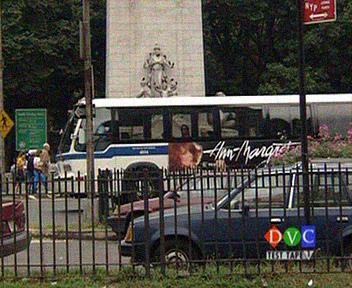
\includegraphics[trim=0.0cm 2.0cm 4.0cm 1.0cm, clip=true, width=0.25\textwidth]{figs/bus_nisy_s10_044.png}
%		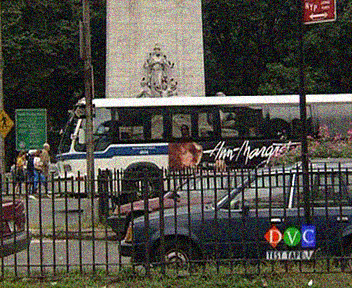
\includegraphics[trim=0.0cm 2.0cm 4.0cm 1.0cm, clip=true, width=0.25\textwidth]{figs/bus_nisy_s20_044.png}
%		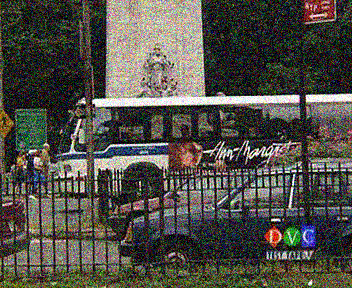
\includegraphics[trim=0.0cm 2.0cm 4.0cm 1.0cm, clip=true, width=0.25\textwidth]{figs/bus_nisy_s40_044.png}\\
%		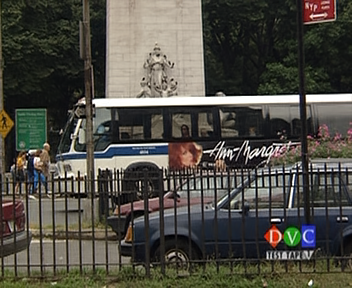
\includegraphics[trim=0.0cm 2.0cm 4.0cm 1.0cm, clip=true, width=0.25\textwidth]{figs/bus_vnlb_s10_tr2_044.png}
%		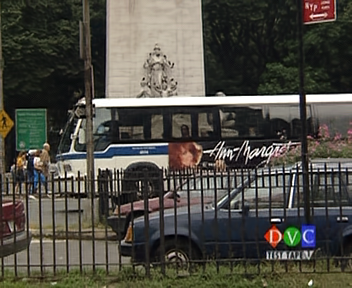
\includegraphics[trim=0.0cm 2.0cm 4.0cm 1.0cm, clip=true, width=0.25\textwidth]{figs/bus_vnlb_s20_tr2_044.png}
%		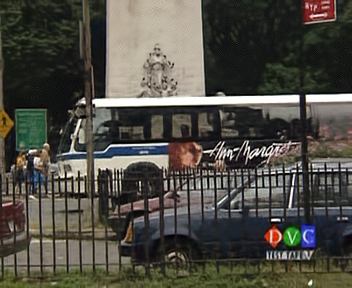
\includegraphics[trim=0.0cm 2.0cm 4.0cm 1.0cm, clip=true, width=0.25\textwidth]{figs/bus_vnlb_s40_tr2_044.png}\\
%		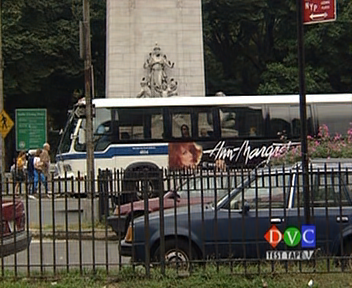
\includegraphics[trim=0.0cm 2.0cm 4.0cm 1.0cm, clip=true, width=0.25\textwidth]{figs/bus_s10_bm4d_044.png}
%		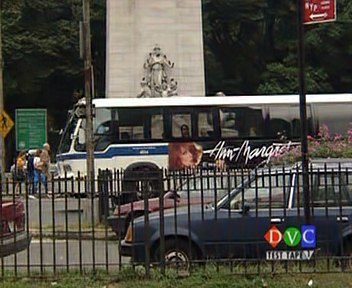
\includegraphics[trim=0.0cm 2.0cm 4.0cm 1.0cm, clip=true, width=0.25\textwidth]{figs/bus_s20_bm4d_044.png}
%		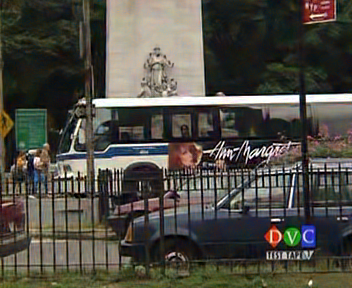
\includegraphics[trim=0.0cm 2.0cm 4.0cm 1.0cm, clip=true, width=0.25\textwidth]{figs/bus_s40_bm4d_044.png}\\
%		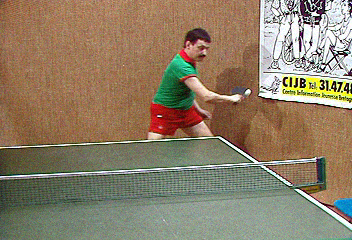
\includegraphics[trim=3.5cm 2.0cm 1.5cm 0.5cm, clip=true, width=0.25\textwidth]{figs/tennis_nisy_s10_140.png}
%		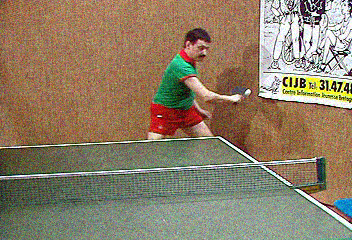
\includegraphics[trim=3.5cm 2.0cm 1.5cm 0.5cm, clip=true, width=0.25\textwidth]{figs/tennis_nisy_s20_140.png}
%		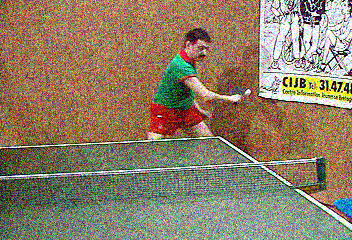
\includegraphics[trim=3.5cm 2.0cm 1.5cm 0.5cm, clip=true, width=0.25\textwidth]{figs/tennis_nisy_s40_140.png}\\
%		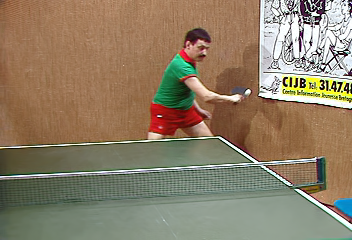
\includegraphics[trim=3.5cm 2.0cm 1.5cm 0.5cm, clip=true, width=0.25\textwidth]{figs/tennis_vnlb_s10_tr2_140.png}
%		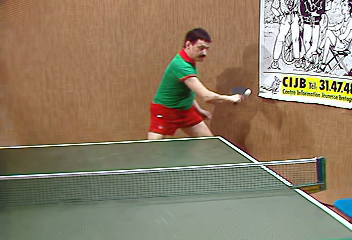
\includegraphics[trim=3.5cm 2.0cm 1.5cm 0.5cm, clip=true, width=0.25\textwidth]{figs/tennis_vnlb_s20_tr2_140.png}
%		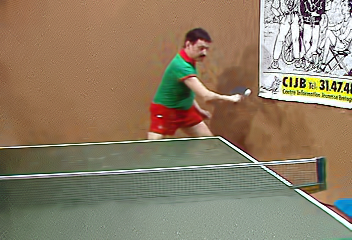
\includegraphics[trim=3.5cm 2.0cm 1.5cm 0.5cm, clip=true, width=0.25\textwidth]{figs/tennis_vnlb_s40_tr2_140.png}\\
%		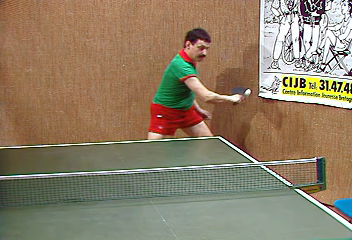
\includegraphics[trim=3.5cm 2.0cm 1.5cm 0.5cm, clip=true, width=0.25\textwidth]{figs/tennis_s10_bm4d_140.png}
%		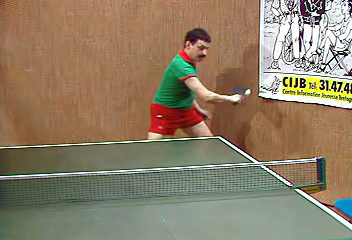
\includegraphics[trim=3.5cm 2.0cm 1.5cm 0.5cm, clip=true, width=0.25\textwidth]{figs/tennis_s20_bm4d_140.png}
%		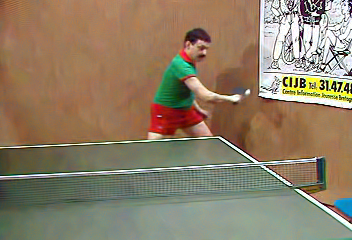
\includegraphics[trim=3.5cm 2.0cm 1.5cm 0.5cm, clip=true, width=0.25\textwidth]{figs/tennis_s40_bm4d_140.png}
%	\end{center}
%	\caption{Comparison of results obtained with VNLB ($w_t =5$) and V-BM4D-np.
%	The first three rows, correspond to a frame of the bus sequence. From top to
%	bottom: noisy input data. The last three rows correspond to the tennis sequence.
%	Each column shows results obtained for $\sigma = 10$, $20$ and $40$.}
%	\label{fig:results}
%\end{figure*}

\subsection{Implementation details}
\label{sse:implementation}

\paragraph{Handling of color} %Color videos are handled as in \cite{Lebrun2013a}.
%
In the first stage, we express the video in a luminance-chrominance color space,
specifically we apply the opponent color transform (see \cite{Dabov2007tip,Lebrun2013a}).
Patch distances are computed using the luminance only. Using the 
$n$ most similar patches, a group is built for each channel. These
groups are filtered independently (a Gaussian model is learnt for each of them).
%
In the second stage, the patch distance is computed using the RGB patches, and
a joint \textit{a priori} Gaussian model is built for each set
of similar RGB patches. Note that in first stage, we learn three Gaussian models
of dimensionality $s_x^2s_t$, whereas in the second stage we learn a single 
Gaussian model of tripled dimensionality.

% \paragraph{Variance correction factor} In practice, when computing the MAP
% estimate by eq. \eqref{eq:map}, we introduce a parameter $\beta$ (with $\beta \approx 1$) multiplying
% $\sigma^2I$ to be able to control the amount of filtering.

\paragraph{Patch distance threshold} When building the group of similar
patches during the second stage, more than $n$ patches are allowed
if their distances with respect to the reference patch are smaller than a
threshold $\tau$.  As in \cite{Lebrun2013ipol}, we set $\tau = 4$ (the distance between
patches is normalized by the number of elements in the patch and the number of
channels and the values of each channel are in the range  $[0,255]$).


\subsection{Computational complexity and speed-ups}
\label{sse:complexity}

Let us consider the complexity of constructing and filtering a group of
$n$ similar patches.
Processing each group of similar patches is of asymptotic order $\mathcal
O(w_x^2 w_t s_x^2 s_t + ns_x^4s_t^2 + s_x^4s_t^2r)$.
The first term comes from the exhaustive search of the $n$ nearest patches in
the search window.  The remaining terms correspond respectively to the
computation of the covariance matrix and its truncated spectral decomposition.

The most expensive operations are the computation of the covariance matrix and
of its principal directions.
There are methods for computing the $r$ principal directions
of a set of points that do not require computing the covariance matrix
\cite{Halko2011}. Instead these methods efficiently approximate a truncated SVD
of the data matrix, and would 
allow to improve the computational complexity to $\mathcal O(w_x^2 w_t s_x^2
s_t + s_x^2s_trn)$.


The computation can be substantially accelerated by reducing the 
number of groups of patches that are jointly processed.
Each group of patches is associated to the reference patch from which 
the nearest neighbors are computed.
We apply two tricks
considered in \cite{Dabov2007tip,Lebrun2013ipol} in order to reduce the number of reference patches. 
The first one consists on visiting only 
those patches on a coarser spatial grid with vertical and horizontal separation
of $s_x/2$. This reduces the number of reference patches by a factor of
$s_x^2/4$. The second trick consists on the following.  After
filtering the patches in a group, these patches are not considered again
as reference patches. 
Note that we ensure that each reference patch is filtered at least once. 
Due to the spacing of the coarse grid, this guarantees that each pixel is
overlapped by four reference patches on the same frame, so it will receive at
least four contributions in the aggregation. The actual number of aggregated
estimates for each pixel is much higher, considering the reference and
non-reference patches (which can also be filtered) in the neighboring frames.

Due to these speed-ups, the actual number of groups of similar patches processed
depends on $n$, and varies between a $1\%$ ($n \approx 400$)  and a $10\%$ ($n
\approx 50$) of the total number of pixels in the sequence. 
\pcomment{Check this numbers!}


\section{Discussion}
\label{sec:discussion}

\subsection{Spatio-temporal patches}
\label{sse:spatio-temporal-patches}
Patch-based methods filter similar patches to remove noise. When the noise is
Gaussian, the patch similarity is determined based on the (squared) Euclidean distance 
between patches. Due to the noise, the Euclidean distance follows a non-central
$\chi^2$ distribution, with variance
\[\textnormal{Var}\left\{\frac1{m}\|\ma q_1 - \ma q_2\|^2\right\} = \frac{8\sigma^2}{m}\left(\sigma^2 + \frac1{m}\|\ma p_1 - \ma p_2\|^2\right),\]
where $\ma q_1, \ma q_2$ are the noisy versions of the patches $\ma p_1, \ma p_2$, 
and $m$ denotes the number of pixels in the patch. The noise in the patch comparison
can be reduced by considering larger patches.
However, increasing the size of the patch also increases the distances between
patches and reduces the likelihood of finding similar patches.
%
The additional temporal dimension in a spatio-temporal patch allows to increase
the number of pixels in the patch, without increasing its spatial size.
Due to the high redundancy of the video in the temporal dimension, increasing the 
temporal size of the patch causes a much lower increase in the patch distances.
%The high redundancy of the video in the temporal dimension, allows to have 
%larger patches without affecting much the number of nearest neighbors of the patch.
%

Let us assume that 
the brightness of the original video is constant along motion trajectories, so
that $u(x,t + \tau) = u(\varphi(x,t + \tau; -\tau),t)$, where
$\varphi(x,t+\tau;\, \cdot\, )$ denotes the motion trajectory passing through
$(x,t + \tau)$.
Furthermore, let us assume that the motion in the video is approximately
translational.
When the motion is known or can be estimated, then it is natural to consider
motion compensated spatio-temporal patches. 
With the assumptions we are considering, all spatial slices of a $s_x\times s_x\times s_t$ motion-compensated patch
coincide, so the distance between two spatio-temporal patches is proportional to
the distance of a 2D spatial patch of size $s_x\times s_x$.
%
As a consequence, by increasing $s_t$, one can reduce the 
noise in the patch distance and have the same pattern of self-similarity as a 
2D patch.

However, motion estimation is challenging, and even more so in the presence of noise.
%Most motion estimation techniques integrate spatial information either 
%by matching 2D patches (or blocks, as they are commonly referred to in the
%motion estimation literature) or by some spatial regularization term in an energy.
An option that does not require motion is to use rectangular spatio-temporal patches.
The distance between these can be also expressed as a distance between spatial patches,
but their equivalent spatial support is larger than $s_x\times s_x$.

%To see this, let us observe that the squared Euclidean distance can be expressed as
%the convolution with a separable kernel.
To see this, let us assume that the motion in the video is a constant translation $v$. 
The squared Euclidean distance can be expressed as
%\begin{multline*}
%	d(\ma p_{xt}, \ma p_{ys})\\ %= [g_x\ast_x g_t \ast_t \left(u(x + \,\cdot\,,t + \,\cdot\,) -  u(y + \,\cdot\,,s + \,\cdot\,)\right)^2](0,0)\\
%		 = \iint g_x(\rho)g_t(\tau) \left(u(x + \rho,t + \tau) -  u(y + \rho,s + \tau)\right)^2d\tau d\rho
%\end{multline*}
\[
	d(\ma p_{xt}, \ma p_{ys}) = \iint g_x(\rho)g_t(\tau) f(\rho,\tau)d\tau d\rho
\]
where
%$\ast_x, \ast_t$ denote the spatial and temporal convolution operators and 
$f(\rho,\tau) = \left(u(x + \rho,t + \tau) -  u(y + \rho,s + \tau)\right)^2$,
and 
$g_xg_t$ is a separable spatio-temporal kernel which defines the
shape of the spatio-temporal patch. For example, for a rectangular patch, $g_x$
and $g_t$ are both box filters of sizes $s_x\times s_x$ and $s_t$ respectively.
Because of the brightness constancy assumption, we have that $f(\rho,\tau) = f(\rho + v\tau, 0)$.
%\pcomment{Note: this only holds if the motion at $t$ is equal than the one at $s$.}
Using this fact, after some manipulations we can rewrite the distance as a distance between 2D patches:
\[
	d(\ma p_{xt}, \ma p_{ys}) = \int f(\rho,0)h(\rho) d\rho
\]
where \[h(\rho) = \int g_x(\rho - v\tau)g_t(\tau)  d\tau\] is the 
equivalent spatial kernel. Note that this kernel is the result of integrating
several shifted versions of the spatial patch kernel $g_x$ along a motion trajectory.
%
Thus, when the brightness constancy assumption holds under a constant
translational motion $v$, the rectangular spatio-temporal patch is equivalent
to a spatial patch whose support depends on $v$. When $v = 0$, then it reduces 
to the $s_x\times s_x$ patch, and grows in the direction of the motion at $v$
increases.
%
In these settings, rectangular spatio-temporal patches can be expected to perform as well
as motion-compensated patches. 

For more complex types of motion, using rectangular spatio-temporal patches will result in
a larger variability in the set of nearest neighbors of a given patch, due to the fact that
both the spatial texture and the motion pattern may vary. At least in principle, better 
results should be obtained using motion compensation. However, in practice, the bad quality of
the estimated motion undermines the final result.


%\begin{align*}
%	d(\ma p_{xt}, \ma p_{ys}) %= [g_x\ast_x g_t \ast_t \left(u(x + \,\cdot\,,t + \,\cdot\,) -  u(y + \,\cdot\,,s + \,\cdot\,)\right)^2](0,0)\\
%		 &= \iint g_x(\rho)g_t(\tau) f(\rho,\tau)d\tau d\rho\\
%		 &= \iint g_x(\rho)g_t(\tau) f(\rho + v(\tau),0) d\tau d\rho\\
%		 &= \iint g_x(\rho - v(\tau))g_t(\tau) f(\rho,0) d\tau d\rho\\
%		 &= \int f(\rho,0)\int g_x(\rho - v(\tau))g_t(\tau)  d\tau d\rho\\
%		 &= \int f(\rho,0)h(\rho) d\rho\\
%\end{align*}



%after some manipulations the distance 
%can be written as the convolution with a spatial kernel:
%\begin{equation*}
%	d(\ma p_{xt}, \ma p_{ys}) = [h \ast_x \left(u(x + \,\cdot\,,t) -  u(y + \,\cdot\,,s)\right)^2](0),
%\end{equation*}
%where 
%\[
%	h(\xi) = [g_t \ast g_x(v\,\cdot\,)](\xi/v) 
%		= \int g_t(\eta)g_x(\xi - v\eta)d\eta.
%\]



% \pcomment{
% \begin{itemize}
% %	\item Justify why 3D patches: Greater distance noise reduction with roughly the same 
% %		degree of self-similarity. One way to see this is that the 3D patches can be 
% %		seen, for a video in which the brightness constancy assumption holds, as a 2D patch
% %		by back-projecting all the slices to the first frame.
% 	\item Relation with respect other iterative methods found in the literature
% 		(SOS, twicing, diffusion, BM3D, I-SA-BM4D).
% %	\item Variation of the results tables for different sequences.
% \end{itemize}}

\subsection{Estimation of the covariance matrix}
\label{sse:covariance-estimation}


Learning the parameters of the \emph{a priori} distribution for each group of
noisy patches amounts to estimating a covariance matrix in a high dimensional space 
and with a limited number of samples. 
%The latter is controlled by the $n$ parameter, which
%should not be too high in order for the Gaussian prior to be valid.
%
The empirical covariance matrix $\widehat C$ converges to the true covariance matrix
$C$ as the number of samples from the underlying Gaussian distribution grows to infinity.
But in our case, the number of samples we can ``draw'' from the Gaussian is limited:
%The Gaussian is only an approximate density model for the set of
%$n$ nearest neighbors of a target patch.
As we increase the number $n$ of neighbors of a patch, we include patches
that are not as similar to the reference patch and the Gaussian model becomes less valid. 

Thus there is a trade-off between accuracy of Gaussian model and precision of the
covariance matrix. We will find a compromise to this trade-off empirically  in
\S \ref{sec:parameters}.


The problem of estimating the covariance matrix has received a lot of attention in the
past ten years.
According to \cite{Vershynin2012}, the number of samples needed to achieve a given approximation
error between the empirical and the true covariances grows linearly with the
dimensionality of the space spanned by the data. 
%\pcomment{Comment: Actually, I found results relating the number of samples with
%the dimensionality of the ambient space. 
%However, if the data lies in a $p$-dimensional subspace, one could 
%compute a basis of this subspace from $n > p$ samples, and work in the low-dim
%coordinates to estimate a covariance matrix there. In that way, one could build
%a covariance matrix in the ambient space.}
%\pcomment{Comment: This reference may not be as relevant, in the light of the 
%results known for Gaussian covariance matrices. It would be interesting to see what 
%\cite{bunea2015} says regarding covariance matrices with low-effective rank.}

The rank also plays a role in the estimation of the covariance matrix.
As explained in \S \ref{sse:complexity}, alleviating the computational cost is
one of the reasons for using a low rank approximation of the empirical
covariance matrix. But there are also good reasons regarding the denoising
performance. In situations in which the number of samples 
is comparable to their dimension, the spectral decomposition of the empirical
covariance matrix $\widehat C$ can have considerable errors with respect to
that of the population covariance matrix $C$. 
%
The case of Gaussian models with covariance matrices of the form $C = A + \sigma^2I$,
where $A$ does not have full rank, has been studied in the statistics and physics
literature. The authors in \cite{johnstone2009,paul2007,nadler2008} study the
limit when the number of samples $n$ and the dimension $p$ grow to infinity at
same rate, such that $p/n\to\gamma < \infty$.  These works show that, for a
non-zero ratio $\gamma$, the empirical eigenvectors 
and eigenvalues are inconsistent estimators of the population ones.
Furthermore, the smaller eigenvalues and their eigenvectors will have a higher
error and eventually, if the signal-to-noise ratio drops bellow $\sqrt{\gamma}$, 
the eigenvector is confused with the noise and the resulting estimate will be,
in expectation, orthogonal to the actual value.
Finite sample bounds for the eigenvalues and eigenvectors have been also studied 
by \cite{nadler2008}, in the case in which $A$ has rank 1.
\pcomment{What can we say about this bounds.}

The errors between the sample eigenvectors and their population
counterparts manifest themselves as noise, which then affects the MAP estimate.
%
These asymptotic results suggest to discard the eigenvectors associated with 
lower eigenvalues. How many should be discarded in practice when $n$ and $p$ are finite, 
can only be fixed empirically, as we do in \$ \ref{sec:parameters}.

\pcomment{Results of Bunea are still missing!}
\pcomment{More detailed explanation of the results?}

\section{Parameter selection}
\label{sec:parameters}

For each stage of the algorithm we need to specify 6 parameters: the spatial
and temporal components of the patch size, $s_x$ and $s_t$, the spatial and
temporal components of the search region, $w_x$ and $w_t$, the number of similar
patches $n$ and the rank of the \textit{a priori} covariance matrix $r$.
When needed, we will add a subscript indicating the stage, \eg
$n_{1}$ and $n_{2}$.
We will consider different parameter settings for color and grayscale videos.



\begin{figure*}[htpb!]
	\begin{center}
		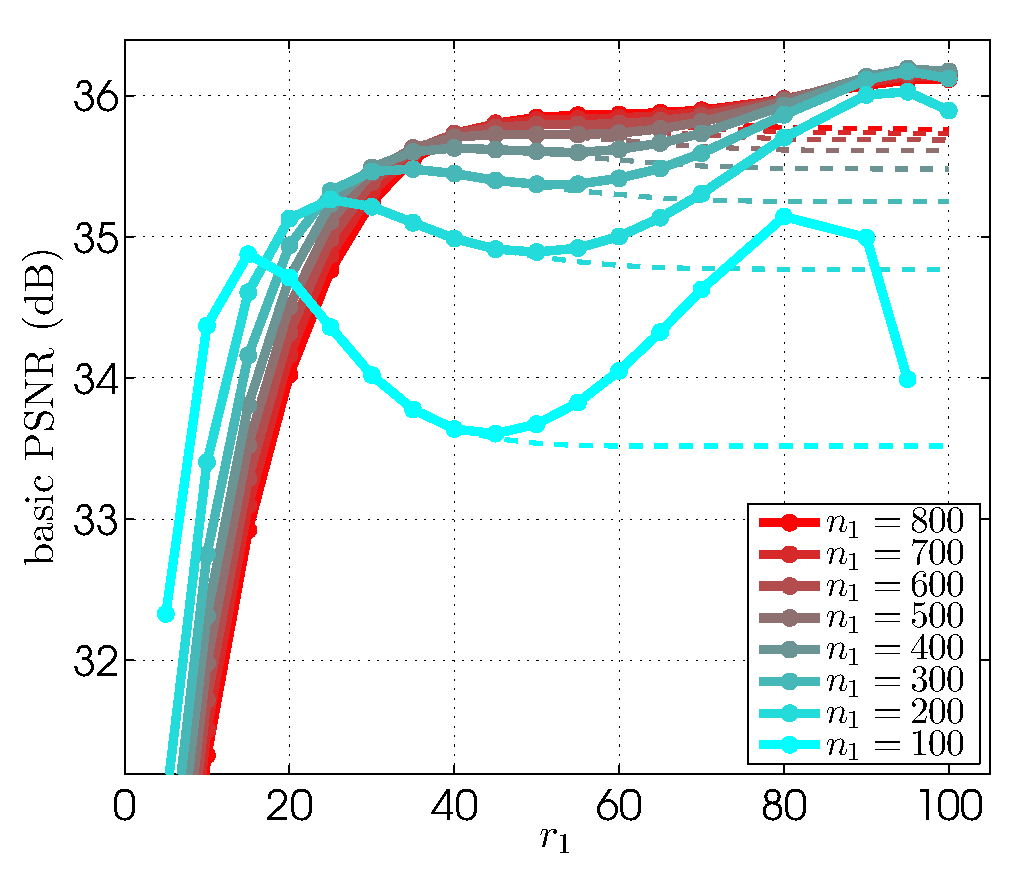
\includegraphics[width=.25\textwidth]{figs/params_tables/bpsnr_r1-np1-curves_s10_average_derf_neg-vs-pos-weights.eps}%
		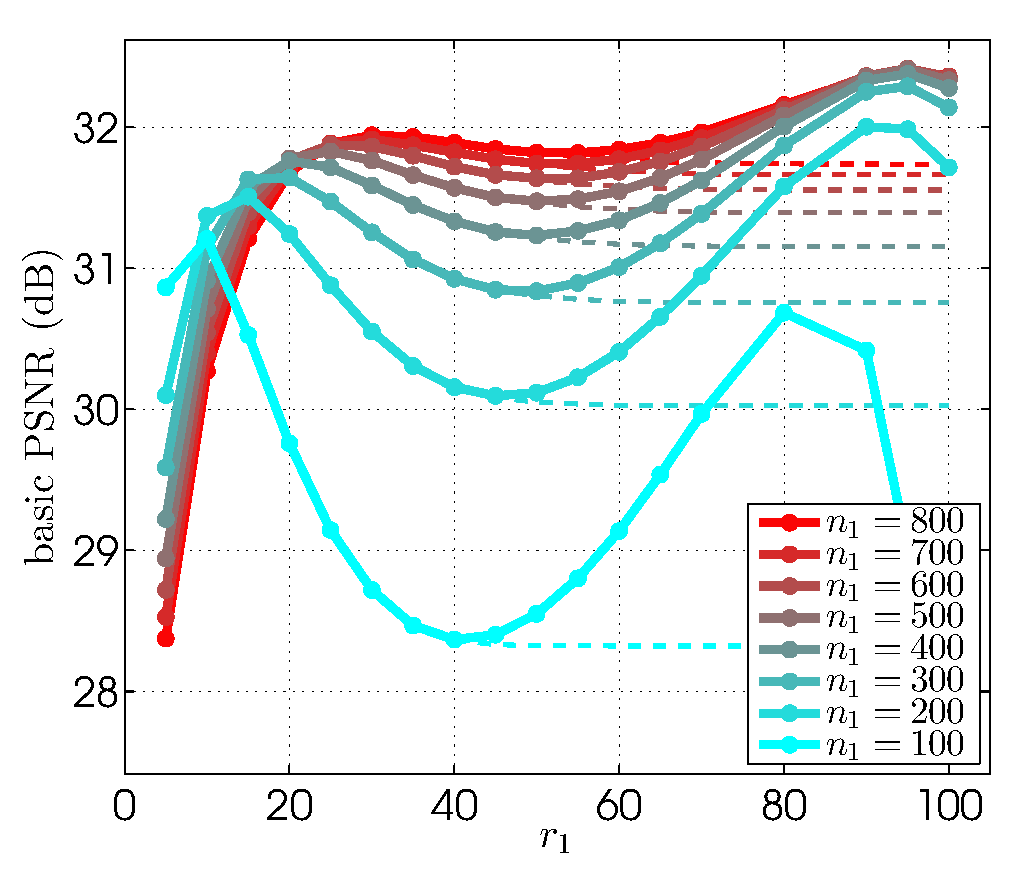
\includegraphics[width=.25\textwidth]{figs/params_tables/bpsnr_r1-np1-curves_s20_average_derf_neg-vs-pos-weights.eps}%
		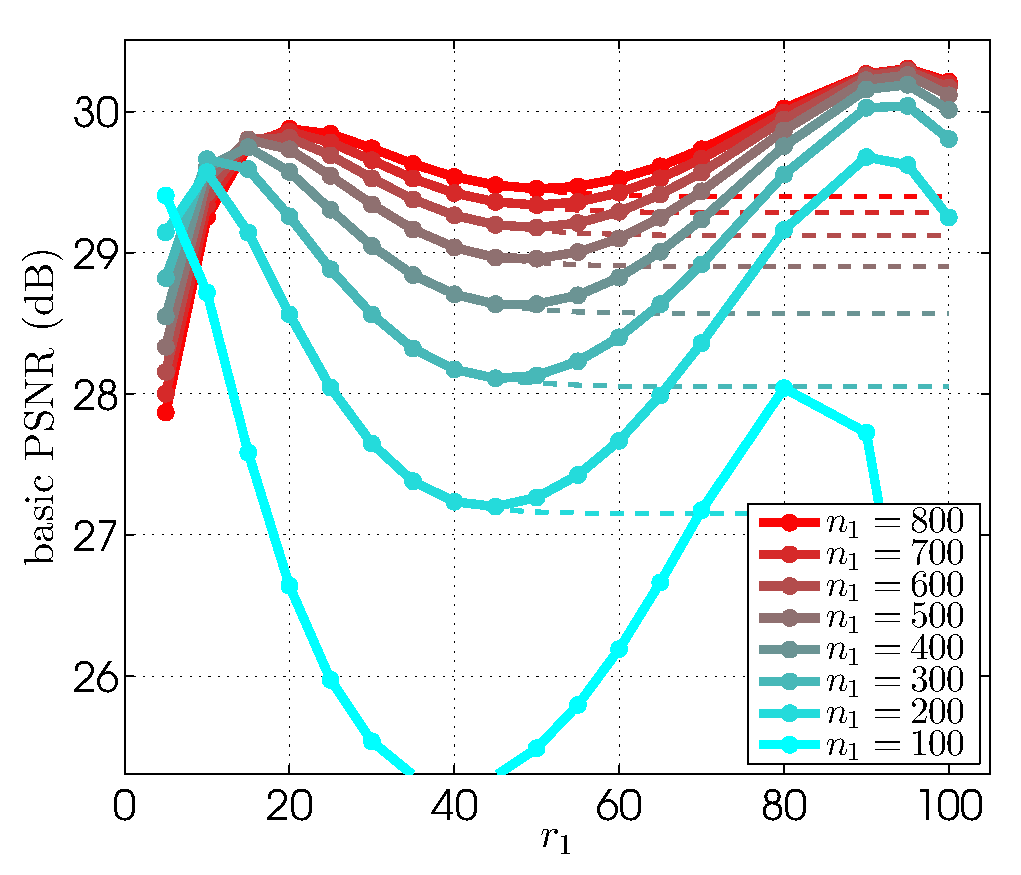
\includegraphics[width=.25\textwidth]{figs/params_tables/bpsnr_r1-np1-curves_s30_average_derf_neg-vs-pos-weights.eps}%
		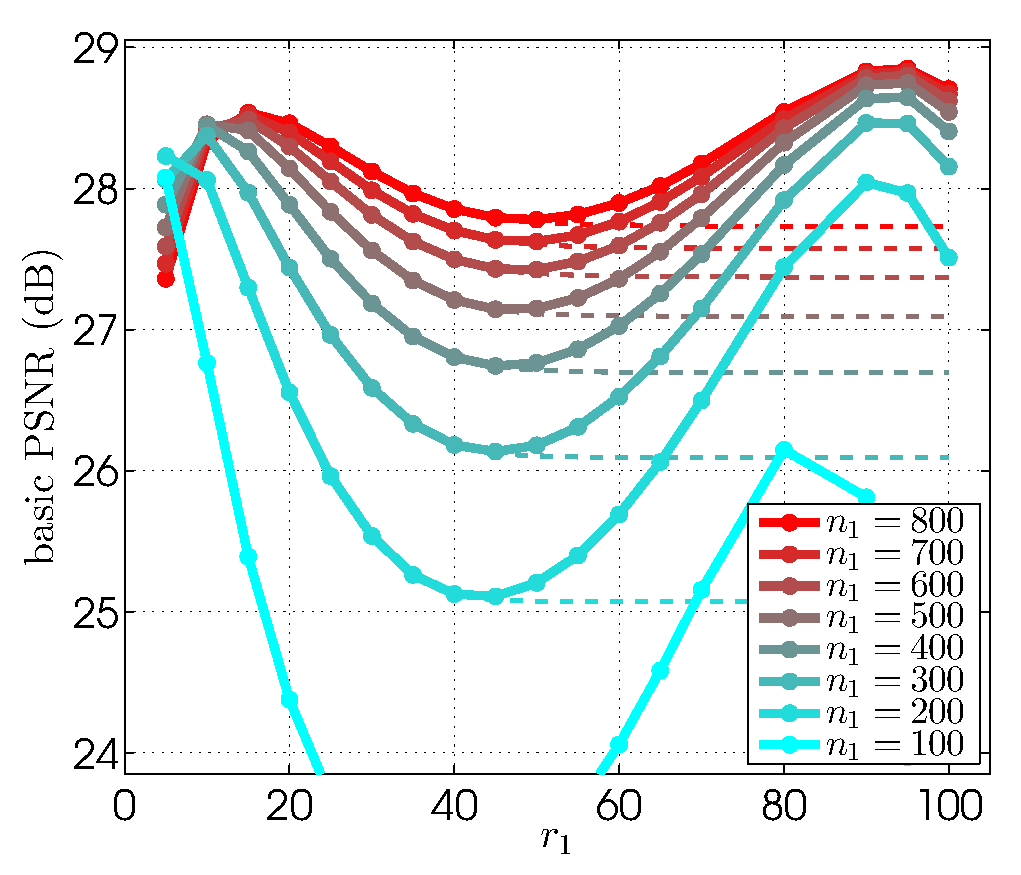
\includegraphics[width=.25\textwidth]{figs/params_tables/bpsnr_r1-np1-curves_s40_average_derf_neg-vs-pos-weights.eps}\\

		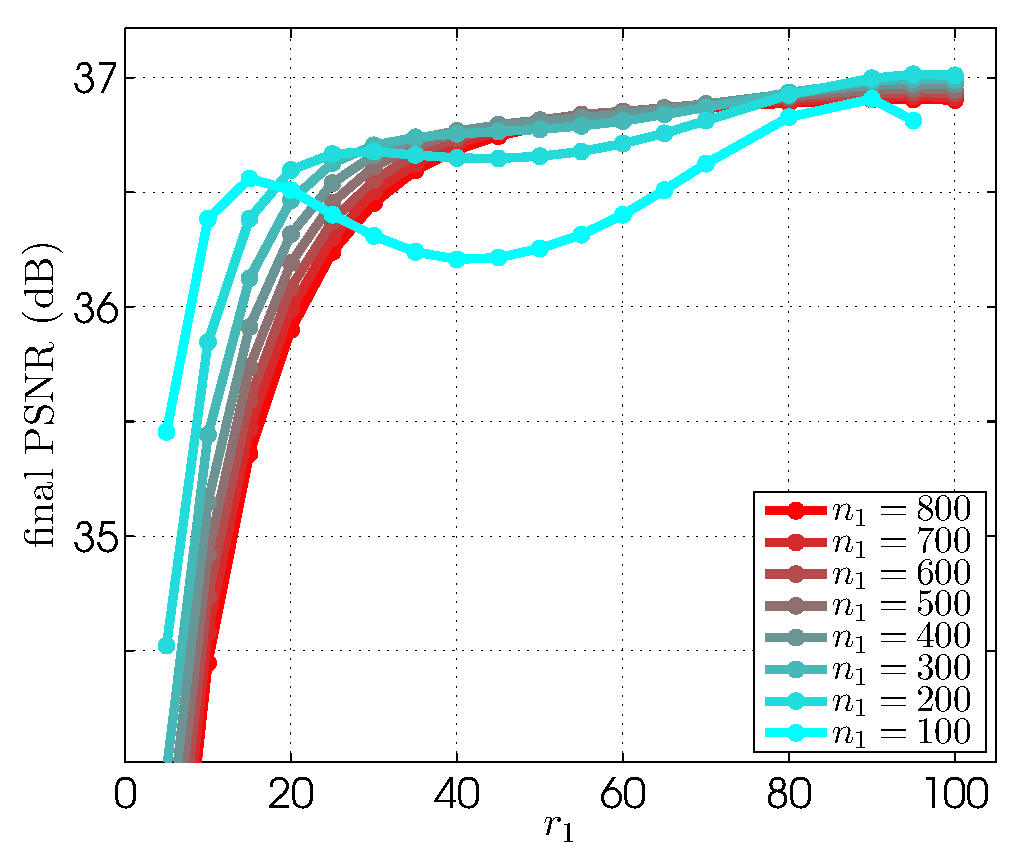
\includegraphics[width=.25\textwidth]{figs/params_tables/fpsnr_r1-np1-curves_s10_average_derf_neg-weights.eps}%
		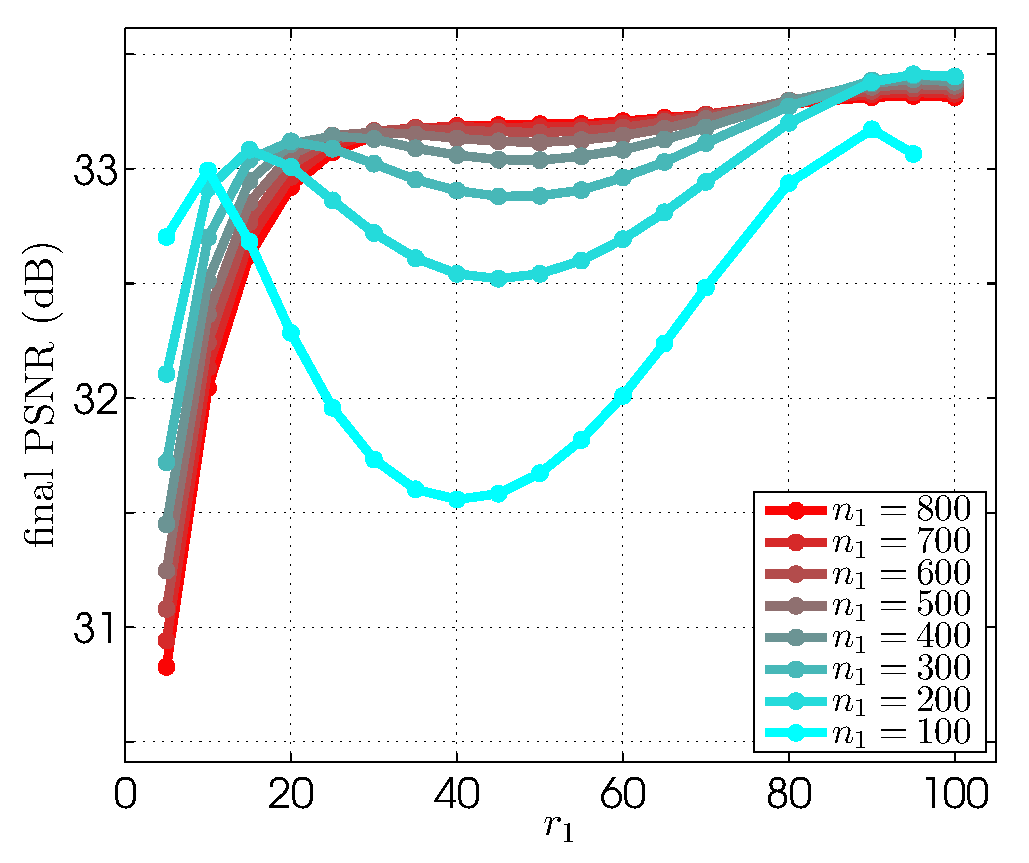
\includegraphics[width=.25\textwidth]{figs/params_tables/fpsnr_r1-np1-curves_s20_average_derf_neg-weights.eps}%
		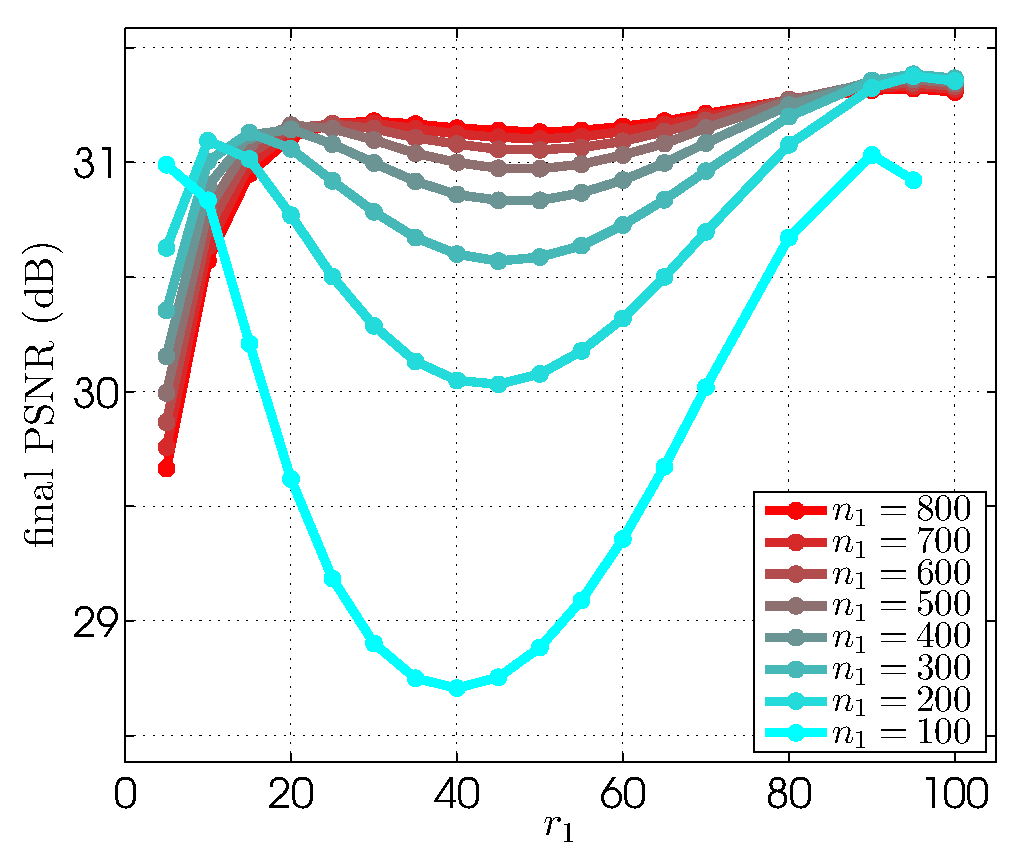
\includegraphics[width=.25\textwidth]{figs/params_tables/fpsnr_r1-np1-curves_s30_average_derf_neg-weights.eps}%
		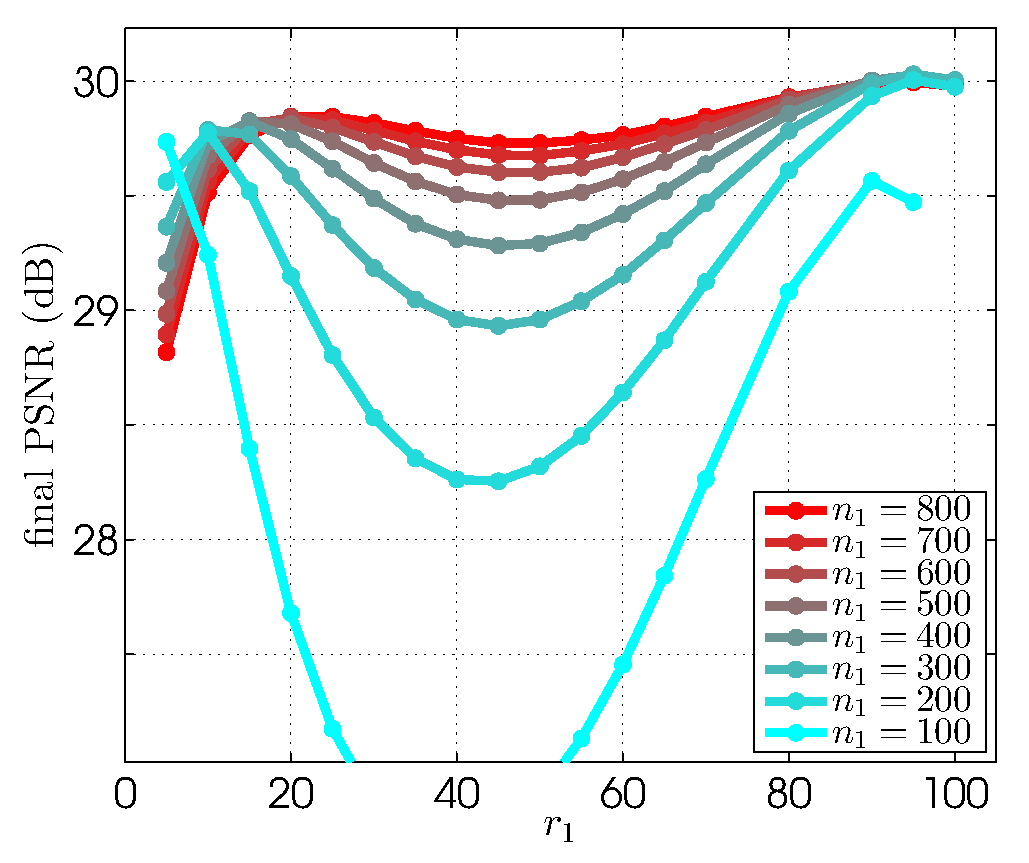
\includegraphics[width=.25\textwidth]{figs/params_tables/fpsnr_r1-np1-curves_s40_average_derf_neg-weights.eps}\\
	\end{center}
	\caption{PSNR averaged over four color sequences, when varying the
		first stage parameters $r_1$ and $n_1$. Top row, PSNR of the basic
		estimate; bottom row: final estimate. From left to right, results for
		$\sigma = 10, 20, 30, 40$.} 
	\label{fig:rank1-nsim1-psnr-color}

	\begin{center}
		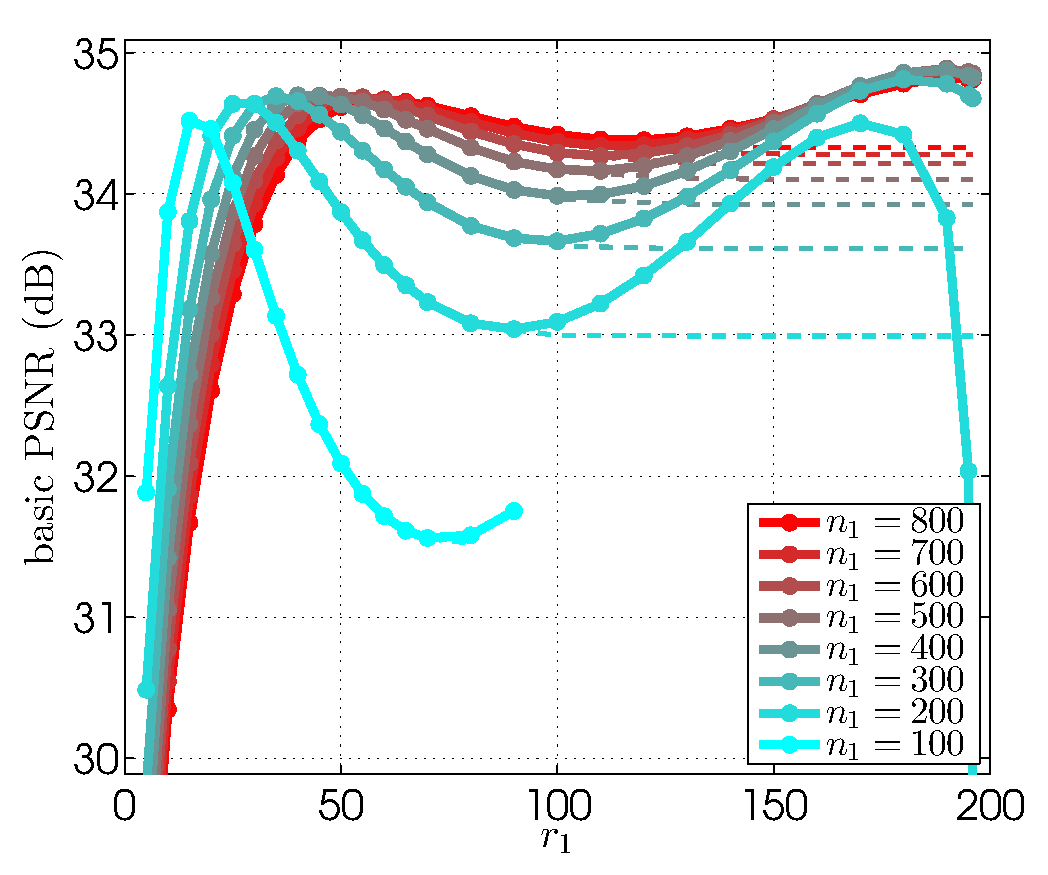
\includegraphics[width=.25\textwidth]{figs/params_tables/bpsnr_r1-np1-curves_s10_average_mono_neg-vs-pos-weights.eps}%
		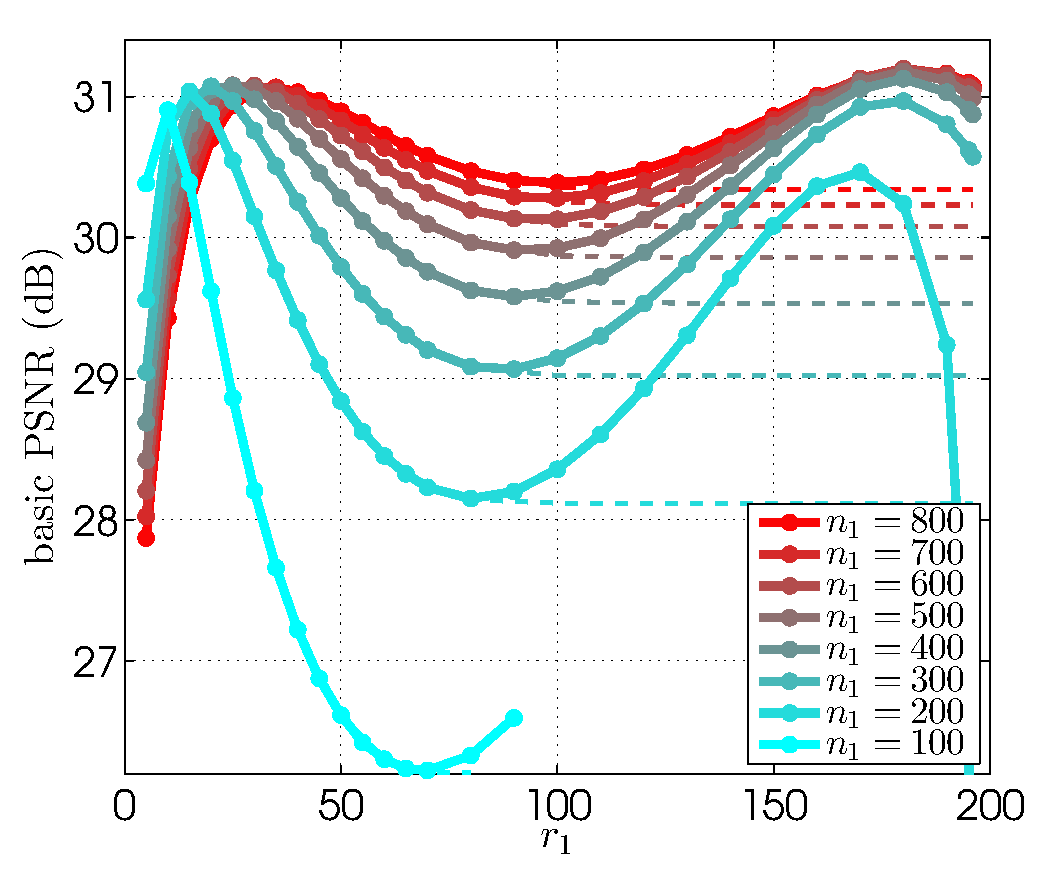
\includegraphics[width=.25\textwidth]{figs/params_tables/bpsnr_r1-np1-curves_s20_average_mono_neg-vs-pos-weights.eps}%
		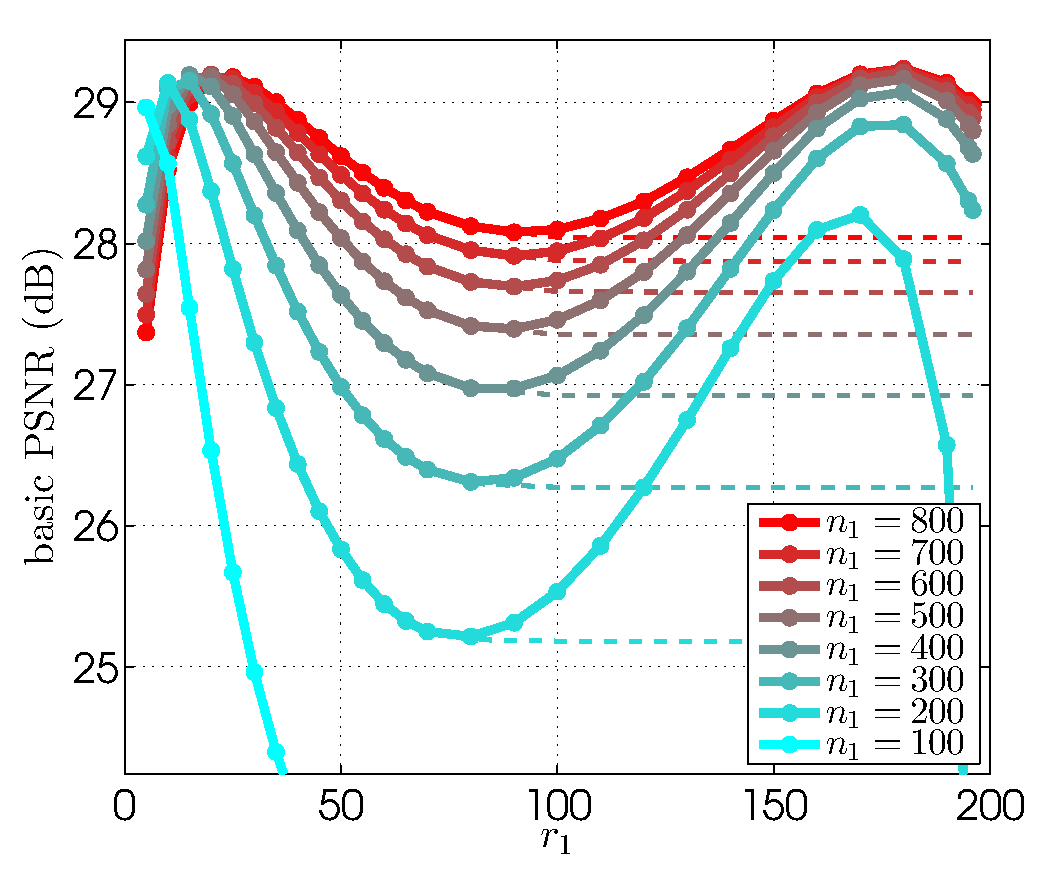
\includegraphics[width=.25\textwidth]{figs/params_tables/bpsnr_r1-np1-curves_s30_average_mono_neg-vs-pos-weights.eps}%
		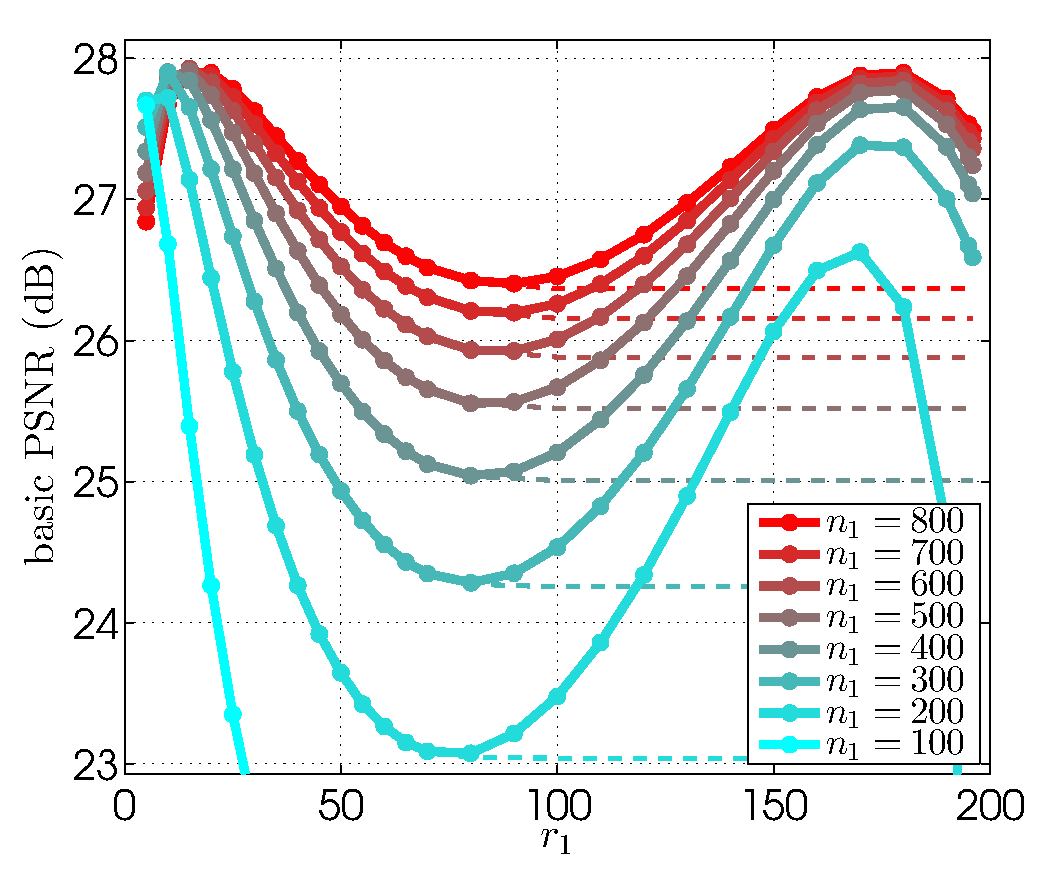
\includegraphics[width=.25\textwidth]{figs/params_tables/bpsnr_r1-np1-curves_s40_average_mono_neg-vs-pos-weights.eps}\\

		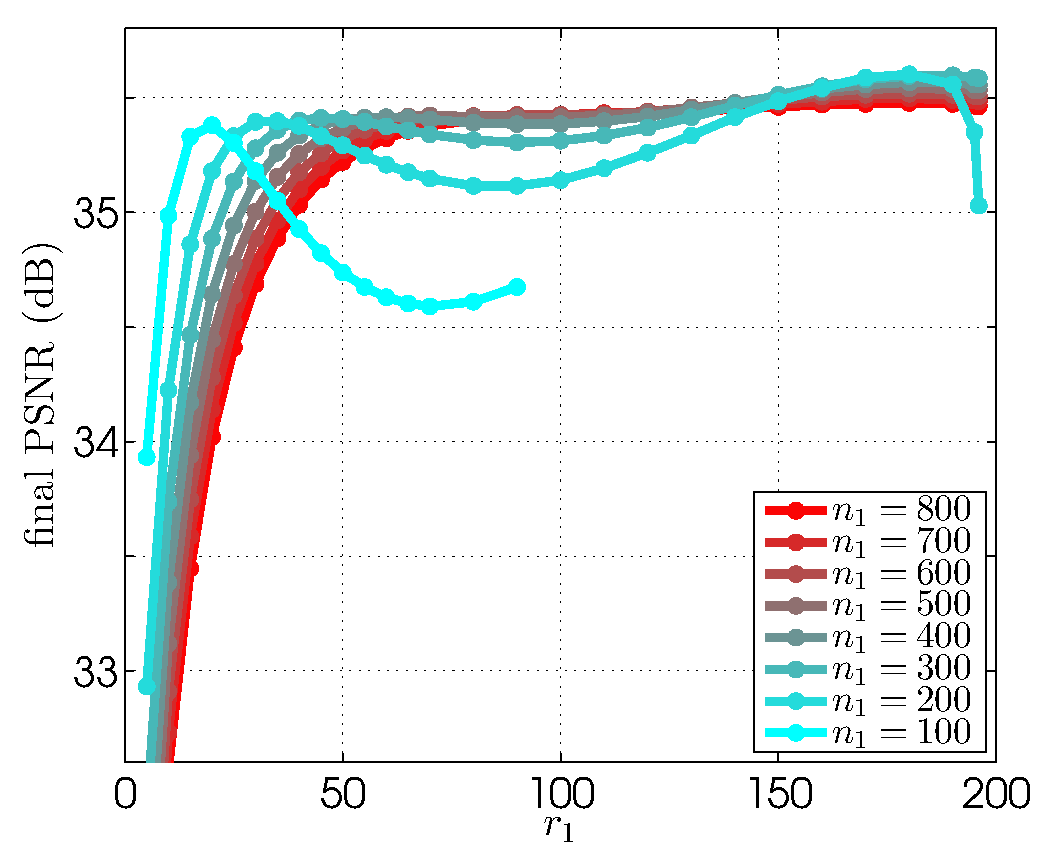
\includegraphics[width=.25\textwidth]{figs/params_tables/fpsnr_r1-np1-curves_s10_average_mono_neg-weights.eps}%
		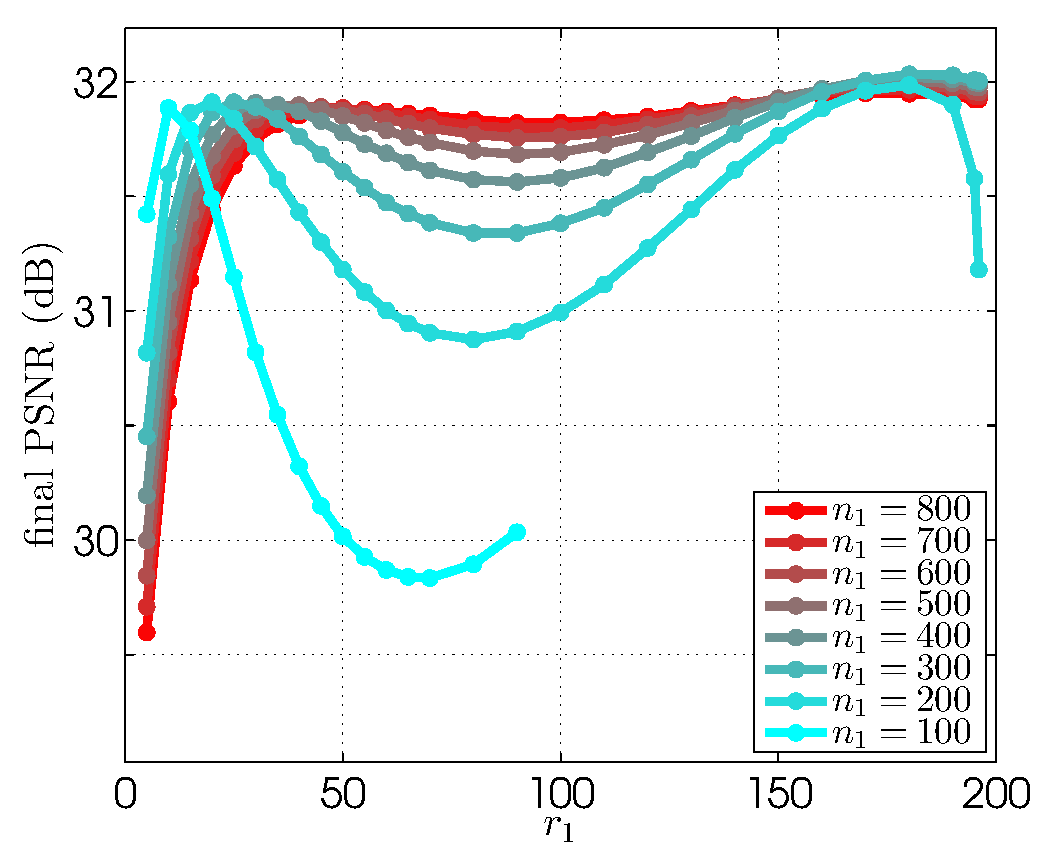
\includegraphics[width=.25\textwidth]{figs/params_tables/fpsnr_r1-np1-curves_s20_average_mono_neg-weights.eps}%
		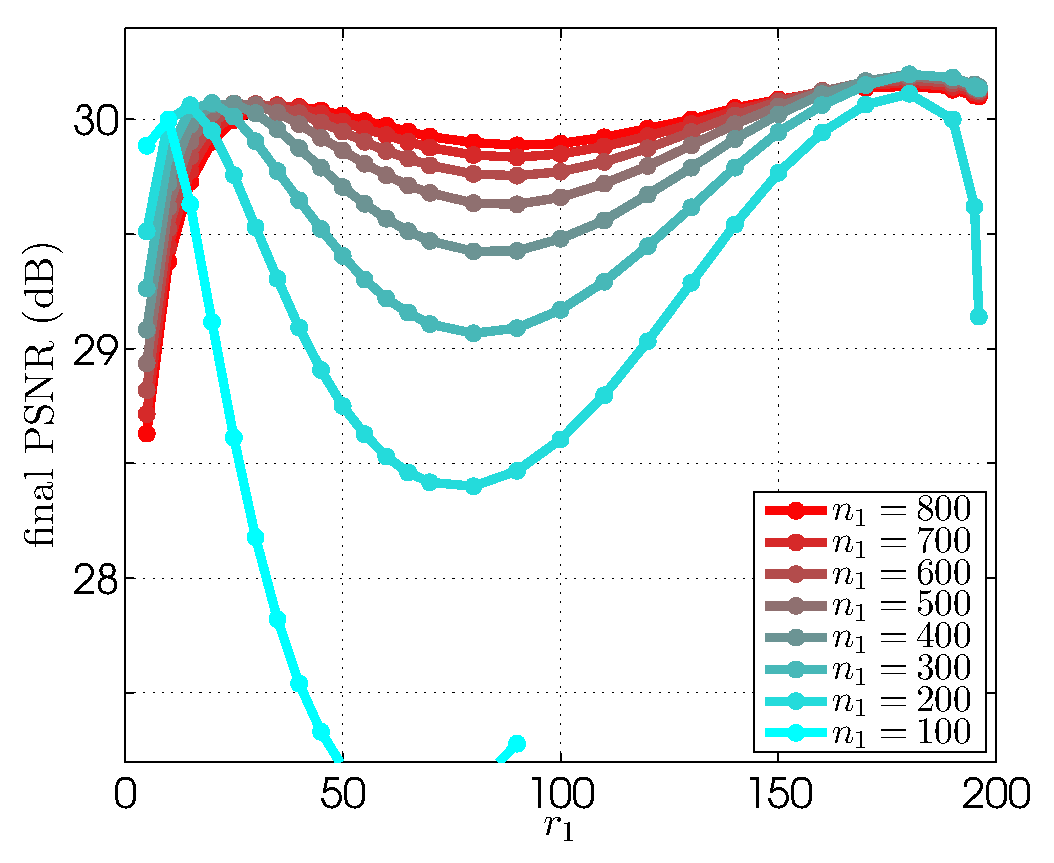
\includegraphics[width=.25\textwidth]{figs/params_tables/fpsnr_r1-np1-curves_s30_average_mono_neg-weights.eps}%
		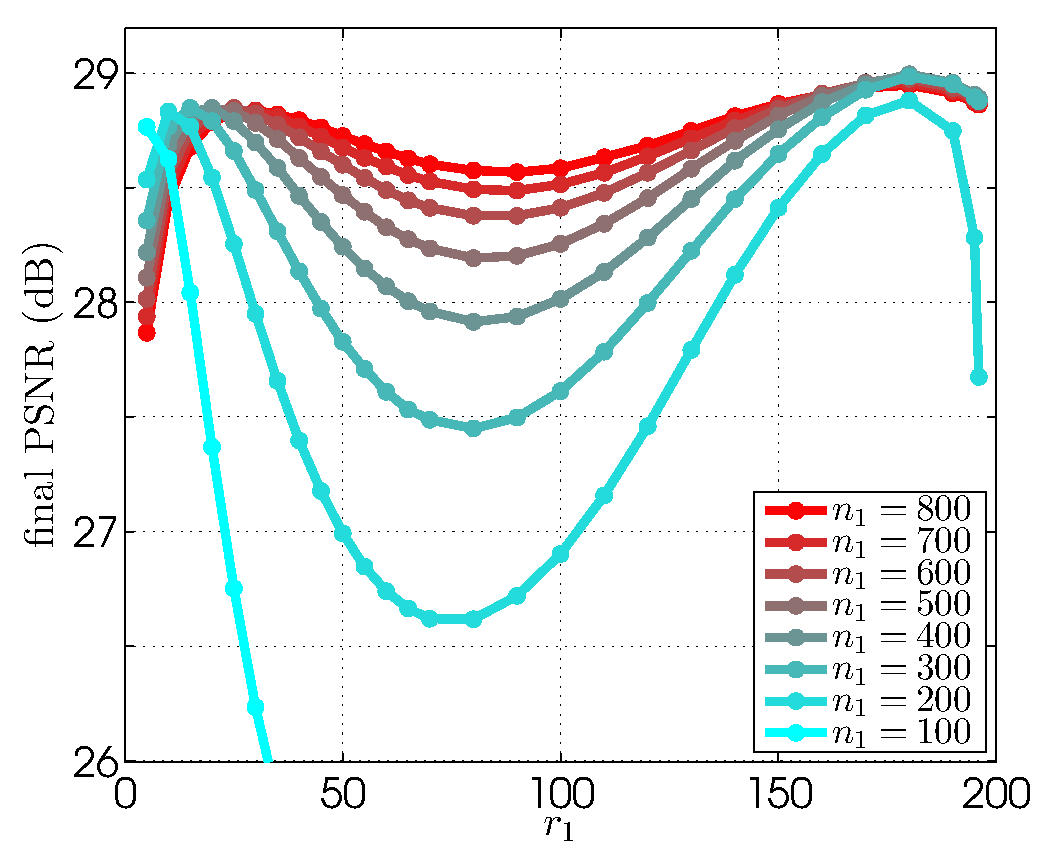
\includegraphics[width=.25\textwidth]{figs/params_tables/fpsnr_r1-np1-curves_s40_average_mono_neg-weights.eps}\\
	\end{center}
	\caption{PSNR averaged over four grayscale sequences, when varying the
		first stage parameters $r_1$ and $n_1$. Top row, PSNR of the basic
		estimate; bottom row: final estimate. From left to right, results for
		$\sigma = 10, 20, 30, 40$.} 
	\label{fig:rank1-nsim1-psnr-gray}
\end{figure*}

%-% \begin{figure*}[htpb!]
%-% 	\begin{center}
%-% 		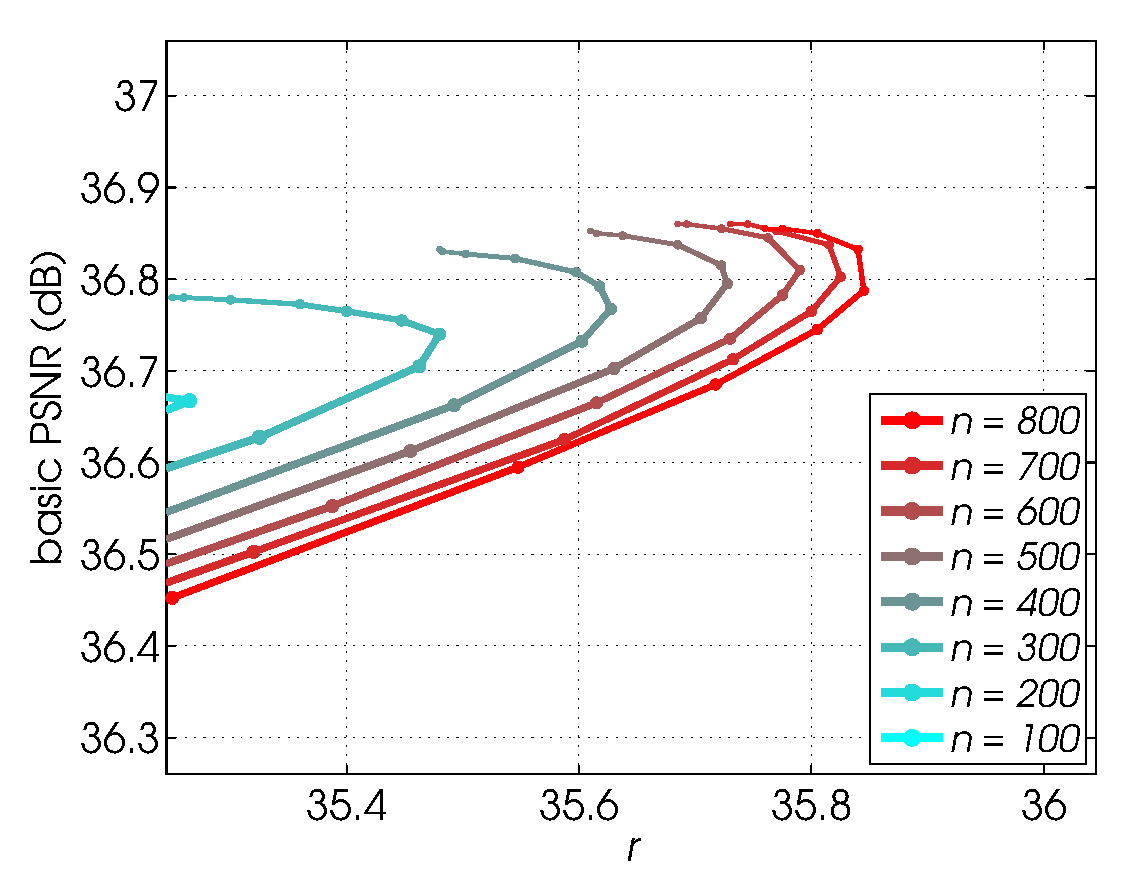
\includegraphics[width=.25\textwidth]{figs/params_tables/bpsnr-fpsnr_r1-np1-curves_s10_average_derf.eps}%
%-% 		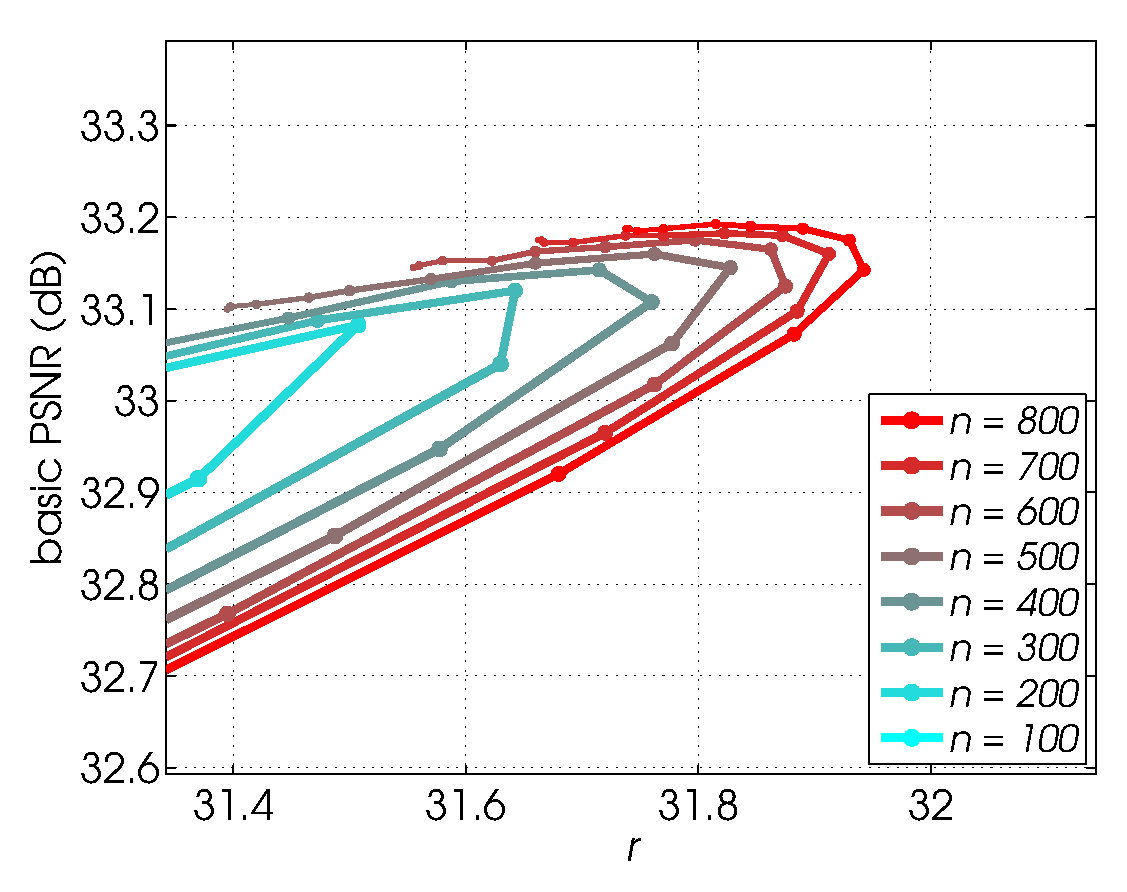
\includegraphics[width=.25\textwidth]{figs/params_tables/bpsnr-fpsnr_r1-np1-curves_s20_average_derf.eps}%
%-% 		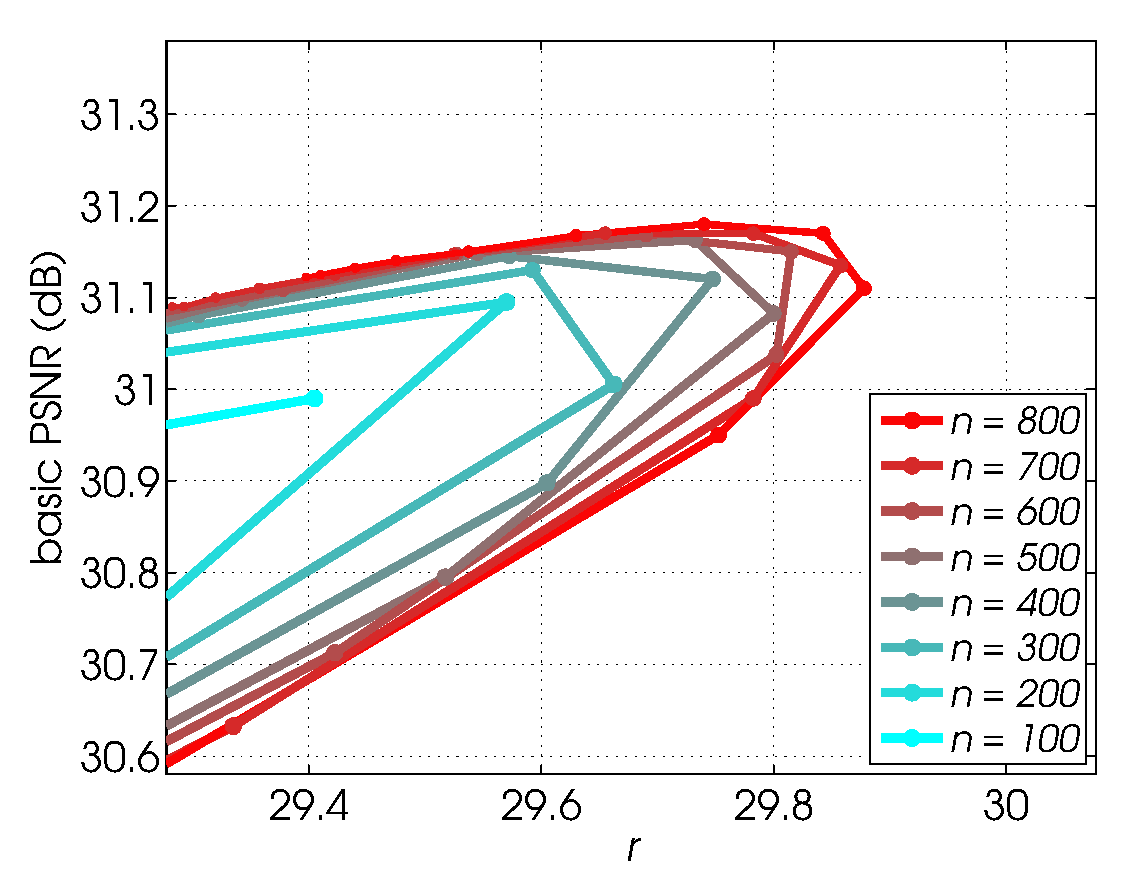
\includegraphics[width=.25\textwidth]{figs/params_tables/bpsnr-fpsnr_r1-np1-curves_s30_average_derf.eps}%
%-% 		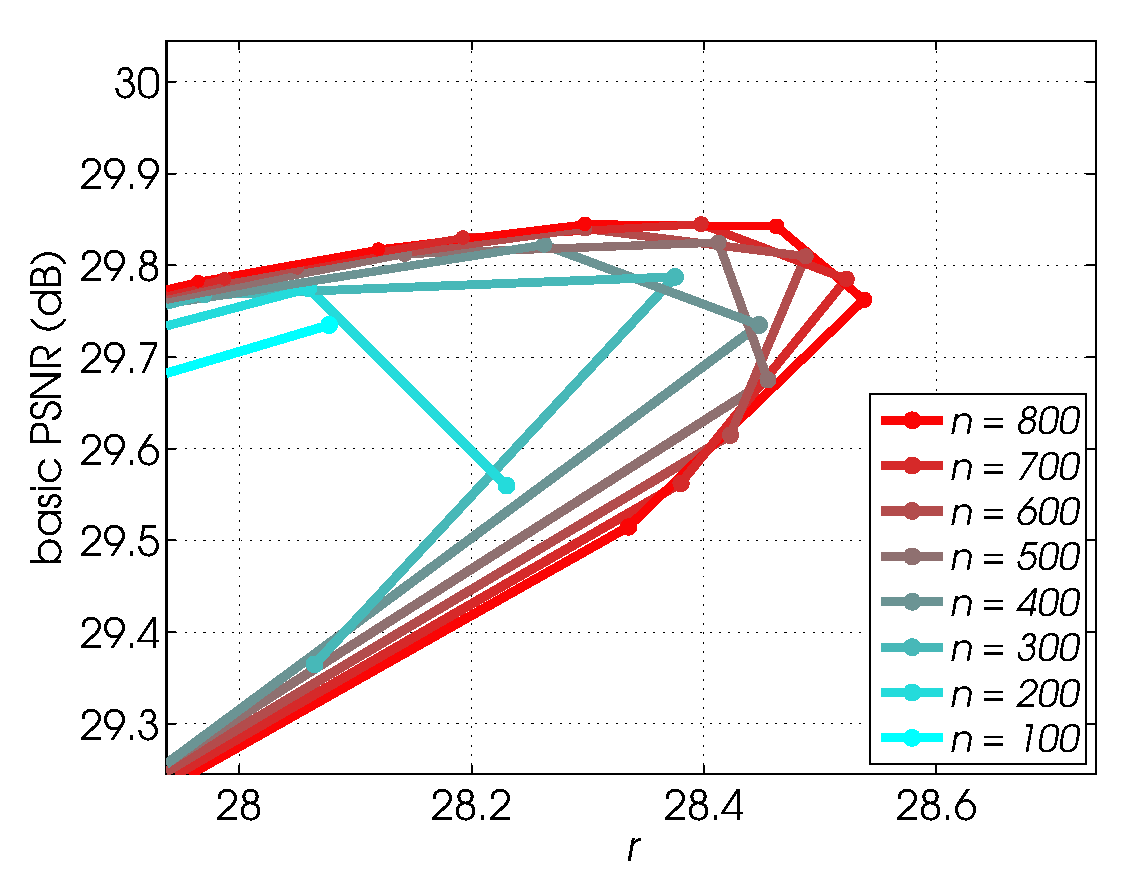
\includegraphics[width=.25\textwidth]{figs/params_tables/bpsnr-fpsnr_r1-np1-curves_s40_average_derf.eps}\\
%-% 
%-% 		\includegraphics[width=.25\textwidth]{figs/params_tables/bpsnr-fpsnr_r1-np1-curves_s10_average_mono.eps}%
%-% 		\includegraphics[width=.25\textwidth]{figs/params_tables/bpsnr-fpsnr_r1-np1-curves_s20_average_mono.eps}%
%-% 		\includegraphics[width=.25\textwidth]{figs/params_tables/bpsnr-fpsnr_r1-np1-curves_s30_average_mono.eps}%
%-% 		\includegraphics[width=.25\textwidth]{figs/params_tables/bpsnr-fpsnr_r1-np1-curves_s40_average_mono.eps}\\
%-% 	\end{center}
%-% 	\caption{PSNRs of final vs. basic estimate. Averages over four sequences, when varying the
%-% 		second stage parameters $r_1$ and $n_1$. From left to right, results for
%-% 		$\sigma = 10, 20, 30, 40$. Top: results for RGB sequences; bottom:
%-% 		results for grayscale sequences. The width of the line is proportional to
%-% 		the rank. \pcomment{These plots contradict the argument in favour of using
%-% 		full rank in the first stage (supposedly introducing a higher variance, but a
%-% 		smaller bias). It turns out, that (1) the final PSNR is pretty much
%-% 		correlated with the basic PSNR, and (2) the optimal rank for the final
%-% 		estimate is lower than that of the basic estimate. I do not have an explanation for this.}} 
%-% 	\label{fig:rank1-nsim1-bpsnr-fpsnr}
%-% \end{figure*}

\begin{figure*}[htpb!]
	\begin{center}
		\includegraphics[width=.25\textwidth]{figs/params_tables/fpsnr_r2-np2-curves_s10_average_derf_neg-weights.eps}%
		\includegraphics[width=.25\textwidth]{figs/params_tables/fpsnr_r2-np2-curves_s20_average_derf_neg-weights.eps}%
		\includegraphics[width=.25\textwidth]{figs/params_tables/fpsnr_r2-np2-curves_s30_average_derf_neg-weights.eps}%
		\includegraphics[width=.25\textwidth]{figs/params_tables/fpsnr_r2-np2-curves_s40_average_derf_neg-weights.eps}\\

		\includegraphics[width=.25\textwidth]{figs/params_tables/fpsnr_r2-np2-curves_s10_average_mono_neg-weights.eps}%
		\includegraphics[width=.25\textwidth]{figs/params_tables/fpsnr_r2-np2-curves_s20_average_mono_neg-weights.eps}%
		\includegraphics[width=.25\textwidth]{figs/params_tables/fpsnr_r2-np2-curves_s30_average_mono_neg-weights.eps}%
		\includegraphics[width=.25\textwidth]{figs/params_tables/fpsnr_r2-np2-curves_s40_average_mono_neg-weights.eps}\\

	\end{center}
	\caption{Final estimate PSNR, averaged over four sequences, when varying the
		second stage parameters $r_2$ and $n_2$. From left to right, results for
		$\sigma = 10, 20, 30, 40$. In the top row: results for RGB sequences, bottom
		row, results for grayscale sequences.} 
	\label{fig:rank2-nsim2-fpsnr}
\end{figure*}



%\begin{figure*}[htpb!]
%	\begin{center}
%		\includegraphics[width=.25\textwidth]{figs/params_tables/psnr_r2-np2-image_s10_average_derf.eps}%
%		\includegraphics[width=.25\textwidth]{figs/params_tables/psnr_r2-np2-image_s20_average_derf.eps}%
%		\includegraphics[width=.25\textwidth]{figs/params_tables/psnr_r2-np2-image_s40_average_derf.eps}\\
%		\includegraphics[width=.25\textwidth]{figs/params_tables/time_r2-np2-image_s10_average_derf.eps}%
%		\includegraphics[width=.25\textwidth]{figs/params_tables/time_r2-np2-image_s20_average_derf.eps}%
%		\includegraphics[width=.25\textwidth]{figs/params_tables/time_r2-np2-image_s40_average_derf.eps}\\
%	\end{center}
%	\caption{Top row: average PSNRs over four sequences, obtained by varying the second stage parameters
%		$r$ and $n$. From left to right, results for $\sigma = 10,
%		20, 40$. In each image, the contrast has been stretched so that white
%		corresponds to the maximum PSNR and black to a decay of 1dB bellow the
%		maximum. 
%		Bottom: corresponding average running times. White corresponds to $50$ s/frame (using parallelization with four threads).}
%	\label{fig:rank-nsim-image-stage2}
%\end{figure*}
%
%
%\begin{figure*}[htpb!]
%	\begin{center}
%		\includegraphics[width=.25\textwidth]{figs/params_tables/psnr_r1-np1-image_s10_average_derf.eps}%
%		\includegraphics[width=.25\textwidth]{figs/params_tables/psnr_r1-np1-image_s20_average_derf.eps}%
%		\includegraphics[width=.25\textwidth]{figs/params_tables/psnr_r1-np1-image_s40_average_derf.eps}\\
%		\includegraphics[width=.25\textwidth]{figs/params_tables/time_r1-np1-image_s10_average_derf.eps}%
%		\includegraphics[width=.25\textwidth]{figs/params_tables/time_r1-np1-image_s20_average_derf.eps}%
%		\includegraphics[width=.25\textwidth]{figs/params_tables/time_r1-np1-image_s40_average_derf.eps}\\
%	\end{center}
%	\caption{Same as Figure \ref{fig:rank-nsim-image-stage2} but for the first stage.}
%	\label{fig:rank-nsim-image-stage1}
%\end{figure*}


%\begin{figure*}[htpb!]
%	\begin{center}
%		\includegraphics[width=.25\textwidth,height=.19\textwidth]{figs/params_tables/zoom_psnr_px1-np1-bars_1r8_s10_average.eps}%
%		\includegraphics[width=.25\textwidth,height=.19\textwidth]{figs/params_tables/zoom_psnr_px1-np1-bars_1r16_s10_average.eps}%
%		\includegraphics[width=.25\textwidth,height=.19\textwidth]{figs/params_tables/zoom_psnr_px1-np1-bars_1r32_s10_average.eps}%
%		\includegraphics[width=.25\textwidth,height=.19\textwidth]{figs/params_tables/zoom_psnr_px1-np1-bars_1r64_s10_average.eps}\\
%		\includegraphics[width=.25\textwidth,height=.19\textwidth]{figs/params_tables/zoom_psnr_px1-np1-bars_1r8_s20_average.eps}%
%		\includegraphics[width=.25\textwidth,height=.19\textwidth]{figs/params_tables/zoom_psnr_px1-np1-bars_1r16_s20_average.eps}%
%		\includegraphics[width=.25\textwidth,height=.19\textwidth]{figs/params_tables/zoom_psnr_px1-np1-bars_1r32_s20_average.eps}%
%		\includegraphics[width=.25\textwidth,height=.19\textwidth]{figs/params_tables/zoom_psnr_px1-np1-bars_1r64_s20_average.eps}\\
%		\includegraphics[width=.25\textwidth,height=.19\textwidth]{figs/params_tables/zoom_psnr_px1-np1-bars_1r8_s40_average.eps}%
%		\includegraphics[width=.25\textwidth,height=.19\textwidth]{figs/params_tables/zoom_psnr_px1-np1-bars_1r16_s40_average.eps}%
%		\includegraphics[width=.25\textwidth,height=.19\textwidth]{figs/params_tables/zoom_psnr_px1-np1-bars_1r32_s40_average.eps}%
%		\includegraphics[width=.25\textwidth,height=.19\textwidth]{figs/params_tables/zoom_psnr_px1-np1-bars_1r64_s40_average.eps}\\
%	\end{center}
%	\caption{Average PSNRs for 64 configurations of the first stage parameters
%		$r$, $n$ and $s_x$. From top to bottom, results for $\sigma = 10, 20, 40$.
%		From left to right: results for $r = 8, 16, 32, 64$.}
%	\label{fig:rank-px-nsim-table-stage1}
%\end{figure*}
%
%\begin{figure*}[htpb!]
%	\begin{center}
%		\includegraphics[width=.25\textwidth,height=.19\textwidth]{figs/params_tables/zoom_psnr_px2-np2-bars_2r8_s10_average.eps}%
%		\includegraphics[width=.25\textwidth,height=.19\textwidth]{figs/params_tables/zoom_psnr_px2-np2-bars_2r16_s10_average.eps}%
%		\includegraphics[width=.25\textwidth,height=.19\textwidth]{figs/params_tables/zoom_psnr_px2-np2-bars_2r32_s10_average.eps}%
%		\includegraphics[width=.25\textwidth,height=.19\textwidth]{figs/params_tables/zoom_psnr_px2-np2-bars_2r64_s10_average.eps}\\
%		\includegraphics[width=.25\textwidth,height=.19\textwidth]{figs/params_tables/zoom_psnr_px2-np2-bars_2r8_s20_average.eps}%
%		\includegraphics[width=.25\textwidth,height=.19\textwidth]{figs/params_tables/zoom_psnr_px2-np2-bars_2r16_s20_average.eps}%
%		\includegraphics[width=.25\textwidth,height=.19\textwidth]{figs/params_tables/zoom_psnr_px2-np2-bars_2r32_s20_average.eps}%
%		\includegraphics[width=.25\textwidth,height=.19\textwidth]{figs/params_tables/zoom_psnr_px2-np2-bars_2r64_s20_average.eps}\\
%		\includegraphics[width=.25\textwidth,height=.19\textwidth]{figs/params_tables/zoom_psnr_px2-np2-bars_2r8_s40_average.eps}%
%		\includegraphics[width=.25\textwidth,height=.19\textwidth]{figs/params_tables/zoom_psnr_px2-np2-bars_2r16_s40_average.eps}%
%		\includegraphics[width=.25\textwidth,height=.19\textwidth]{figs/params_tables/zoom_psnr_px2-np2-bars_2r32_s40_average.eps}%
%		\includegraphics[width=.25\textwidth,height=.19\textwidth]{figs/params_tables/zoom_psnr_px2-np2-bars_2r64_s40_average.eps}\\
%	\end{center}
%	\caption{Average PSNRs for 64 configurations of the second stage parameters
%		$r$, $n$ and $s_x$. From top to bottom, results for $\sigma = 10, 20, 40$.
%		From left to right: results for $r = 8, 16, 32, 64$.}
%	\label{fig:rank-px-nsim-table-stage2}
%\end{figure*}



\subsection{Search region and patch size}

Setting the size of the search region implies a trade-off between denoising
performance and running time: A larger search region takes longer to traverse
but yields better results, since more similar patches can be found. We use the same 
search region in both stages. The
temporal search window is fixed at $w_t = 5$. The spatial search region is set at
$w_x = 37$ for color videos and $w_x = 45$ for grayscale videos.
With these values, the search region captures the $5$ frame trajectory of the
target patch as long as it moves slower than $37/5 = 7.4$ pixels/frame (for
color videos).

Let us now consider the spatial patch
size $s_x$, which is a key parameter in patch-based methods \cite{Buades2006,Kervrann2006,Boulanger2007}.
%The distribution of the 
%patch distances is a non-central Chi-squared distribution \cite{Dabov2007tip}
%\pcomment{CHECK!}
%with variance 
%\[\textnormal{Var}\left\{\frac1{m}\|\ma q_1 - \ma q_2\|^2\right\} = \frac{8\sigma^2}{m}\left(\sigma^2 + \frac{\|\ma p_1 - \ma p_2\|^2}{m}\right),\]
%where $m = s_x^2s_t$ is the total number of pixels in the patch.
%*% Increasing the spatial patch size $s_x$ reduces the variance of the noise in the patch
%*% distance. 
%*% However, for larger
%*% patches it becomes less likely to find other patches with a similar texture
%*% pattern. The use spatio-temporal patches helps in solving this trade-off: for
%*% instance, with a spatio-temporal patch of size $5\times 5\times 4$, we obtain
%*% the same patch distance noise as with a spatial patch of size $10\times 10
%*% \times 1$. Moreover, as discussed in \S \ref{sse:spatio-temporal-patches}, for
%*% an approximately uniform motion, the 
%*% amount of similar neighbors of a $5\times 5\times 4$ patch is roughly the same
%*% as for a $5\times 5\times 1$ patch.
%
For color videos, we will set the spatial patch size at $s_x = 5$ for both
stages, whereas for grayscale videos we use $s_x = 7$. Larger patches (up to $s_x = 9$) lead to an mild improvement of the
results (on average). This improvement comes at a considerable increase in the
computation time, since our current implementation is $\mathcal O(s_x^4)$.
Thus, have found that a good compromise between computation time and quality is
given by $s_x = 5$.

The impact of the temporal patch size $s_t$ will be discussed later in Section
\ref{sec:results}, where we show results varying $s_t$ between $s_t = 1$ and $s_t = 4$.

\subsection{Rank and number of similar patches}

The number of similar patches $n$ and the rank $r$ affect the estimation of the covariance
matrix $C$, controlling the trade-off between the accuracy of the Gaussian model
and the precision of the covariance matrix,
which in turn has a direct effect on the denoising strength of the algorithm.
% This have great impact on the bias-variance trade-off of the denoiser.
%In practice, these parameters determine the denoising strength of the
%algorithm. For example, using a large
We found a compromise to this trade-off empirically, by trying different values
of this parameter on a few training sequences and keeping the one that yields
the best PSNR on average.

%The number of similar patches $n$ and the rank $r$ affect the estimation of the covariance
%matrix $C$, controlling the trade-off between the accuracy of Gaussian model
%and precision of the covariance matrix.


%\prm{Intuitively speaking, by setting a lower rank we are estimating a covariance
%matrix in a lower dimensional subspace. Then, according to
%\cite{Vershynin2012}, we require a smaller number of samples for a given
%precision.} \pcomment{The previous argument is not good. I would like to have
%some theoretical estimate on the number of samples to approximate a lower
%rank covariance matrix, or equivalently, the number of samples to approximate
%the largest principal directions. The point I would like to make, is that
%the number of similar patches required is less if one only wants to estimate
%the first principal eigenvectors. Maybe the answer lies in \cite{Halko2011}.}

The plots in Figure \ref{fig:rank1-nsim1-psnr-color} show the PSNRs of the
basic and final estimates as a function of the rank $r_1$, for several values
of $n_{1}$. The curves correspond to an average over 20 frames clips extracted
from four classical test color sequences, namely \emph{bus}, \emph{foreman},
\emph{football} and
\emph{tennis}. The sequences were contaminated with
AGWN of standard deviation $\sigma = 10, 20, 30, 40$. 
Figure \ref{fig:rank1-nsim1-psnr-gray} shows the results for a
grayscale version of the same sequences. 
%
%

\padd{For the basic estimate, we show two set of curves. The dashed curves were
obtained by zeroing out negative eigenvalues of the estimated a priori covariance
matrix $\widehat C$, computed according to \eqref{eq:learn_parameters}. The continuous curves 
were obtained by retaining negative eigenvalues. In this case the MAP is estimated
with an empirical Wiener filter that may have some negative coefficients.}

\padd{For lower values of the rank parameter $r$, both curves coincide, since the first
eigenvalues are positive. 
For all noise levels, all curves of fixed $n_1$ present a first peak at a low value of the rank $r$.
The behaviour of the basic estimate around this peak can be
interpreted in the light of the theoretical results described in \S
\ref{sse:covariance-estimation}.
As the noise level increases, the rank at which the peak is attained
shifts to the left. This makes sense, as the reliability of the computed eigenvectors
decrease with increasing noise.
%
Also, for a fixed noise level, when the number of samples $n_1$ increases, the value
of the peak increases also, and so does the rank at which it is attained.
This is again explainable, as smaller groups obtained by keeping only the
most similar patches have less modes of variation, and thus a worse signal-to-noise ratio
in the eigenvectors with lower eigenvalues.}
%As the group of patches grows
%bigger, patches in the group are not as similar anymore, and a higher rank is
%needed to allow for additional modes of variation.

%The eigenvalues of $\widehat C$ are given by $\hat \lambda_i = \widehat \nu_i -
%\sigma^2$, where $\widehat \nu_i$ are the eigenvalues of the empirical
%\emph{a posteriori} covariance matrix.
%In practice due to the estimation errors, several
%$\widehat \nu_i$ are smaller than $\sigma^2$. These translate into negative
%coefficients $w_{ii}$ in the empirical Wiener filter \eqref{eq:wiener_coeffs},
%which result in a poorer estimation of the MAP.
\padd{As the rank parameter increases, both curves diverge. 
The dashed curves become almost constant at the point when
most eigenvalues become negative. After that point increasing the
rank has no effect if the negative eigenvalues are zeroed out.
%
Surprisingly, these negative coefficients have a positive effect on the final 
result, creating the second peak for high values of the rank shown by the
continuous plots. Currently we do not have an explanation for this behaviour
although it is related to the aggregation: even if the estimated MAP for the
patches in each group have larger errors, after aggregation these errors seem
to cancel, yielding an overall better estimate of the clean image.}

\padd{The final estimate shows the same qualitative behaviour with respect to the first
stage parameters. The dashed curves obtained by zeroing out the negative
eigenvalues are not shown to avoid cluttering the figure. Essentially the
second step has the effect of reducing the differences between results obtained
with different parameters. Based on these curves, we fix the first stage parameters at
$n_1 = 300$ and $r_1 = 95$ for color videos, and at $n_1 = 300$ and $r_1 = 180$ for grayscale videos.}

Using these parameters for the first stage, we analyzed the impact when varying the second stage
parameters $n_2$ and $r_2$. The plots obtained are shown in Figure
\ref{fig:rank2-nsim2-fpsnr}.
%
Note that in this case, the \emph{a
priori} covariance matrix is estimated from the basic estimate (without having
to subtract $\sigma^2I$). As a consequence, the are no negative filter coefficients.
%
In the second stage the quality drops when
using a number of patches $n_2$ higher than $100$. This differs from the first stage,
where a larger $n_1$ yielded a better PSNR.
The reason for this lies probably in the fact that the patches have less noise,
and a good estimate of the leading eigenvectors of the covariance matrix can be obtained
with less patches. Furthermore, smaller groups of patches
are better modelled by a Gaussian distribution.
%\pcomment{I don't have an explanation for the curves for $\sigma = 10$. Precisely
%in the lower noise level, the PSNR drops when $n_2$ is reduced, except for lower ranks.
%This contradicts the argument given: for less noise, it should be always better to consider
%less patches, not only for lower ranks.} 
Based on these plots, we set the following values for the parameters
\[r_2(\sigma) = 30 - \frac12(\sigma - 10),\quad\quad n_{2} = 100.\]

All parameters are summarized in Table \ref{tab:parameters}.

%Note that due to the coupling of the first and second stages, determining the
%optimal values for the ranks $r_1, r_2$ and the number of patches $n_1,n_2$
%would require a four dimensional parameter search which would be to costly.
%
%Instead, we fixed the first stage parameters, both for color and grayscale videos
%at
%\[r_1 = s_{x,1}^2s_{t,1}\quad\quad n_{1} = 400,\]
%which we found to give good results. In doing so, we were conservative and
%used the full rank covariance matrix to eliminate the least signal components.
%%
%We then ran a parameter search to determine $r_2$ and $n_{2}$.
%The results are the ones shown in Figure \ref{fig:rank1-nsim1-psnr-gray}. This led
%us to establish the following values as a function of $\sigma$:
%%\[r_2(\sigma) = 40 - \frac13(\sigma - 10)\quad\quad n_{2} = 150.\]
%\[r_2(\sigma) = 35 - \frac12(\sigma - 10)\quad\quad n_{2} = 100.\]
%The same values are used for color and grayscale videos.
%Note that a higher value for $n_{2}$ would give slightly worse results,
%at a lower computational cost.


\begin{table}
	\centering
	\begin{tabular}{l | c c | c c }
		& \multicolumn{2}{c|}{color} 
		& \multicolumn{2}{c}{grayscale}\\
		Stage                            & 1st    & 2nd   & 1st   & 2nd   \\\hline\hline
		$s_x$        &  5 & 5 & 7 & 7 \\
		$s_t$        &  1--4  & 1--4  & 1--4  & 1--4  \\
		$w_x$        &  37    & 37    & 45    & 45    \\
		$w_x$        &   5    & 5     & 5     & 5    \\
		$n$          & 300    & 100   & 300   & 100  \\
		$r$          & 95   & $30 - \frac12(\sigma - 10)$    & 180  & $30 - \frac12(\sigma - 10)$   \\
%		Distance threshold $\tau$   & n/a  & 432  & n/a  & 432  & n/a  & 432 \\
%		Beta                        & 1    & 1.2  & 1    & 1.2  & 1    & 1.2 \\\hline
	\end{tabular}
	\caption{Selected parameters.}
	\label{tab:parameters}
\end{table}


%Intuitively, smaller groups obtained by keeping only the most similar patches have 
%only a few modes of variation and thus are better modelled with a low rank
%covariance matrix. As the group of patches grows bigger, patches in the group
%are not as similar anymore, and a higher rank is needed to model these additional 
%variation.
%To find appropriate values for these parameters, we compute denoising results
%varying the rank $r$ and the number of similar patches $n$, while
%keeping all other parameters fixed. Results are computed for four 20 frames clips
%extracted from the sequences \emph{bus}, \emph{foreman}, \emph{football} and
%\emph{tennis}, adding noise of $\sigma = 10, 20, 40$.
%%
%We do this for each stage, starting by the second.
%
%On this first experiment, the parameters of the first stage are fixed at:
%\[w_x = 37,\,\,w_t = 5\,\,s_x = 5,\,\,s_t = 4,\,\,n = 375,\,\,r = 100.\]
%\todo{Check these parameters}
%Note that $r = 100$ is the full rank.
%For the second stage, we fix $w_x = 37$, $w_t = 5$, $s_x = 5$ and $s_t = 3$, while varying 
%$r$ in $10,20,\dots,80$ and $n$ in $50, 150,200,250$.
%The results can be visualized in Figure \ref{fig:rank-nsim-image-stage2}. The images in the 
%figure show the PSNR loss in dB with respect to the maximum value attained at each noise level.
%White means 0dB (\ie the set of parameters where the maximum was attained) and black means a loss
%greater or equal than 1dB.
%
%We can observe that, at constant $n$ there is an optimal value for the rank. Bellow
%these value the PSNR drops sharply, and above it, the decay is slower. The
%optimal rank for a given $n$ increases with $n$ and decreases with $\sigma$.
%Best results are obtained for small $n$. However, this also entails a higher running time, 
%since it increases the number of groups of similar patches that need to be
%processed. We found a good compromise by setting $n = 150$ and $r$ as a decreasing function of $\sigma$:
%\[r(\sigma) = 40 - \frac1{10}(\sigma - 40),\]
%which corresponds to a line through $(s=10, r = 40)$ and $(s=40, r = 30)$.
%
%We now perform a similar search for the first stage, setting the second step parameters as:
%\[w_x = 37,\,\,w_t = 5\,\,s_x = 5,\,\,s_t = 3,\,\,n = 150,\,\,r(\sigma).\]
%The first stage parameters are as before, expect that we now vary $r$ in $10,20,\dots,100$
%and $n$ in $50,100,\dots,650$. Results are shown in Figure
%\ref{fig:rank-nsim-image-stage1}. Note that since our objective is to maximize
%the final PSNR, we show here the final PSNR. 
%The final and the basic PSNRs do not always
%have the same behaviour. Improving the basic PSNR does not always lead to an
%improvement in the final one. The reason for this is that it is preferable to
%apply a conservative noise reduction leaving some noise in the basic estimate
%(high variance but small bias). In the second step, this residual noise has
%little effect on the estimation of the patch distances and the \emph{a priori} covariance
%matrix. On the other hand, applying a more aggressive denoising in first step
%might increase the basic PSNR, but the second step cannot recover the lost
%signal components.
%
%In fact, best results are obtained using the full rank covariance matrix. 
%In accordance to these observations, we will set the first values for $r$ and $n$ as:
%\begin{equation}
%	r = s_x^2s_t \quad\quad n = 350.
%	\label{eq:stage1_parameters}
%\end{equation}

%
%
%
%First we fix the parameters of the second stage at 
%\[r = 16,\,\, n = 160,\,\, s_x = 5,\,\, s_t = 3,\,\, w_x = 37,\,\, w_t = 5,\]
%and vary the parameters of the first stage. We considered ranks $r = 8, 16, 32, 64$,   
%patch sizes $s_x = 3,5,7,9$ and number of patches $n = 80, 160, 320, 640$.
%For all $4^3 = 64$ combinations, we considered three levels of noise $\sigma = 10, 20, 40$
%and run our method on four sequences. The
%sequences used were \emph{army, dog dance, evergreen} and \emph{walking} from
%the Middlebury optical flow benchmark \cite{middleburyOflow}.
%The sequences have 8 frames of size $584 \times 388$ (\emph{army}) and $640
%\times 480$ (\emph{dog dance, evergreen} and \emph{walking}).
%These sequences were chosen to have some variety of motions, textures, etc.
%
%Figure \ref{fig:rank-px-nsim-table-stage1} shows for each configuration of
%parameters and level of noise, the average PSNR over the four sequences. The
%cyan bars correspond to the basic estimate and the ones in magenta to the final
%estimate.
%
%It can be observed that several parameter configurations can give very similar
%results. For example, with $\sigma = 10$, equivalent results can be obtained 
%with $s_x = 3, r = 16, n = 80$, $s_x = 5, r = 32, n = 160$
%or  $s_x = 7, r = 64, n = 320$.
%The one with the least computational cost is chosen. This means,
%smaller patches sizes, smaller ranks, and a larger number of similar patches.
%
%Another thing to notice is that the final and the basic PSNRs do not always
%have the same behaviour. Improving the basic PSNR does not always lead to an
%improvement in the final one. The reason for this is that it is preferable to
%apply a conservative noise reduction leaving some noise in the basic estimate
%(high variance but small bias). In the second step, this residual noise has
%little effect on the estimation of the patch distances and the \emph{a priori} covariance
%matrix. On the other hand, applying a more aggressive denoising in first step
%might increase the basic PSNR, but the second step cannot recover the lost
%signal components.
%
%The strength of the denoising is controlled through the rank and the number of
%patches in the group. For lower levels of noise, \ie $\sigma = 10$, better
%PSRNs can be achieved with a higher rank and using a smaller number of similar
%patches. When increasing the noise, the rank should be decreased and the number 
%of similar patches increased.
%
%In accordance to these observations, we will set the parameters as a function of
%$\sigma$ as follows:
%\begin{equation}
%	s_t = 5,\quad\quad r = \min(640/\sigma, r_{\text{max}}), \quad\quad n = 16\sigma.
%	\label{eq:stage1_parameters}
%\end{equation}
%%\begin{align}
%%	s_t &= 5\\
%%	r &= \min(640/\sigma, r_{\text{max}}) \\
%%	n &= 16\sigma. 
%%	\label{eq:stage1_parameters}
%%\end{align}
%We set the maximum rank to be $r_{\text{max}} = \min(128,s_x^2s_t)$. Note that
%$r = s_x^2s_t$ corresponds to the full rank.
%
%We now search for the optimum parameters for the second stage, setting the 
%first stage parameters according to \eqref{eq:stage1_parameters}. The temporal
%patch size is again set as $s_t = 3$ for both stages and the search regions are
%kept as in \eqref{eq:search_region_parameters}. Figure
%\ref{fig:rank-px-nsim-table-stage2} shows the average PSNRs over the four
%sequences, obtained for each parameter configuration and each noise level.
%
%From these results, we fix the parameters as follows:
%\begin{equation}
%	s_x = 5,\quad r = \max( \min(320/\sigma, r_{\text{max}}), r_{\text{min}}), \quad n = 160.
%	\label{eq:stage1_parameters}
%\end{equation}
%For the second stage, we set $r_{\text{max}} = \min(64,s_x^2s_t)$ and $r_{\text{min}} = 16$.




%We will fix the temporal size and for the
%temporal size of the patch we will vary it between $s_t = 1$ and $s_t = 4$ in
%the results section.




%For the experiments shown in \S \ref{sec:results} we used the following 
%parameters.
%\begin{LaTeXdescription}
%	\item[Patch size:] In both stages, we fixed the patch size at $s = 5$. Better 
%		results can be obtained with higher patch sizes, but the computational cost
%		scales considerably (e.g. the inversion of the covariance matrix is of $O(s^6)$).
%	\item[Number of similar patches:] For the first stage, we set
%		$N^{(1)}_{\text{sim}} = 3s^2w_t$  (recall that $w_t$ is the temporal
%		extend of the search region). For the second step we 
%		found better results using fewer patches, thus we set $N^{(2)}_{\text{sim}} = 3/4 s^2w_t$.
%	\item[Search region:] In both stages, we used $w_x = s^2/2$.
%		For the temporal search region, we found a good trade-off
%		between computational time and quality of the results for $w_t = 5$. 
%	\item[Patch distance threshold:] When building the group of similar patches
%		in the second stage, more than $n$ patches are allowed if their 
%		distances with respect to the reference patch are smaller than a threshold $\tau$.
%		As in \cite{Lebrun2013ipol}, we set $\tau = 4$ (the distance between patches is normalized by 
%		the number of elements in the patch and the number of channels).
%\end{LaTeXdescription}

% stage 1
%
% patch size $s = 5$
% spatial search region $w_x = 37$
% temporal search region $w_t = 0,3,5$
% number of similar patches $3 s^2 w_t$, 3/4 s^2 w_t$$
% beta $\beta = 1; 1.2$
% tau n/a $\tau = 16$  
% offset $= s/2$

% stage 2
%
% patch size 
% spatial search region
% temporal search region
% number of similar patches
% beta
% tau
% offset


\section{Results}
\label{sec:results}

In this section we present results obtained with the proposed
method on some classical test sequences with Gaussian noise added.
We consider separately the cases of grayscale and color videos.
All results were computed with the parameters shown in Table \ref{tab:parameters}.
The actual sequences can be downloaded from the project's
website\footnote{\url{http://dev.ipol.im/~pariasm/video_nlbayes/}} in uncompressed format.


\subsection{Results on grayscale videos}

We present denoising results on six classic test sequences used commonly in the
literature. We compared against two state-of-the-art methods: V-BM4D
\cite{Maggioni2012}, and the method of Li, Zhang and Dai \cite{LiZhangDai2011}
which we call I-SA-BM4D, since it can be regarded as an iterative version of BM4D \cite{Maggioni2013}
using shape adaptive 3D patches, as in \cite{Ercole2005}.  
For V-BM4D, we show results corresponding to two
different choices of parameters. The method labeled V-BM4D-tip
corresponds to the results reported
in \cite{Maggioni2012}. The results labeled V-BM4D-mp were
obtained using the implementation available online \cite{bm4dcode}. This
implementation provides three parameter profiles of increasing quality and
complexity: ``low complexity profile'', ``normal profile'' and ``modified
profile''. We show the results obtained with the modified profile.

Each sequence was contaminated with AGWN of $\sigma =
10,20,30,40$. Table \ref{tab:psnr-classic-gray} shows the
PSNR values obtained after denoising. For our method, we show results varying the temporal
component of the patch size between $s_t = 1$ (2D patch) and $s_t = 4$ frames.
For our method and V-BM4D-mp we show the PSNR of the basic estimate as well.

The best results by a large margin are the ones reported in
\cite{LiZhangDai2011}. This method builds uppon BM4D, which in \cite{Maggioni2013}
is applied to volumetric imagery. The authors explored its applicability to video 
and the results show that it is inferior to V-BM4D, at least 
for low to moderate noise levels. The method of Li, Zhang and Dai \cite{LiZhangDai2011} 
considers shape adaptive patches, and performs several iterations. In each iteration,
the previous iterate is used as an oracle to compute patch distances.
\padd{An additional difference is that the oracle is not used to determine the
signal components for the Wiener filter. Instead, these are estimated with a fixed
point iteration from the original noisy patches.}

We can see that our results outperform the ones of V-BM4D, for all sequences and 
for all noise levels. The results reported by \cite{LiZhangDai2011} show that there
is still room for improvement (albeit perhaps at a higher computational cost).
%
We have attempted iterating our method as in \cite{LiZhangDai2011},
but we have not found yet a significant improvement. Something similar was
reported in \cite{Lebrun2013ipol,Lebrun2013a} for the NL-Bayes method in still
images. %It may be that the current parameters are not suitable for
%iteration. 
A more systematic study is has to be conducted before drawing any
conclusions about iterative versions of the algorithm.
%This is the matter of ongoing work, but is out of the scope of the paper.
%Still, it is early to exclude iteration as an valid option to
%further improve the denoising performance.

For a qualitative comparison, Figure \ref{fig:results_mobile_mono}
shows two details of the results obtained by our method and V-BM4D for the
\emph{mobile} sequence, for noise of $\sigma = 10, 20, 40$. It can be observed
that the proposed method preserves the fine details betters, such as the thin
lines of the drawing in the first example, or the calendar numbers in the
second example. It also exhibits a higher temporal consistency, as will be
shown in \S \ref{sse:temporal-consistency}.


Regarding the running time, let us note that the modified profile has a
computation time lower to that of our method. Running with a
single core in an Intel Xeon X7560 (2.27GHz) CPU, 
our current implementation takes on average $XXs$ per frame for a video of CIF
resolution ($352\times288$). V-BM4D takes $44s$ with the modified profile.
The running times of \cite{LiZhangDai2011} are not reported, but we expect them
to be significantly higher given that the algorithm is iterative, with each iteration 
being comparable to one of the stages of V-BM4D.
\pcomment{TODO: Compute running times!!!}
\pcomment{We should include computation times for grayscale videos, instead of color}

\begin{table*}[htp!]
	\begin{center}
		{\small
		\renewcommand{\tabcolsep}{1.6mm}
		\renewcommand{\arraystretch}{1.3}
		\begin{tabular}{ c | l |c c | c c | c c | c c | c c | c}
			\hline
			\rule{0pt}{10pt}$\sigma$ & Method            & \multicolumn{2}{c}{Tennis}  & \multicolumn{2}{c}{Coastguard}&\multicolumn{2}{c}{Foreman}& \multicolumn{2}{c}{Bus}     &\multicolumn{2}{c|}{Football}& Average\\\hline
			\multirow{1}{*}{$ 5$}
%			                      & CIFIC                & \bsic{     } &              & \bsic{     } &              & \bsic{     } &              & \bsic{     } &              & \bsic{     } &              &              \\
			                      & V-BM3D               & \bsic{     } &       39.45  & \bsic{     } &       40.18  & \bsic{     } &       40.16  & \bsic{     } &       39.07  & \bsic{     } &              &       39.71  \\
			                      & V-BM4D-tip           & \bsic{     } & \best{39.98} & \bsic{     } & \best{41.13} & \bsic{     } & \best{41.38} & \bsic{     } & \best{40.21} & \bsic{     } & \best{     } & \best{40.68} \\
			                      & V-BM4D-mp            & \bsic{39.61} &       39.60  & \bsic{40.20} &       40.28  & \bsic{40.73} &       40.78  & \bsic{39.45} &       39.56  & \bsic{39.91} &       40.00  &       40.06  \\
			                      & VNLB   $s_t = 1$     & \bsic{38.83} &       39.37  & \bsic{41.05} &       41.49  & \bsic{41.41} &       41.95  & \bsic{40.05} &       40.43  & \bsic{41.30} &       41.75  &       40.81  \\
			                      & VNLB   $s_t = 2$     & \bsic{39.70} & \Best{40.15} & \bsic{41.76} &       42.25  & \bsic{42.01} & \Best{42.56} & \bsic{40.33} &       40.97  & \bsic{41.50} & \Best{41.97} &       41.48  \\
			                      & VNLB   $s_t = 3$     & \bsic{40.00} & \Best{40.16} & \Bsic{41.94} & \Best{42.45} & \Bsic{42.14} & \Best{42.61} & \Bsic{40.43} & \Best{41.12} & \Bsic{41.50} & \Best{41.85} & \Best{41.59} \\
			                      & VNLB   $s_t = 4$     & \Bsic{40.11} &      {40.01} & \Bsic{41.95} & \Best{42.38} & \Bsic{42.15} &       42.48  & \Bsic{40.47} &       41.02  & \Bsic{41.44} &      {41.61} &       41.47  \\\hline
%			                      & VNLB   $s_t = 1$     & \bsic{38.73} &       39.26  & \bsic{40.90} &       41.38  & \bsic{41.19} &       41.82  & \bsic{39.85} &       40.32  & \bsic{41.10} &       41.64  & \bsic{todo } &       todo   \\
%			                      & VNLB   $s_t = 2$     & \bsic{39.56} &       40.05  & \bsic{41.61} &       42.08  & \bsic{41.75} &       42.42  & \bsic{40.10} &       40.73  & \bsic{41.29} &       41.88  & \bsic{todo } &       todo   \\
%			                      & VNLB   $s_t = 3$     & \bsic{39.82} &       40.16  & \Bsic{41.75} &       42.39  & \Bsic{41.85} &       42.57  & \Bsic{40.16} &       40.96  & \Bsic{41.27} &       41.85  & \Bsic{todo } &       todo   \\
%			                      & VNLB   $s_t = 4$     & \Bsic{39.92} & \Best{40.03} & \Bsic{41.76} & \Best{42.41} & \Bsic{41.84} & \Best{42.48} & \Bsic{40.18} & \Best{40.92} & \Bsic{41.23} & \Best{41.67} & \Bsic{todo } & \Best{todo } \\\hline
%
			\multirow{1}{*}{$10$}
%			                      & CIFIC                & \bsic{     } &              & \bsic{     } &              & \bsic{     } &              & \bsic{     } &              & \bsic{     } &              &              \\
			                      & V-BM3D               & \bsic{     } &       36.04  & \bsic{     } &       36.82  & \bsic{     } &       37.52  & \bsic{     } &       34.96  & \bsic{     } &              &       36.34  \\
			                      & V-BM4D-tip           & \bsic{     } & \best{36.42} & \bsic{     } & \best{37.27} & \bsic{     } &       37.92  & \bsic{     } &       36.23  & \bsic{     } &              &       36.96  \\
			                      & V-BM4D-mp            & \bsic{35.64} &       35.90  & \bsic{36.06} &       36.30  & \bsic{36.96} &       37.21  & \bsic{35.10} &       35.38  & \bsic{35.79} &       36.08  &       36.20  \\
			                      & VNLB   $s_t = 1$     & \bsic{34.67} &       35.30  & \bsic{36.95} &       37.30  & \bsic{37.47} &       38.16  & \bsic{35.81} &       36.38  & \bsic{37.17} &       37.81  &       36.78  \\
			                      & VNLB   $s_t = 2$     & \bsic{35.88} &       36.42  & \bsic{37.68} &       38.27  & \bsic{38.26} &       39.02  & \bsic{36.24} &       36.97  & \Bsic{37.46} & \Best{38.17} &       37.67  \\
			                      & VNLB   $s_t = 3$     & \bsic{36.20} &       36.72  & \Bsic{37.89} &       38.63  & \Bsic{38.39} & \Best{39.24} & \Bsic{36.38} & \Best{37.25} & \Bsic{37.43} & \Best{38.18} & \Best{37.96} \\
			                      & VNLB   $s_t = 4$     & \Bsic{36.31} & \Best{36.81} & \Bsic{37.91} & \Best{38.73} & \Bsic{38.40} & \Best{39.24} & \Bsic{36.42} & \Best{37.34} & \Bsic{37.34} &       38.07  & \Best{38.03} \\\hline
%			                      & VNLB   $s_t = 1$     & \bsic{34.54} &       35.16  & \bsic{36.81} &       37.23  & \bsic{37.25} &       38.01  & \bsic{35.47} &       36.21  & \bsic{36.88} &       37.69  & \bsic{todo } &       todo   \\
%			                      & VNLB   $s_t = 2$     & \bsic{35.67} &       36.28  & \bsic{37.42} &       38.10  & \Bsic{37.87} &       38.82  & \Bsic{35.82} &       36.69  & \Bsic{37.11} &       38.02  & \Bsic{todo } &       todo   \\
%			                      & VNLB   $s_t = 3$     & \bsic{35.94} &       36.61  & \Bsic{37.56} &       38.50  & \Bsic{37.93} &       39.08  & \Bsic{35.88} &       36.98  & \Bsic{37.03} &       38.08  & \Bsic{todo } &       todo   \\
%			                      & VNLB   $s_t = 4$     & \Bsic{36.02} & \Best{36.73} & \Bsic{37.50} & \Best{38.64} & \Bsic{37.83} & \Best{39.12} & \Bsic{35.87} & \Best{37.11} & \Bsic{36.91} & \Best{38.03} & \Bsic{todo } & \Best{todo } \\\hline
%
			\multirow{1}{*}{$15$}
			                      & CIFIC                & \bsic{     } &       32.76  & \bsic{     } &              & \bsic{     } &              & \bsic{     } &       33.47  & \bsic{     } &       31.59  &              \\
%			                      & V-BM3D               & \bsic{     } &              & \bsic{     } &              & \bsic{     } &              & \bsic{     } &              & \bsic{     } &              &              \\
%			                      & V-BM4D-tip           & \bsic{     } & \best{     } & \bsic{     } & \best{     } & \bsic{     } & \best{     } & \bsic{     } & \best{     } & \bsic{     } & \best{     } & \best{     } \\
			                      & V-BM4D-mp            & \bsic{33.10} &       33.67  & \bsic{33.66} &       34.05  & \bsic{34.78} &       35.17  & \bsic{32.59} &       33.02  & \bsic{33.34} &       33.82  &       33.98  \\
			                      & VNLB   $s_t = 1$     & \bsic{32.43} &       33.05  & \bsic{34.44} &       35.05  & \bsic{35.26} &       36.07  & \bsic{33.41} &       34.00  & \bsic{34.90} &       35.59  &       34.54  \\
			                      & VNLB   $s_t = 2$     & \bsic{33.60} &       34.31  & \bsic{35.55} &       36.17  & \bsic{36.17} &       36.99  & \bsic{33.85} &       34.61  & \Bsic{35.23} & \Best{35.98} &       35.52  \\
			                      & VNLB   $s_t = 3$     & \bsic{33.98} &       34.72  & \Bsic{35.75} &       36.51  & \Bsic{36.28} & \Best{37.19} & \Bsic{33.97} &       34.96  & \Bsic{35.19} & \Best{36.00} &       35.85  \\
			                      & VNLB   $s_t = 4$     & \Bsic{34.13} & \Best{34.88} & \Bsic{35.77} & \Best{36.62} & \Bsic{36.30} & \Best{37.22} & \Bsic{34.01} & \Best{35.13} & \bsic{35.10} & \Best{35.93} & \Best{35.96} \\\hline
%			                      & VNLB   $s_t = 1$     & \bsic{32.31} &       32.94  & \bsic{34.32} &       34.95  & \bsic{35.06} &       35.97  & \bsic{33.04} &       33.83  & \bsic{34.62} &       35.50  & \bsic{todo } &       todo   \\
%			                      & VNLB   $s_t = 2$     & \bsic{33.36} &       34.12  & \bsic{35.24} &       36.03  & \bsic{35.74} &       36.82  & \bsic{33.39} &       34.29  & \bsic{34.83} &       35.83  & \bsic{todo } &       todo   \\
%			                      & VNLB   $s_t = 3$     & \bsic{33.59} &       34.58  & \Bsic{35.33} &       36.38  & \Bsic{35.74} &       37.05  & \Bsic{33.42} &       34.57  & \Bsic{34.72} &       35.88  & \Bsic{todo } &       todo   \\
%			                      & VNLB   $s_t = 4$     & \Bsic{33.64} & \Best{34.78} & \Bsic{35.21} & \Best{36.52} & \Bsic{35.57} & \Best{37.11} & \Bsic{33.37} & \Best{34.76} & \Bsic{34.54} & \Best{35.86} & \Bsic{todo } & \Best{todo } \\\hline
			\multirow{1}{*}{$20$}
%			                      & CIFIC                & \bsic{     } &              & \bsic{     } &              & \bsic{     } &              & \bsic{     } &              & \bsic{     } &              &              \\
			                      & V-BM3D               & \bsic{     } &       32.54  & \bsic{     } &       33.39  & \bsic{     } &       34.49  & \bsic{     } &       31.03  & \bsic{     } &              &       32.86  \\
			                      & V-BM4D-tip           & \bsic{     } & \best{32.88} & \bsic{     } & \best{33.61} & \bsic{     } & \best{34.62} & \bsic{     } & \best{32.27} & \bsic{     } & \best{     } & \best{33.35} \\
			                      & V-BM4D-mp            & \bsic{31.33} &       31.98  & \bsic{31.91} &       32.44  & \bsic{33.16} &       33.70  & \bsic{30.81} &       31.34  & \bsic{31.58} &       32.22  &       32.37  \\
			                      & VNLB   $s_t = 1$     & \bsic{30.81} &       31.54  & \bsic{32.96} &       33.56  & \bsic{33.71} &       34.47  & \bsic{31.63} &       32.36  & \bsic{33.19} &       33.95  &       32.98  \\
			                      & VNLB   $s_t = 2$     & \bsic{32.14} &       32.87  & \bsic{33.96} &       34.49  & \bsic{34.52} &       35.58  & \bsic{32.16} &       33.07  & \Bsic{33.51} & \Best{34.42} &       34.00  \\
			                      & VNLB   $s_t = 3$     & \bsic{32.52} &       33.23  & \Bsic{34.10} &       34.89  & \Bsic{34.62} & \Best{35.86} & \Bsic{32.29} &       33.40  & \Bsic{33.47} & \Best{34.45} &       34.35  \\
			                      & VNLB   $s_t = 4$     & \Bsic{32.67} & \Best{33.39} & \Bsic{34.13} & \Best{35.04} & \Bsic{34.66} & \Best{35.91} & \Bsic{32.33} & \Best{33.58} & \Bsic{33.42} & \Best{34.38} & \Best{34.48} \\\hline
%			                      & VNLB   $s_t = 1$     & \bsic{30.78} &       31.38  & \bsic{32.95} &       33.45  & \bsic{33.71} &       34.37  & \bsic{31.60} &       32.19  & \bsic{33.20} &       33.85  & \bsic{todo } &       todo   \\
%			                      & VNLB   $s_t = 2$     & \bsic{32.13} &       32.69  & \bsic{33.98} &       34.36  & \bsic{34.55} &       35.41  & \bsic{32.13} &       32.80  & \bsic{33.52} &       34.27  & \bsic{todo } &       todo   \\
%			                      & VNLB   $s_t = 3$     & \bsic{32.53} &       33.12  & \Bsic{34.14} &       34.74  & \Bsic{34.69} &       35.75  & \Bsic{32.27} &       33.13  & \Bsic{33.50} &       34.35  & \Bsic{todo } &       todo   \\
%			                      & VNLB   $s_t = 4$     & \Bsic{32.67} & \Best{33.32} & \Bsic{34.13} & \Best{34.92} & \Bsic{34.60} & \Best{35.86} & \Bsic{32.31} & \Best{33.34} & \Bsic{33.41} & \Best{34.34} & \Bsic{todo } & \Best{todo } \\\hline
%
%
			\multirow{1}{*}{$25$}
			                      & CIFIC                & \bsic{     } &       29.74  & \bsic{     } &              & \bsic{     } &              & \bsic{     } &       30.48  & \bsic{     } &       28.82  &              \\
%			                      & V-BM3D               & \bsic{     } &              & \bsic{     } &              & \bsic{     } &              & \bsic{     } &              & \bsic{     } &              &              \\
%			                      & V-BM4D-tip           & \bsic{     } & \best{     } & \bsic{     } & \best{     } & \bsic{     } & \best{     } & \bsic{     } & \best{     } & \bsic{     } & \best{     } & \best{     } \\
			                      & V-BM4D-mp            & \bsic{30.01} &       30.73  & \bsic{30.60} &       31.24  & \bsic{31.91} &       32.59  & \bsic{29.46} &       30.07  & \bsic{30.22} &       30.96  &       31.16  \\
			                      & VNLB   $s_t = 1$     & \bsic{29.69} &       30.41  & \bsic{31.51} &       32.30  & \bsic{32.41} &       33.39  & \bsic{30.41} &       31.10  & \bsic{31.91} &       32.81  &       31.80  \\
			                      & VNLB   $s_t = 2$     & \bsic{30.88} &       31.76  & \bsic{32.75} &       33.54  & \bsic{33.42} &       34.41  & \bsic{30.91} &       31.78  & \Bsic{32.32} & \Best{33.27} &       32.87  \\
			                      & VNLB   $s_t = 3$     & \bsic{31.27} &       32.18  & \Bsic{32.93} &       33.85  & \Bsic{33.52} & \Best{34.72} & \Bsic{31.01} &       32.12  & \Bsic{32.28} & \Best{33.30} &       33.22  \\
			                      & VNLB   $s_t = 4$     & \Bsic{31.47} & \Best{32.39} & \Bsic{32.99} & \Best{33.97} & \Bsic{33.59} & \Best{34.79} & \Bsic{31.05} & \Best{32.32} & \Bsic{32.23} & \Best{33.26} & \Best{33.37} \\\hline
%			                      & VNLB   $s_t = 1$     & \bsic{29.67} &       30.27  & \bsic{31.51} &       32.18  & \bsic{32.43} &       33.30  & \bsic{30.39} &       30.95  & \bsic{31.92} &       32.74  & \bsic{todo } &       todo   \\
%			                      & VNLB   $s_t = 2$     & \bsic{30.88} &       31.57  & \bsic{32.79} &       33.40  & \bsic{33.46} &       34.30  & \bsic{30.89} &       31.50  & \bsic{32.34} &       33.16  & \bsic{todo } &       todo   \\
%			                      & VNLB   $s_t = 3$     & \bsic{31.30} &       32.05  & \Bsic{33.00} &       33.73  & \Bsic{33.60} &       34.61  & \Bsic{31.01} &       31.83  & \Bsic{32.32} &       33.22  & \Bsic{todo } &       todo   \\
%			                      & VNLB   $s_t = 4$     & \Bsic{31.44} & \Best{32.30} & \Bsic{32.97} & \Best{33.88} & \Bsic{33.51} & \Best{34.73} & \Bsic{31.02} & \Best{32.05} & \Bsic{32.20} & \Best{33.21} & \Bsic{todo } & \Best{todo } \\\hline
%
			\multirow{1}{*}{$40$}
%			                      & CIFIC                & \bsic{     } &              & \bsic{     } &              & \bsic{     } &              & \bsic{     } &              & \bsic{     } &              &              \\
			                      & V-BM3D               & \bsic{     } &       29.20  & \bsic{     } & \best{29.99} & \bsic{     } &       31.17  & \bsic{     } &       27.34  & \bsic{     } &              &       29.43  \\
			                      & V-BM4D-tip           & \bsic{     } & \best{29.52} & \bsic{     } & \best{30.00} & \bsic{     } & \best{31.30} & \bsic{     } &       28.32  & \bsic{     } &              &       29.78  \\
			                      & V-BM4D-mp            & \bsic{27.34} &       28.14  & \bsic{27.81} &       28.73  & \bsic{29.01} &       30.09  & \bsic{26.67} &       27.44  & \bsic{27.45} &       28.35  &       28.60  \\
			                      & VNLB   $s_t = 1$     & \bsic{27.17} &       28.17  & \bsic{28.76} &       29.79  & \bsic{29.66} &       30.86  & \bsic{27.64} &       28.43  & \bsic{29.08} &       30.12  &       29.31  \\
			                      & VNLB   $s_t = 2$     & \bsic{28.40} &       29.52  & \bsic{30.10} &       31.14  & \bsic{30.77} &       32.19  & \bsic{28.20} &       29.31  & \Bsic{29.59} &       30.75  &       30.54  \\
			                      & VNLB   $s_t = 3$     & \Bsic{28.78} &       29.89  & \bsic{30.30} &       31.40  & \bsic{30.89} &       32.57  & \Bsic{28.29} &       29.60  & \Bsic{29.58} & \Best{30.82} &       30.87  \\
			                      & VNLB   $s_t = 4$     & \Bsic{29.07} & \Best{30.11} & \Bsic{30.44} & \Best{31.59} & \Bsic{31.03} & \Best{32.71} & \Bsic{28.35} & \Best{29.79} & \Bsic{29.61} & \Best{30.81} & \Best{31.05} \\\hline
%			                      & VNLB   $s_t = 1$     & \bsic{27.17} &       28.04  & \bsic{28.80} &       29.72  & \bsic{29.72} &       30.85  & \bsic{27.64} &       28.32  & \bsic{29.13} &       30.11  & \bsic{todo } &       todo   \\
%			                      & VNLB   $s_t = 2$     & \bsic{28.43} &       29.38  & \bsic{30.16} &       31.03  & \bsic{30.84} &       32.09  & \bsic{28.21} &       29.07  & \bsic{29.63} &       30.67  & \bsic{todo } &       todo   \\
%			                      & VNLB   $s_t = 3$     & \Bsic{28.84} &       29.83  & \Bsic{30.40} &       31.32  & \Bsic{30.99} &       32.50  & \Bsic{28.31} &       29.38  & \Bsic{29.64} &       30.76  & \Bsic{todo } &       todo   \\
%			                      & VNLB   $s_t = 4$     & \Bsic{28.97} & \Best{30.05} & \Bsic{30.36} & \Best{31.45} & \Bsic{30.89} & \Best{32.65} & \Bsic{28.29} & \Best{29.57} & \Bsic{29.52} & \Best{30.76} & \Bsic{todo } & \Best{todo } \\\hline
		\end{tabular}}
	\end{center}
% Command to print rounded psnrs
% for i in $(cat bus_s40_pt*/measures | grep PSNR_final | sed "s/^-PSNR_final\ =\ "//); do  echo "scale=2;(((10^2)*$i)+0.5)/(10^2)" | bc; done
	\caption{PSNRs obtained for the classic color test sequences. See text for
		details.}
	\label{tab:psnr-classic-color}
\end{table*}

\begin{landscape}
\begin{table*}[htp!]
	\begin{center}
		{\small
		\renewcommand{\tabcolsep}{1.6mm}
		\renewcommand{\arraystretch}{1.3}
		\begin{tabular}{ c | l |c c | c c | c c | c c | c c | c c | c }
			\hline
			\rule{0pt}{6pt}$\sigma$ & Method             & \multicolumn{2}{c}{Tennis}  & \multicolumn{2}{c}{Salesman} &\multicolumn{2}{c}{Fl. garden}& \multicolumn{2}{c}{Mobile}  & \multicolumn{2}{c}{Bicycle}  & \multicolumn{2}{c|}{Stefan} &      Average \\\hline
			\multirow{1}{*}{$10$}
			                      & I-SA-BM4D            & \bsic{     } & \Best{36.45} & \bsic{     } & \Best{40.49}  & \bsic{     } & \Best{34.46}  & \bsic{     } & \Best{37.03} &              &               &              &              &              \\
			                      & V-BM4D-tip           & \bsic{     } &       35.22  & \bsic{     } &       37.30   & \bsic{     } &       32.81   &              &              &              &       37.66   &              &              &       35.75  \\
			                      & V-BM4D-mp            & \bsic{34.32} &       34.95  & \Bsic{36.77} &       37.48   & \bsic{32.20} &       32.01   & \bsic{33.99} &       34.11  & \Bsic{37.58} &       37.85   & \bsic{33.47} &       33.68  &       35.57  \\
			                      & VNLB   $s_t = 1$     & \bsic{33.26} &       33.71  & \bsic{34.84} &       35.51   & \bsic{30.86} &       31.62   & \bsic{32.40} &       33.14  & \bsic{36.83} &       38.22   & \bsic{33.33} &       34.07  &       34.77  \\
			                      & VNLB   $s_t = 2$     & \bsic{34.54} &       35.05  & \bsic{36.05} &       36.89   & \bsic{32.38} &       33.19   & \bsic{34.21} &       35.03  & \bsic{37.34} & \Best{38.80}  & \Bsic{33.80} & \Best{34.64} &       35.98  \\
			                      & VNLB   $s_t = 3$     & \bsic{34.88} &       35.50  & \bsic{36.25} &       37.45   & \Bsic{32.80} &       33.38   & \Bsic{34.75} &       35.57  & \bsic{37.16} & \Best{38.88}  & \Bsic{33.88} & \Best{34.60} & \Best{36.30} \\
			                      & VNLB   $s_t = 4$     & \Bsic{34.99} &       35.66  & \bsic{36.32} &       37.56   & \Bsic{32.79} &       33.31   & \Bsic{34.80} &       35.74  & \bsic{37.15} &      {38.75}  & \bsic{33.78} &       34.36  & \Best{36.32} \\\hline
%			                      & VNLB   $s_t = 1$     & \bsic{33.16} &       33.65  & \bsic{34.69} &       35.43   & \bsic{30.74} &       31.47   & \bsic{32.18} &       33.00  & \bsic{36.75} &       38.14   & \bsic{33.21} &       33.98  &       todo   \\
%			                      & VNLB   $s_t = 2$     & \bsic{34.49} &       35.01  & \bsic{36.02} &       36.82   & \bsic{32.26} &       33.15   & \bsic{34.05} &       34.87  & \bsic{37.36} & \Best{38.69}  & \bsic{33.70} & \Best{34.56} &       todo   \\
%			                      & VNLB   $s_t = 3$     & \bsic{34.89} &       35.49  & \bsic{36.40} &       37.40   & \bsic{32.70} &       33.49   & \bsic{34.68} &       35.47  & \bsic{37.30} & \Best{38.76}  & \Bsic{33.81} & \Best{34.64} &       todo   \\
%			                      & VNLB   $s_t = 4$     & \Bsic{35.03} &       35.70  & \bsic{36.35} &       37.63   & \Bsic{32.86} &       33.52   & \Bsic{34.91} &       35.73  & \bsic{37.06} & \Best{38.74}  & \Bsic{33.81} &       34.51  &       todo   \\\hline
%			                      & VNLB   $s_t = 1$     & \bsic{32.99} &       33.29  & \bsic{34.62} &       35.15   & \bsic{30.80} &       31.22   & \bsic{32.34} &       32.79  & \bsic{36.21} &       37.72   & \bsic{33.20} &       33.79  &       todo   \\
%			                      & VNLB   $s_t = 2$     & \Bsic{34.35} &       34.68  & \bsic{35.87} &       36.62   & \bsic{32.41} &       32.92   & \Bsic{34.26} &       34.78  & \bsic{36.86} & \Best{38.55}  & \Bsic{33.73} & \Best{34.38} &       todo   \\
%			                      & VNLB   $s_t = 3$     & \Bsic{34.34} &       35.23  & \bsic{35.63} &       37.08   & \bsic{32.39} &       33.18   & \bsic{34.02} &       35.25  & \bsic{36.57} & \Best{38.45}  & \bsic{33.45} & \Best{34.36} &       todo   \\
%			                      & VNLB   $s_t = 4$     & \Bsic{34.25} &       35.40  & \bsic{35.39} &       37.21   & \Bsic{32.54} &       33.10   & \bsic{34.03} &       35.48  & \bsic{36.05} &       38.27   & \bsic{33.39} &       34.10  &       todo   \\\hline
%%			                      & VNLB   $s_t = 2$     & \bsic{34.33} &       34.62  & \Bsic{todo } &       todo    & \Bsic{todo } &       todo    & \bsic{34.44} &       34.67  & \Bsic{todo } &       todo    & \Bsic{33.82} & \Best{34.23} &       todo   \\
%%			                      & VNLB   $s_t = 3$     & \Bsic{34.53} &       35.15  & \bsic{todo } & \Best{todo }  & \bsic{todo } & \Best{todo }  & \Bsic{34.74} &       35.31  & \bsic{todo } & \Best{todo }  & \Bsic{33.81} & \Best{34.29} &       todo   \\
%%			                      & VNLB   $s_t = 4$     & \bsic{34.18} & \Best{35.32} & \bsic{todo } &       todo    & \bsic{todo } &       todo    & \bsic{34.41} & \Best{35.54} & \bsic{todo } &       todo    & \bsic{33.47} &       34.13  &       todo   \\\hline
%
			\multirow{1}{*}{$20$}
			                      & I-SA-BM4D            & \bsic{     } & \Best{33.36} & \bsic{     } & \Best{37.52}  & \bsic{     } & \Best{31.35}  & \bsic{     } & \Best{33.47} &              &               &              &              &              \\
			                      & V-BM4D-tip           & \bsic{     } &       31.59  & \bsic{     } &       33.79   & \bsic{     } &       28.63   &              &              &              &       34.10   &              &              &       32.03  \\
			                      & V-BM4D-mp            & \bsic{30.54} &       31.08  & \Bsic{32.18} &       33.46   & \bsic{28.12} &       28.32   & \bsic{29.67} &       30.49  & \bsic{33.62} &       34.54   & \bsic{29.04} &       29.69  &       31.85  \\
			                      & VNLB   $s_t = 1$     & \bsic{29.64} &       30.38  & \bsic{30.78} &       31.77   & \bsic{26.25} &       26.91   & \bsic{28.00} &       28.75  & \bsic{32.41} &       33.88   & \bsic{28.74} &       29.52  &       30.74  \\
			                      & VNLB   $s_t = 2$     & \bsic{30.81} &       31.57  & \bsic{31.93} &       33.29   & \bsic{27.95} &       28.72   & \bsic{29.76} &       30.76  & \bsic{33.10} &       35.17   & \Bsic{29.35} &       30.27  &       32.19  \\
			                      & VNLB   $s_t = 3$     & \bsic{31.06} &       32.00  & \bsic{31.98} &       33.85   & \Bsic{28.39} &       29.18   & \bsic{30.28} &       31.49  & \Bsic{32.83} & \Best{35.42}  & \Bsic{29.41} & \Best{30.40} &      {32.61} \\
			                      & VNLB   $s_t = 4$     & \Bsic{31.26} &       32.24  & \Bsic{32.14} &       33.97   & \Bsic{28.41} &       29.32   & \Bsic{30.39} &       31.76  & \Bsic{32.91} &      {35.32}  & \Bsic{29.35} & \Best{30.36} & \Best{32.71} \\\hline
%			                      & VNLB   $s_t = 1$     & \bsic{29.60} &       30.32  & \bsic{30.74} &       31.71   & \bsic{26.10} &       26.81   & \bsic{27.79} &       28.64  & \bsic{32.40} &       33.82   & \bsic{28.64} &       29.46  &       todo   \\
%			                      & VNLB   $s_t = 2$     & \bsic{30.81} &       31.54  & \bsic{32.01} &       33.24   & \bsic{27.84} &       28.64   & \bsic{29.63} &       30.63  & \bsic{33.20} &       35.05   & \bsic{29.28} &       30.19  &       todo   \\
%			                      & VNLB   $s_t = 3$     & \Bsic{31.14} &       31.99  & \Bsic{32.23} &       33.81   & \bsic{28.33} &       29.18   & \bsic{30.27} &       31.38  & \bsic{33.09} &       35.29   & \Bsic{29.39} & \Best{30.35} &       todo   \\
%			                      & VNLB   $s_t = 4$     & \Bsic{31.19} &       32.22  & \bsic{32.05} &       34.07   & \Bsic{28.49} &       29.36   & \Bsic{30.47} &       31.74  & \bsic{32.72} & \Best{35.30}  & \Bsic{29.35} & \Best{30.35} &       todo   \\\hline
%			                      & VNLB   $s_t = 1$     & \bsic{29.62} &       30.16  & \bsic{30.76} &       31.54   & \bsic{26.17} &       26.56   & \bsic{27.89} &       28.39  & \bsic{32.41} &       33.77   & \bsic{28.69} &       29.26  &       todo   \\
%			                      & VNLB   $s_t = 2$     & \Bsic{30.81} &       31.37  & \bsic{31.98} &       33.08   & \bsic{27.89} &       28.41   & \Bsic{29.69} &       30.41  & \bsic{33.17} & \Best{34.97}  & \Bsic{29.32} & \Best{30.00} &       todo   \\
%			                      & VNLB   $s_t = 3$     & \bsic{29.88} &       31.62  & \bsic{30.60} &       33.05   & \bsic{27.50} &       28.89   & \bsic{29.02} &       30.86  & \bsic{31.23} &       34.26   & \bsic{28.51} & \Best{30.08} &       todo   \\
%			                      & VNLB   $s_t = 4$     & \bsic{29.49} &       31.64  & \bsic{30.10} &       32.94   & \bsic{27.47} &       29.07   & \bsic{28.86} &       31.12  & \bsic{30.51} &       33.88   & \bsic{28.26} & \Best{30.03} &       todo   \\\hline
%%			                      & VNLB   $s_t = 2$     & \Bsic{30.73} &       31.24  & \Bsic{todo } & \Best{todo }  & \Bsic{todo } & \Best{todo }  & \bsic{29.83} &       30.34  & \Bsic{todo } & \Best{todo }  & \Bsic{29.38} &       29.90  &       todo   \\
%%			                      & VNLB   $s_t = 3$     & \Bsic{30.82} &       31.66  & \bsic{todo } & \Best{todo }  & \bsic{todo } & \Best{todo }  & \Bsic{30.15} &       31.09  & \bsic{todo } & \Best{todo }  & \Bsic{29.33} & \Best{30.02} &       todo   \\
%%			                      & VNLB   $s_t = 4$     & \bsic{30.25} & \Best{31.69} & \bsic{todo } &       todo    & \bsic{todo } &       todo    & \bsic{29.74} & \Best{31.35} & \bsic{todo } &       todo    & \bsic{28.89} & \Best{29.97} &       todo   \\\hline
%
			\multirow{1}{*}{$30$}
			                      & I-SA-BM4D            & \bsic{     } & \Best{31.62} & \bsic{     } & \Best{36.05}  & \bsic{     } & \Best{29.09}  & \bsic{     } & \Best{30.36} &              &               &              &              &              \\
			                      & V-BM4D-tip           & \bsic{     } &       29.72  &              &       31.75   & \bsic{     } &       26.29   &              &              &              &       31.83   &              &              &       29.90  \\
			                      & V-BM4D-mp            & \bsic{28.89} &       29.37  & \bsic{29.56} &       31.02   & \bsic{25.63} &       26.20   & \bsic{26.73} &       27.99  & \Bsic{30.99} &       32.30   & \bsic{26.39} &       27.34  &       29.72  \\
			                      & VNLB   $s_t = 1$     & \bsic{27.31} &       28.32  & \bsic{27.92} &       29.28   & \bsic{23.68} &       24.21   & \bsic{25.49} &       26.12  & \bsic{29.47} &       31.10   & \bsic{26.16} &       26.89  &       28.23  \\
			                      & VNLB   $s_t = 2$     & \bsic{28.62} &       29.67  & \bsic{29.49} &       31.13   & \bsic{25.38} &       26.05   & \bsic{27.35} &       28.25  & \bsic{30.62} &       32.78   & \bsic{27.01} &       27.79  &       29.91  \\
			                      & VNLB   $s_t = 3$     & \bsic{28.99} &       30.13  & \bsic{29.86} &       31.79   & \Bsic{25.88} &       26.63   & \bsic{27.98} &       29.08  & \bsic{30.62} &       33.16   & \Bsic{27.17} & \Best{28.03} &       30.43  \\
			                      & VNLB   $s_t = 4$     & \Bsic{29.47} &       30.47  & \Bsic{30.31} &       32.08   & \Bsic{25.95} &       26.88   & \Bsic{28.17} &       29.46  & \Bsic{30.98} & \Best{33.37}  & \Bsic{27.21} & \Best{28.11} & \Best{30.70} \\\hline
%			                      & VNLB   $s_t = 1$     & \bsic{27.33} &       28.28  & \bsic{27.96} &       29.26   & \bsic{23.57} &       24.18   & \bsic{25.36} &       26.06  & \bsic{29.53} &       31.04   & \bsic{26.11} &       26.86  &       todo   \\
%			                      & VNLB   $s_t = 2$     & \bsic{28.67} &       29.65  & \bsic{29.59} &       31.10   & \bsic{25.29} &       26.04   & \bsic{27.27} &       28.17  & \bsic{30.74} &       32.69   & \bsic{26.97} &       27.76  &       todo   \\
%			                      & VNLB   $s_t = 3$     & \bsic{29.12} &       30.13  & \Bsic{30.09} &       31.77   & \bsic{25.82} &       26.66   & \bsic{28.00} &       29.01  & \bsic{30.88} &       33.06   & \Bsic{27.17} & \Best{28.01} &       todo   \\
%			                      & VNLB   $s_t = 4$     & \Bsic{29.26} &       30.38  & \Bsic{30.13} &       32.11   & \Bsic{26.04} &       26.93   & \Bsic{28.28} &       29.43  & \bsic{30.67} & \Best{33.19}  & \Bsic{27.20} & \Best{28.08} &       todo   \\\hline
%			                      & VNLB   $s_t = 1$     & \bsic{27.32} &       28.20  & \bsic{27.94} &       29.14   & \bsic{23.62} &       23.96   & \bsic{25.42} &       25.82  & \bsic{29.50} &       31.08   & \bsic{26.14} &       26.69  &       todo   \\
%			                      & VNLB   $s_t = 2$     & \bsic{28.65} &       29.51  & \Bsic{29.55} &       30.93   & \bsic{25.33} &       25.78   & \Bsic{27.31} &       27.90  & \bsic{30.70} & \Best{32.63}  & \Bsic{26.99} &       27.55  &       todo   \\
%			                      & VNLB   $s_t = 3$     & \bsic{27.49} &       29.71  & \bsic{27.91} &       30.91   & \bsic{24.75} &       26.36   & \bsic{26.30} &       28.43  & \bsic{28.45} &       31.95   & \bsic{25.95} & \Best{27.72} &       todo   \\
%			                      & VNLB   $s_t = 4$     & \bsic{26.92} &       29.64  & \bsic{27.28} &       30.73   & \bsic{24.60} &       26.60   & \bsic{26.04} &       28.68  & \bsic{27.61} &       31.50   & \bsic{25.57} & \Best{27.71} &       todo   \\\hline
%
			\multirow{1}{*}{$40$}
			                      & I-SA-BM4D            & \bsic{     } & \Best{30.79} & \bsic{     } & \Best{35.12}  & \bsic{     } & \Best{27.56}  & \bsic{     } & \Best{28.93} &              &               &              &              &              \\
			                      & V-BM4D-tip           & \bsic{     } &       28.49  & \bsic{     } &       30.35   & \bsic{     } &       24.60   &              &              &              &       30.10   &              &              &       28.39  \\
			                      & V-BM4D-mp            & \Bsic{27.67} &       28.38  & \bsic{27.81} &       29.37   & \bsic{23.68} &       24.59   & \bsic{24.64} &       26.02  & \bsic{29.02} &       30.58   & \bsic{24.47} &       25.64  &       28.23  \\
			                      & VNLB   $s_t = 1$     & \bsic{25.62} &       26.83  & \bsic{25.93} &       27.55   & \bsic{21.93} &       22.35   & \bsic{23.60} &       24.30  & \bsic{27.26} &       29.03   & \bsic{24.28} &       25.06  &       26.44  \\
			                      & VNLB   $s_t = 2$     & \bsic{27.04} &       28.32  & \bsic{27.59} &       29.59   & \bsic{23.59} &       24.16   & \bsic{25.50} &       26.40  & \bsic{28.55} &       31.04   & \bsic{25.21} &       26.02  &       28.28  \\
			                      & VNLB   $s_t = 3$     & \Bsic{27.44} &       28.82  & \bsic{28.05} &       30.32   & \bsic{24.12} &       24.76   & \bsic{26.12} &       27.28  & \bsic{28.62} &       31.50   & \bsic{25.42} &       26.31  &       28.85  \\
			                      & VNLB   $s_t = 4$     & \Bsic{28.08} &       29.24  & \Bsic{28.74} &       30.72   & \Bsic{24.25} &       25.06   & \Bsic{26.40} &       27.82  & \Bsic{29.17} & \Best{31.82}  & \Bsic{25.56} & \Best{26.47} & \Best{29.21} \\\hline
%			                      & VNLB   $s_t = 1$     & \bsic{25.66} &       26.82  & \bsic{26.01} &       27.53   & \bsic{21.85} &       22.37   & \bsic{23.53} &       24.25  & \bsic{27.37} &       28.97   & \bsic{24.27} &       25.05  &       todo   \\
%			                      & VNLB   $s_t = 2$     & \bsic{27.12} &       28.34  & \bsic{27.73} &       29.58   & \bsic{23.53} &       24.24   & \bsic{25.46} &       26.36  & \bsic{28.71} &       30.96   & \bsic{25.20} &       26.03  &       todo   \\
%			                      & VNLB   $s_t = 3$     & \Bsic{27.60} &       28.84  & \bsic{28.30} &       30.32   & \bsic{24.09} &       24.90   & \bsic{26.16} &       27.26  & \bsic{28.92} &       31.42   & \Bsic{25.45} &       26.34  &       todo   \\
%			                      & VNLB   $s_t = 4$     & \Bsic{27.75} &       29.11  & \Bsic{28.40} &       30.69   & \Bsic{24.31} &       25.19   & \Bsic{26.43} &       27.77  & \bsic{28.73} & \Best{31.57}  & \Bsic{25.50} & \Best{26.45} &       todo   \\\hline
%			                      & VNLB   $s_t = 1$     & \bsic{25.65} &       26.83  & \bsic{25.97} &       27.49   & \bsic{21.89} &       22.25   & \bsic{23.57} &       24.11  & \bsic{27.32} &       29.03   & \bsic{24.27} &       24.97  &       todo   \\
%			                      & VNLB   $s_t = 2$     & \bsic{27.09} &       28.27  & \bsic{27.67} &       29.46   & \bsic{23.56} &       24.06   & \Bsic{25.48} &       26.17  & \bsic{28.64} & \Best{30.90}  & \Bsic{25.21} &       25.89  &       todo   \\
%			                      & VNLB   $s_t = 3$     & \bsic{25.66} &       28.33  & \bsic{25.93} &       29.31   & \bsic{22.84} &       24.65   & \bsic{24.35} &       26.69  & \bsic{26.31} &       30.11   & \bsic{24.11} & \Best{26.08} &       todo   \\
%			                      & VNLB   $s_t = 4$     & \bsic{24.98} &       28.16  & \bsic{25.18} &       29.03   & \bsic{22.62} &       24.89   & \bsic{23.98} &       26.90  & \bsic{25.41} &       29.59   & \bsic{23.64} & \Best{26.05} &       todo   \\\hline
%%			                      & VNLB   $s_t = 2$     & \bsic{27.14} &       28.15  & \bsic{todo } &       todo    & \bsic{todo } &       todo    & \bsic{25.43} &       26.06  & \bsic{todo } &       todo    & \bsic{25.18} &       25.81  &       todo   \\
%%			                      & VNLB   $s_t = 3$     & \bsic{27.63} &       28.62  & \Bsic{todo } & \Best{todo }  & \Bsic{todo } & \Best{todo }  & \bsic{26.15} &       26.94  & \Bsic{todo } & \Best{todo }  & \Bsic{25.44} & \Best{26.12} &      {todo } \\
%%			                      & VNLB   $s_t = 4$     & \Bsic{27.81} & \Best{28.86} & \Bsic{todo } & \Best{todo }  & \Bsic{todo } & \Best{todo }  & \Bsic{26.45} & \Best{27.46} & \Bsic{todo } & \Best{todo }  & \Bsic{25.50} & \Best{26.24} &      {todo } \\\hline
		\end{tabular}}
% Command to print rounded psnrs
% :r !for i in $(cat /media/pariasm/tera/funes/denoising/projects/video_nlbayes3d/results/vnlbayes/tip_table_1ps7_2ps7/te*/measures | grep PSNR_basic | sed ``s/^-PSNR_basic\ =\ ''//); do  echo ``scale=2;\left( (10^2)*$i)+0.5)/(10^2)'' | bc; done \right)
	\end{center}
	\caption{Quantitative denoising results for some classic grayscale test sequences. See text for details.}
	\label{tab:psnr-classic-gray}
\end{table*}
\end{landscape}

%\begin{table*}[htp!]
%	\begin{center}
%	\renewcommand{\tabcolsep}{2mm}
%	\renewcommand{\arraystretch}{1.0}
%	\begin{tabular}{ c | l |c c c c c}
%		\hline
%		\rule{0pt}{12pt}$\sigma$ & Method     & Army & DogDance & Evergreen & Mequon & Walking  \\\hline
%		\multirow{5}{*}{$10$} & V-BM4D-np      &       37.77  &       35.70  &       35.40  &       38.09  &       38.85  \\
%		                      & VNLB $w_t = 0$ &       36.90  &       35.42  &       34.84  &       38.43  &       38.86  \\
%		                      & VNLB $w_t = 3$ &       37.65  &       35.87  &       35.38  &       39.09  &       39.69  \\
%		                      & VNLB $w_t = 5$ & \best{37.88} & \best{36.01} & \best{35.53} & \best{39.20} & \best{39.74} \\\hline
%%		
%		\multirow{5}{*}{$20$} & V-BM4D-np      &       32.91  &       31.50  &       30.94  &       33.60  &       34.27  \\
%		                      & VNLB $w_t = 0$ &       33.77  &       32.44  &       31.68  &       35.61  &       35.60  \\
%		                      & VNLB $w_t = 3$ &       34.45  &       32.90  &       32.15  &       35.89  &       36.12  \\
%		                      & VNLB $w_t = 5$ & \best{34.59} & \best{33.02} & \best{32.27} & \best{35.90} & \best{36.12} \\\hline
%%		
%		\multirow{5}{*}{$40$} & V-BM4D-np      &       30.42  &       29.29  &       28.65  &       31.02  &       31.64  \\
%		                      & VNLB $w_t = 0$ &       30.55  &       29.41  &       28.66  &       31.78  &       31.86  \\
%		                      & VNLB $w_t = 3$ & \best{31.02} & \best{29.73} & \best{29.03} & \best{31.88} & \best{31.92} \\
%		                      & VNLB $w_t = 5$ & \best{31.06} & \best{29.74} & \best{29.08} &       31.70  &       31.74  \\\hline
%	\end{tabular}
%	\end{center}
%	\caption{PSNRs obtained for the five color sequences from the Middlebury
%	dataset \cite{middleburyOflow}. See text for details.}
%	\label{tab:psnr-middlebury}
%\end{table*}



\subsection{Results on color videos}

We considered five color test sequences, \emph{tennis}, \emph{coastguard},
\emph{foreman}, \emph{bus} and \emph{football}. The first four were chosen
because they were used in \cite{Maggioni2012}. The fifth one, \emph{football},
was added to test the performance of our method on a sequence with complex motions.

As for grayscale videos, we compared our method with V-BM4D using two parameter profiles:
V-BM4D-tip corresponds to the results reported in \cite{Maggioni2012}, and
V-BM4D-mp corresponds to the ``modified profile''
of the implementation available online \cite{bm4dcode}.
In addition, we also compared our method with CIFIC \cite{Dai2013}, a recent
state-of-the-art method.

The results are shown in Table \ref{tab:psnr-classic-color}. The proposed method is
labeled VNLB. It achieves the highest PSNR values on all the considered
sequences and levels of noise, with a significant difference. The difference
increases for higher levels of noise. A possible reason for this is that both 
CIFIC and V-BM4D rely on motion estimation by 2D block matching, which might
not be reliable for high noise levels.

%We also show quantitative results obtained in for some sequences from the
%optical flow Middlebury dataset (the sequences have 8 frames each), and compare
%against V-BM4D-np (see table \ref{tab:psnr-middlebury}. For these sequences, the
%proposed method outpeforms V-BM4D-np.

Figure \ref{fig:results-tennis} 
shows two details of the results obtained by our method and V-BM4D for the
\emph{tennis} sequence, for noise of $\sigma = 10, 20, 40$. As for grayscale
sequences, it can be noticed that some details, such as the wallpaper texture,
are better preserved by the proposed method. 
%-% Some artifacts appear around 
%-% moving objects, for example the hand in the close-up of the racket,
%-% or the arm holding the racket in the second crop.
%-% Patches at the boundary between an object moving over a textured background 
%-% do not have exact matches. In this case, it is likely that patches tracking 
%-% the moving object are found similar, even if the background texture captured by 
%-% the patches do not match, creating artifacts on the recovered texture.

%\begin{figure*}[htpb!]
%	\centering
%
%	\includegraphics[trim=0cm 7.4cm 0cm 0.5cm, clip=true, width=0.8\textwidth]{figs_cambridge/combined_videos/Army_s40/orig-nisy_004.png}
%
%%	\vspace{.1cm}
%%	\includegraphics[trim=0cm 6.9cm 0cm 0cm, clip=true, width=0.8\textwidth]{figs_cambridge/combined_videos/Army_s40/vnlb_pt4-orig_004.png}
%%
%	\vspace{.1cm}
%	\includegraphics[trim=0cm 7.4cm 0cm 0.5cm, clip=true, width=0.8\textwidth]{figs_cambridge/combined_videos/Army_s40/vnlb_pt4-vnlb_pt1_004.png}
%
%	\vspace{.1cm}
%	\includegraphics[trim=0cm 7.4cm 0cm 0.5cm, clip=true, width=0.8\textwidth]{figs_cambridge/combined_videos/Army_s40/vnlb_pt4-bm4d_004.png}
%	\caption{Comparison of the results. To ease comparison and save space, we
%	juxtapose two results on each image in a checkerboard pattern. From top to
%	bottom: original and contaminated sequences, with $\sigma = 40$; result of
%	VNLB using $s_t = 1$ and $s_t = 4$; result of V-BM4D-mp and result of VNLB
%	with $s_t = 4$.}
%	\label{fig:results-army}
%\end{figure*}

\begin{figure*}[htpb!]
	\centering
	\includegraphics[width=0.2\textwidth]{figs_local_cambridge/data/derf/mobile_mono/tile060-060-080_020.png}%
	\includegraphics[width=0.2\textwidth]{figs_local_cambridge/vnlb3d_mono/mobile_mono_s10_pt4/nisy_tile060-060-080_020.png}%
	\includegraphics[width=0.2\textwidth]{figs_local_cambridge/vnlb3d_mono/mobile_mono_s20_pt4/nisy_tile060-060-080_020.png}%
	\includegraphics[width=0.2\textwidth]{figs_local_cambridge/vnlb3d_mono/mobile_mono_s40_pt4/nisy_tile060-060-080_020.png}\\
%	\includegraphics[width=0.2\textwidth]{figs_local_cambridge/data/derf/mobile_mono/tile060-060-080_020.png}%
	\hspace               {0.2\textwidth}%
	\includegraphics[width=0.2\textwidth]{figs_local_cambridge/VBM4D/mobile_mono_mp_s10/tile060-060-080_020.png}%
	\includegraphics[width=0.2\textwidth]{figs_local_cambridge/VBM4D/mobile_mono_mp_s20/tile060-060-080_020.png}%
	\includegraphics[width=0.2\textwidth]{figs_local_cambridge/VBM4D/mobile_mono_mp_s40/tile060-060-080_020.png}\\
%	\includegraphics[width=0.2\textwidth]{figs_local_cambridge/data/derf/mobile_mono/tile060-060-080_020.png}%
	\hspace               {0.2\textwidth}%
	\includegraphics[width=0.2\textwidth]{figs_local_cambridge/vnlb3d_mono/mobile_mono_s10_pt4/tile060-060-080_020.png}%
	\includegraphics[width=0.2\textwidth]{figs_local_cambridge/vnlb3d_mono/mobile_mono_s20_pt4/tile060-060-080_020.png}%
	\includegraphics[width=0.2\textwidth]{figs_local_cambridge/vnlb3d_mono/mobile_mono_s40_pt4/tile060-060-080_020.png}\\

	\vspace{.1cm}
	\includegraphics[width=0.2\textwidth]{figs_local_cambridge/data/derf/mobile_mono/tile188-188-065_004.png}%
	\includegraphics[width=0.2\textwidth]{figs_local_cambridge/vnlb3d_mono/mobile_mono_s10_pt4/nisy_tile188-188-065_004.png}%
	\includegraphics[width=0.2\textwidth]{figs_local_cambridge/vnlb3d_mono/mobile_mono_s20_pt4/nisy_tile188-188-065_004.png}%
	\includegraphics[width=0.2\textwidth]{figs_local_cambridge/vnlb3d_mono/mobile_mono_s40_pt4/nisy_tile188-188-065_004.png}\\
%	\includegraphics[width=0.2\textwidth]{figs_local_cambridge/data/derf/mobile_mono/tile188-188-065_004.png}%
	\hspace               {0.2\textwidth}%
	\includegraphics[width=0.2\textwidth]{figs_local_cambridge/VBM4D/mobile_mono_mp_s10/tile188-188-065_004.png}%
	\includegraphics[width=0.2\textwidth]{figs_local_cambridge/VBM4D/mobile_mono_mp_s20/tile188-188-065_004.png}%
	\includegraphics[width=0.2\textwidth]{figs_local_cambridge/VBM4D/mobile_mono_mp_s40/tile188-188-065_004.png}\\
%	\includegraphics[width=0.2\textwidth]{figs_local_cambridge/data/derf/mobile_mono/tile188-188-065_004.png}%
	\hspace               {0.2\textwidth}%
	\includegraphics[width=0.2\textwidth]{figs_local_cambridge/vnlb3d_mono/mobile_mono_s10_pt4/tile188-188-065_004.png}%
	\includegraphics[width=0.2\textwidth]{figs_local_cambridge/vnlb3d_mono/mobile_mono_s20_pt4/tile188-188-065_004.png}%
	\includegraphics[width=0.2\textwidth]{figs_local_cambridge/vnlb3d_mono/mobile_mono_s40_pt4/tile188-188-065_004.png}\\
	\caption{Results for two details of the mobile grayscale sequence. For each
	image, on the first row we show: the original image, and the noisy version
	with $\sigma = 10,20$ and $40$. The second and third rows show the results
	obtained with V-BM4D-mp and with VNLB with $s_t = 4$.}
	\label{fig:results_mobile_mono}
\end{figure*}

\begin{figure*}[htpb!]
	\centering
	\includegraphics[width=0.2\textwidth]{figs_local_cambridge/data/derf/tennis/tile050-090-030_015.png}% 
	\includegraphics[width=0.2\textwidth]{figs_local_cambridge/vnlb3d_color/tennis_s10_pt4/nisy_tile050-090-030_015.png}%
	\includegraphics[width=0.2\textwidth]{figs_local_cambridge/vnlb3d_color/tennis_s20_pt4/nisy_tile050-090-030_015.png}%
	\includegraphics[width=0.2\textwidth]{figs_local_cambridge/vnlb3d_color/tennis_s40_pt4/nisy_tile050-090-030_015.png}\\
%	\includegraphics[width=0.2\textwidth]{figs_local_cambridge/data/derf/tennis/tile050-090-030_015.png}% 
	\hspace               {0.2\textwidth}%
	\includegraphics[width=0.2\textwidth]{figs_local_cambridge/VBM4D/tennis_mp_s10/tile050-090-030_015.png}% 
	\includegraphics[width=0.2\textwidth]{figs_local_cambridge/VBM4D/tennis_mp_s20/tile050-090-030_015.png}% 
	\includegraphics[width=0.2\textwidth]{figs_local_cambridge/VBM4D/tennis_mp_s40/tile050-090-030_015.png}\\
%	\includegraphics[width=0.2\textwidth]{figs_local_cambridge/data/derf/tennis/tile050-090-030_015.png}% 
	\hspace               {0.2\textwidth}%
	\includegraphics[width=0.2\textwidth]{figs_local_cambridge/vnlb3d_color/tennis_s10_pt4/tile050-090-030_015.png}%
	\includegraphics[width=0.2\textwidth]{figs_local_cambridge/vnlb3d_color/tennis_s20_pt4/tile050-090-030_015.png}%
	\includegraphics[width=0.2\textwidth]{figs_local_cambridge/vnlb3d_color/tennis_s40_pt4/tile050-090-030_015.png}\\

	\vspace{.1cm}
	\includegraphics[width=0.2\textwidth]{figs_local_cambridge/data/derf/tennis/tile040-150-070_015.png}% 
	\includegraphics[width=0.2\textwidth]{figs_local_cambridge/vnlb3d_color/tennis_s10_pt4/nisy_tile040-150-070_015.png}%
	\includegraphics[width=0.2\textwidth]{figs_local_cambridge/vnlb3d_color/tennis_s20_pt4/nisy_tile040-150-070_015.png}%
	\includegraphics[width=0.2\textwidth]{figs_local_cambridge/vnlb3d_color/tennis_s40_pt4/nisy_tile040-150-070_015.png}\\
%	\includegraphics[width=0.2\textwidth]{figs_local_cambridge/data/derf/tennis/tile040-150-070_015.png}% 
	\hspace               {0.2\textwidth}%
	\includegraphics[width=0.2\textwidth]{figs_local_cambridge/VBM4D/tennis_mp_s10/tile040-150-070_015.png}% 
	\includegraphics[width=0.2\textwidth]{figs_local_cambridge/VBM4D/tennis_mp_s20/tile040-150-070_015.png}% 
	\includegraphics[width=0.2\textwidth]{figs_local_cambridge/VBM4D/tennis_mp_s40/tile040-150-070_015.png}\\
%	\includegraphics[width=0.2\textwidth]{figs_local_cambridge/data/derf/tennis/tile040-150-070_015.png}% 
	\hspace               {0.2\textwidth}%
	\includegraphics[width=0.2\textwidth]{figs_local_cambridge/vnlb3d_color/tennis_s10_pt4/tile040-150-070_015.png}%
	\includegraphics[width=0.2\textwidth]{figs_local_cambridge/vnlb3d_color/tennis_s20_pt4/tile040-150-070_015.png}%
	\includegraphics[width=0.2\textwidth]{figs_local_cambridge/vnlb3d_color/tennis_s40_pt4/tile040-150-070_015.png}\\
	\caption{Results for two details of the tennis color sequence. For each
	image, on the first row we show: the original image, and the noisy version
	with $\sigma = 10,20$ and $40$. The second and third rows show the results
	obtained with V-BM4D-mp and with VNLB with $s_t = 4$.}
	\label{fig:results-tennis}
\end{figure*}




\subsection{Evaluating temporal consistency}
\label{sse:temporal-consistency}

An important aspect of the quality of any video processing algorithm is the 
temporal consistency of the result. In line to previous works \cite{Liu2010, Sutour2014}
we evaluated quantitatively the temporal consistency of our denoising results.
To that aim we ran VNLB and V-BM4D-mp on four sequences of MPI Sintel's training
dataset. These are CGI color sequences with ground truth forward optical flow, which we
denote by $v:\Omega\times\{1,\dots,T-1\}\rightarrow \mathds R^2$. 
The forward optical flow $v(x,t)$ encodes the motion displacement of pixel $x$
between frames $t$ and $t +1$.
We used the optical flow to evaluate the variations along motion trajectories
added by the denoising algorithm. To that aim we estimated the derivative along
motion trajectories of the denoising error $e = \widetilde u - u$ as follows:
\[\partial_v e(x,t) =
\left\{
\begin{array}{l l}
	e(x + v(x,t), t+1) - e(x,t), & \text{if } (x,t)\not\in \mathcal{K},\\
	0 & \text{if } (x,t)\in \mathcal{K}.
\end{array}
\right.\]
Here $\mathcal K$ is the set of pixels that are occluded or escape out of the video
domain. The occlusion set $\mathcal K$ is also provided in MPI Sintel's database.
Note that since the optical flow has sub-pixel accuracy, the value of $e(x + v(x,t),t+1)$
needs to be interpolated. We used bilinear interpolation.

We define a temporal consistency error as follows:
\[\text{TCE} = 10 \log_{10}\left(\frac{255^2 c|\Omega|T}{\|\partial_v e\|_2^2}\right)\]
where $\|\,\cdot\,\|_2^2$ is the $\ell_2$ norm, and $c, T, |\Omega|$ are the numbers
of channels, frames, and pixels in each frame, respectively.

Table \ref{tab:sintel} shows the PSNR and the TCE results obatained for four sequences of the
Sintel's database, and four levels of noise. For VNLB, we show results obtained with 
the temporal patch length $s_t$ varying from $1$ to $4$. We can observe that the best results
are obtained by the proposed method with a patch of $3$ or $4$ frames depending
on the sequence. The TCE gap with V-BM4D-mp increases with the noise level. 
\pcomment{TODO: Comment on these results, but after the results have been
recomputed with the right parameters!}

Another way of assessing the temporal consistency of the result is to visualize a 
slice of the video volume at a fixed row (or column). Figure \ref{fig:time-diff} shows
a horizontal slice of the \emph{mobile} sequence. Each row in the images shown corresponds
to a different frame. The gray tube corresponds to a ball which is hit by a
black train entering from the left. For high levels of noise, the result of V-BM4D
shows a high frequence jittering in the temporal (vertical) dimension, a consequence
of the flickering on the video sequence. On the other hand, the result of the
video non-local Bayes method, shows a much slower variation in time.


\begin{table*}[htp!]
	\begin{center}
		{\small
		\renewcommand{\tabcolsep}{1.6mm}
		\renewcommand{\arraystretch}{1.3}
		\begin{tabular}{ c | l |c c | c c | c c | c c | c c}
			\hline
			\rule{0pt}{10pt}         & Sequence          &\multicolumn{2}{c|}{Bamboo 1}&\multicolumn{2}{c|}{Bandage 1}&\multicolumn{2}{c|}{Cave 4} &\multicolumn{2}{c|}{Market 5}& \multicolumn{2}{c}{Average} \\
			\rule{0pt}{10pt}$\sigma$ & Method            & TCE          & PSNR         & TCE          & PSNR         & TCE          & PSNR         & TCE          & PSNR         & TCE          & PSNR         \\\hline
			\multirow{1}{*}{$10$}
			                      & V-BM4D-mp            & \bsic{37.47} &       38.85  & \bsic{38.67} &       40.02  & \bsic{37.30} &       38.40  & \bsic{39.52} &       40.41  & \bsic{38.24} &       39.42  \\
			                      & VNLB   $s_t = 1$     & \bsic{37.18} &       39.78  & \bsic{39.74} &       41.92  & \Bsic{38.62} & \Best{40.81} & \bsic{42.34} & \best{44.51} & \bsic{39.47} &       41.64  \\
			                      & VNLB   $s_t = 2$     & \bsic{38.69} &       41.08  & \bsic{40.64} & \Best{42.55} & \Bsic{38.63} & \Best{40.82} & \Bsic{42.47} & \Best{44.61} & \Bsic{40.11} & \Best{42.08} \\
			                      & VNLB   $s_t = 3$     & \Bsic{39.08} & \Best{41.39} & \Bsic{40.75} & \Best{42.64} & \Bsic{38.56} & \Best{40.74} & \bsic{42.36} &       44.51  & \Bsic{40.19} & \Best{42.13} \\
			                      & VNLB   $s_t = 4$     & \Bsic{39.04} & \Best{41.34} & \bsic{40.61} & \best{42.49} & \bsic{38.43} &       40.63  & \bsic{42.04} &       44.18  & \bsic{40.03} & \Best{42.07} \\\hline
%			                      & VNLB   $s_t = 1$     & \bsic{37.00} &       39.57  & \bsic{39.70} &       41.82  & \Bsic{38.58} & \Best{40.77} & \Bsic{42.20} & \Best{44.38} & \bsic{39.37} &       41.64  \\
%			                      & VNLB   $s_t = 2$     & \bsic{38.46} &       40.85  & \Bsic{40.49} & \Best{42.37} & \Bsic{38.52} & \Best{40.70} & \Bsic{42.22} & \Best{44.38} & \Bsic{39.92} & \Best{42.08} \\
%			                      & VNLB   $s_t = 3$     & \bsic{38.87} & \Best{41.19} & \Bsic{40.59} & \Best{42.46} & \bsic{38.42} &       40.60  & \bsic{42.09} &       44.25  & \Bsic{39.99} & \Best{42.13} \\
%			                      & VNLB   $s_t = 4$     & \Bsic{38.99} & \Best{41.28} & \Bsic{40.55} & \Best{42.42} & \bsic{38.32} &       40.50  & \bsic{41.93} &       44.09  & \Bsic{39.94} & \Best{42.07} \\\hline
%			                      & VNLB   $s_t = 1$     & \bsic{37.48} &       39.74  & \bsic{39.85} &       41.83  & \Bsic{38.80} & \Best{40.82} & \Bsic{42.16} & \Best{44.10} & \bsic{39.57} &       41.62  \\
%			                      & VNLB   $s_t = 2$     & \bsic{39.01} &       41.10  & \Bsic{40.74} & \Best{42.40} & \bsic{38.70} &       40.65  & \Bsic{42.23} & \Best{44.14} & \Bsic{40.17} & \Best{42.07} \\
%			                      & VNLB   $s_t = 3$     & \bsic{39.40} & \Best{41.37} & \Bsic{40.74} & \Best{42.36} & \bsic{38.50} &       40.35  & \Bsic{42.17} & \Best{44.08} & \Bsic{40.20} & \Best{42.04} \\
%			                      & VNLB   $s_t = 4$     & \Bsic{39.44} & \Best{41.33} & \bsic{40.51} &       42.12  & \bsic{38.30} &       40.05  & \bsic{42.07} &       43.97  & \bsic{40.08} &       41.86  \\\hline
%
			\multirow{1}{*}{$20$}
			                      & V-BM4D-mp            & \bsic{33.23} &       34.70  & \bsic{34.63} &       35.98  & \bsic{33.85} &       34.94  & \bsic{35.30} &       36.13  & \bsic{34.25} &       35.44  \\
			                      & VNLB   $s_t = 1$     & \bsic{33.12} &       35.72  & \bsic{35.34} &       37.76  & \bsic{34.87} &       37.02  & \bsic{37.59} &       39.53  & \bsic{35.23} &       37.58  \\
			                      & VNLB   $s_t = 2$     & \bsic{34.89} &       37.17  & \bsic{36.90} &       38.82  & \Bsic{35.31} & \Best{37.51} & \Bsic{38.54} & \Best{40.72} & \bsic{36.41} &       38.50  \\
			                      & VNLB   $s_t = 3$     & \Bsic{35.32} & \Best{37.55} & \Bsic{37.15} & \Best{38.97} & \Bsic{35.32} & \Best{37.52} & \Bsic{38.59} & \Best{40.76} & \Bsic{36.60} & \Best{38.66} \\
			                      & VNLB   $s_t = 4$     & \Bsic{35.29} & \Best{37.50} & \Bsic{37.06} & \best{38.85} & \Bsic{35.25} & \Best{37.47} & \bsic{38.32} & \best{40.43} & \bsic{36.48} & \Best{38.65} \\\hline
%			                      & VNLB   $s_t = 1$     & \bsic{32.99} &       35.58  & \bsic{35.44} &       37.79  & \bsic{34.94} &       37.11  & \bsic{37.80} &       39.83  & \bsic{35.29} &       37.58  \\
%			                      & VNLB   $s_t = 2$     & \bsic{34.71} &       36.98  & \bsic{36.90} &       38.78  & \Bsic{35.28} & \Best{37.47} & \Bsic{38.61} & \Best{40.79} & \bsic{36.38} &       38.50  \\
%			                      & VNLB   $s_t = 3$     & \bsic{35.18} &       37.40  & \Bsic{37.16} & \Best{38.94} & \Bsic{35.28} & \Best{37.47} & \Bsic{38.67} & \Best{40.83} & \Bsic{36.57} & \Best{38.66} \\
%			                      & VNLB   $s_t = 4$     & \Bsic{35.34} & \Best{37.54} & \Bsic{37.17} & \Best{38.95} & \Bsic{35.23} & \Best{37.42} & \Bsic{38.59} & \Best{40.72} & \Bsic{36.58} & \Best{38.65} \\\hline
%			                      & VNLB   $s_t = 1$     & \bsic{33.19} &       35.53  & \bsic{35.60} &       37.76  & \bsic{35.35} &       37.31  & \bsic{37.90} &       39.88  & \bsic{35.51} &       37.62  \\
%			                      & VNLB   $s_t = 2$     & \bsic{34.95} &       36.93  & \bsic{37.03} &       38.69  & \Bsic{35.60} & \Best{37.52} & \Bsic{38.60} & \Best{40.52} & \bsic{36.55} &       38.41  \\
%			                      & VNLB   $s_t = 3$     & \bsic{35.48} &       37.40  & \Bsic{37.27} & \Best{38.86} & \Bsic{35.54} & \Best{37.43} & \Bsic{38.60} & \Best{40.54} & \Bsic{36.72} & \Best{38.56} \\
%			                      & VNLB   $s_t = 4$     & \Bsic{35.65} & \Best{37.54} & \Bsic{37.26} & \Best{38.84} & \bsic{35.44} &       37.32  & \Bsic{38.50} & \Best{40.48} & \Bsic{36.71} & \Best{38.55} \\\hline
%
			\multirow{1}{*}{$40$}
			                      & V-BM4D-mp            & \bsic{29.07} &       30.46  & \bsic{30.45} &       31.82  & \bsic{30.50} &       31.57  & \bsic{30.93} &       31.74  & \bsic{30.24} &       31.40  \\
			                      & VNLB   $s_t = 1$     & \bsic{29.04} &       31.61  & \bsic{30.64} &       33.11  & \bsic{30.52} &       32.46  & \bsic{32.43} &       34.19  & \bsic{30.66} &       33.10  \\
			                      & VNLB   $s_t = 2$     & \bsic{31.16} &       33.25  & \bsic{33.01} &       35.06  & \bsic{31.99} &       34.12  & \bsic{34.36} &       36.39  & \bsic{32.63} &       34.76  \\
			                      & VNLB   $s_t = 3$     & \Bsic{31.64} & \Best{33.72} & \bsic{33.54} & \Best{35.41} & \Bsic{32.29} & \best{34.50} & \Bsic{34.70} & \Best{36.82} & \Bsic{33.04} & \Best{35.12} \\
			                      & VNLB   $s_t = 4$     & \Bsic{31.72} & \Best{33.79} & \Bsic{33.65} & \Best{35.42} & \Bsic{32.38} & \Best{34.63} & \bsic{34.60} & \best{36.71} & \Bsic{33.09} & \Best{35.19} \\\hline
%			                      & VNLB   $s_t = 1$     & \bsic{29.03} &       31.57  & \bsic{30.93} &       33.36  & \bsic{30.82} &       32.77  & \bsic{32.81} &       34.69  & \bsic{30.90} &       33.10  \\
%			                      & VNLB   $s_t = 2$     & \bsic{31.02} &       33.09  & \bsic{33.11} &       35.09  & \bsic{32.08} &       34.25  & \bsic{34.52} &       36.60  & \bsic{32.68} &       34.76  \\
%			                      & VNLB   $s_t = 3$     & \bsic{31.49} &       33.56  & \bsic{33.58} & \Best{35.41} & \Bsic{32.34} & \Best{34.55} & \Bsic{34.82} & \Best{36.96} & \Bsic{33.06} & \Best{35.12} \\
%			                      & VNLB   $s_t = 4$     & \Bsic{31.66} & \Best{33.73} & \Bsic{33.69} & \Best{35.47} & \Bsic{32.37} & \Best{34.59} & \Bsic{34.82} & \Best{36.95} & \Bsic{33.14} & \Best{35.19} \\\hline
%			                      & VNLB   $s_t = 1$     & \bsic{29.25} &       31.57  & \bsic{31.44} &       33.67  & \bsic{31.70} &       33.70  & \bsic{33.47} &       35.44  & \bsic{31.46} &       33.60  \\
%			                      & VNLB   $s_t = 2$     & \bsic{31.18} &       32.99  & \bsic{33.40} &       35.06  & \Bsic{32.60} & \Best{34.61} & \bsic{34.76} &       36.63  & \bsic{32.98} &       34.82  \\
%			                      & VNLB   $s_t = 3$     & \bsic{31.69} &       33.46  & \Bsic{33.76} & \Best{35.32} & \Bsic{32.70} & \Best{34.69} & \Bsic{34.91} & \Best{36.79} & \Bsic{33.27} & \Best{35.07} \\
%			                      & VNLB   $s_t = 4$     & \Bsic{31.88} & \Best{33.64} & \Bsic{33.82} & \Best{35.37} & \Bsic{32.70} & \Best{34.66} & \Bsic{34.89} & \Best{36.77} & \Bsic{33.22} & \Best{35.11} \\\hline
		\end{tabular}}
	\end{center}
	\caption{PSNRs and TCEs obtained for the four CGI sequences from MPI
	Sintel's database. See text for details.}
	\label{tab:sintel}
\end{table*}

\begin{figure*}[thpb!]
	\begin{center}
		\includegraphics[width=0.2\textwidth]{figs/temporal_slices/slice_mobile_mono_orig_row220_col040-180_fra080-220.png}%
		\includegraphics[width=0.2\textwidth]{figs/temporal_slices/slice_mobile_mono_nisy_s10_row220_col040-180_fra080-220.png}%
		\includegraphics[width=0.2\textwidth]{figs/temporal_slices/slice_mobile_mono_nisy_s20_row220_col040-180_fra080-220.png}%
		\includegraphics[width=0.2\textwidth]{figs/temporal_slices/slice_mobile_mono_nisy_s40_row220_col040-180_fra080-220.png}\\
%		               \hspace{0.2\textwidth}%
%		\includegraphics[width=0.2\textwidth]{figs/temporal_slices/slice_mobile_mono_nisy_s10_row220_col040-180_fra080-220.png}%
%		\includegraphics[width=0.2\textwidth]{figs/temporal_slices/slice_mobile_mono_nisy_s20_row220_col040-180_fra080-220.png}%
%		\includegraphics[width=0.2\textwidth]{figs/temporal_slices/slice_mobile_mono_nisy_s40_row220_col040-180_fra080-220.png}\\
		               \hspace{0.2\textwidth}%
		\includegraphics[width=0.2\textwidth]{figs/temporal_slices/slice_mobile_mono_bm4d_s10_row220_col040-180_fra080-220.png}%
		\includegraphics[width=0.2\textwidth]{figs/temporal_slices/slice_mobile_mono_bm4d_s20_row220_col040-180_fra080-220.png}%
		\includegraphics[width=0.2\textwidth]{figs/temporal_slices/slice_mobile_mono_bm4d_s40_row220_col040-180_fra080-220.png}\\
%		               \hspace{0.2\textwidth}%
%		\includegraphics[width=0.2\textwidth]{figs/temporal_slices/slice_mobile_mono_diff_bm4d_s10_row220_col040-180_fra080-220.png}%
%		\includegraphics[width=0.2\textwidth]{figs/temporal_slices/slice_mobile_mono_diff_bm4d_s20_row220_col040-180_fra080-220.png}%
%		\includegraphics[width=0.2\textwidth]{figs/temporal_slices/slice_mobile_mono_diff_bm4d_s40_row220_col040-180_fra080-220.png}\\
%		               \hspace{0.2\textwidth}%
%		\includegraphics[width=0.2\textwidth]{figs/temporal_slices/slice_mobile_mono_vnlb_pt1_s10_row220_col040-180_fra080-220_neg-weights.png}%
%		\includegraphics[width=0.2\textwidth]{figs/temporal_slices/slice_mobile_mono_vnlb_pt1_s20_row220_col040-180_fra080-220_neg-weights.png}%
%		\includegraphics[width=0.2\textwidth]{figs/temporal_slices/slice_mobile_mono_vnlb_pt1_s40_row220_col040-180_fra080-220_neg-weights.png}\\
%		               \hspace{0.2\textwidth}%
%		\includegraphics[width=0.2\textwidth]{figs/temporal_slices/slice_mobile_mono_diff_vnlb_pt1_s10_row220_col040-180_fra080-220_neg-weights.png}%
%		\includegraphics[width=0.2\textwidth]{figs/temporal_slices/slice_mobile_mono_diff_vnlb_pt1_s20_row220_col040-180_fra080-220_neg-weights.png}%
%		\includegraphics[width=0.2\textwidth]{figs/temporal_slices/slice_mobile_mono_diff_vnlb_pt1_s40_row220_col040-180_fra080-220_neg-weights.png}\\
%		               \hspace{0.2\textwidth}%
%		\includegraphics[width=0.2\textwidth]{figs/temporal_slices/slice_mobile_mono_vnlb_pt2_s10_row220_col040-180_fra080-220_neg-weights.png}%
%		\includegraphics[width=0.2\textwidth]{figs/temporal_slices/slice_mobile_mono_vnlb_pt2_s20_row220_col040-180_fra080-220_neg-weights.png}%
%		\includegraphics[width=0.2\textwidth]{figs/temporal_slices/slice_mobile_mono_vnlb_pt2_s40_row220_col040-180_fra080-220_neg-weights.png}\\
%		               \hspace{0.2\textwidth}%
%		\includegraphics[width=0.2\textwidth]{figs/temporal_slices/slice_mobile_mono_diff_vnlb_pt2_s10_row220_col040-180_fra080-220_neg-weights.png}%
%		\includegraphics[width=0.2\textwidth]{figs/temporal_slices/slice_mobile_mono_diff_vnlb_pt2_s20_row220_col040-180_fra080-220_neg-weights.png}%
%		\includegraphics[width=0.2\textwidth]{figs/temporal_slices/slice_mobile_mono_diff_vnlb_pt2_s40_row220_col040-180_fra080-220_neg-weights.png}\\
%		               \hspace{0.2\textwidth}%
%		\includegraphics[width=0.2\textwidth]{figs/temporal_slices/slice_mobile_mono_vnlb_pt3_s10_row220_col040-180_fra080-220_neg-weights.png}%
%		\includegraphics[width=0.2\textwidth]{figs/temporal_slices/slice_mobile_mono_vnlb_pt3_s20_row220_col040-180_fra080-220_neg-weights.png}%
%		\includegraphics[width=0.2\textwidth]{figs/temporal_slices/slice_mobile_mono_vnlb_pt3_s40_row220_col040-180_fra080-220_neg-weights.png}\\
%		               \hspace{0.2\textwidth}%
%		\includegraphics[width=0.2\textwidth]{figs/temporal_slices/slice_mobile_mono_diff_vnlb_pt3_s10_row220_col040-180_fra080-220_neg-weights.png}%
%		\includegraphics[width=0.2\textwidth]{figs/temporal_slices/slice_mobile_mono_diff_vnlb_pt3_s20_row220_col040-180_fra080-220_neg-weights.png}%
%		\includegraphics[width=0.2\textwidth]{figs/temporal_slices/slice_mobile_mono_diff_vnlb_pt3_s40_row220_col040-180_fra080-220_neg-weights.png}\\
		               \hspace{0.2\textwidth}%
		\includegraphics[width=0.2\textwidth]{figs/temporal_slices/slice_mobile_mono_vnlb_pt4_s10_row220_col040-180_fra080-220_neg-weights.png}%
		\includegraphics[width=0.2\textwidth]{figs/temporal_slices/slice_mobile_mono_vnlb_pt4_s20_row220_col040-180_fra080-220_neg-weights.png}%
		\includegraphics[width=0.2\textwidth]{figs/temporal_slices/slice_mobile_mono_vnlb_pt4_s40_row220_col040-180_fra080-220_neg-weights.png}\\
%		               \hspace{0.2\textwidth}%
%		\includegraphics[width=0.2\textwidth]{figs/temporal_slices/slice_mobile_mono_diff_vnlb_pt4_s10_row220_col040-180_fra080-220_neg-weights.png}%
%		\includegraphics[width=0.2\textwidth]{figs/temporal_slices/slice_mobile_mono_diff_vnlb_pt4_s20_row220_col040-180_fra080-220_neg-weights.png}%
%		\includegraphics[width=0.2\textwidth]{figs/temporal_slices/slice_mobile_mono_diff_vnlb_pt4_s40_row220_col040-180_fra080-220_neg-weights.png}\\
%		\includegraphics[trim=3.5cm 2cm 1.5cm .5cm, clip=true, width=0.3\textwidth]{figs/time_diff_vnlb_s10.png}
%		\includegraphics[trim=3.5cm 2cm 1.5cm .5cm, clip=true, width=0.3\textwidth]{figs/time_diff_vnlb_s20.png}
%		\includegraphics[trim=3.5cm 2cm 1.5cm .5cm, clip=true, width=0.3\textwidth]{figs/time_diff_vnlb_s40.png}\\
%		\includegraphics[trim=3.5cm 2cm 1.5cm .5cm, clip=true, width=0.3\textwidth]{figs/time_diff_bm4d_s10.png}
%		\includegraphics[trim=3.5cm 2cm 1.5cm .5cm, clip=true, width=0.3\textwidth]{figs/time_diff_bm4d_s20.png}
%		\includegraphics[trim=3.5cm 2cm 1.5cm .5cm, clip=true, width=0.3\textwidth]{figs/time_diff_bm4d_s40.png}
	\end{center}
	\caption{Visualizing the temporal coherency of the denoising. The images
		show a horizontal slice of the \emph{mobile} video, at row $220$, showing
		the ball (gray tube) as it gets hit by the train (black region in the
		left). The vertical axis is time, and the horizontal axis is the $x$ axis
		in the video. On the first row: the original sequence and noisy version with
		noise $10$, $20$ and $40$. The following rows show the results obtained
		with V-BM4D and their corresponding error, and the results for VNLB with their
		error. Notice that the error introduced by VNLB varies smoothly in time, reducing
		the flickering effect. The contrast of the images has been enhanced for
		better visualization.
} \label{fig:time-diff}
\end{figure*}

% \begin{table}
% 	\begin{center}
% 	\renewcommand{\tabcolsep}{3mm}
% 	\renewcommand{\arraystretch}{1.3}
% 	\begin{tabular}{ c | c |c c c c}
% 		\hline
% 		\rule{0pt}{12pt}$\sigma$ & Method     & Tennis       & Coastguard   & Foreman      & Bus          \\\hline
% 		\multirow{5}{*}{$10$} & V-BM4D        & \best{36.42} & \best{37.27} &       37.92  & \best{36.23} \\
% 		                      & V-BM3D        &       36.04  &       36.82  &       37.52  &       34.96  \\
% 		                      & VNLB $w_t = 0$ &       32.13  &       33.75  &       34.60  &       32.71  \\
% 		                      & VNLB $w_t = 3$ &       35.12  &       37.20  &       37.89  &       36.14  \\
% 									 & VNLB $w_t = 5$ &       35.19  & \best{37.26} & \best{38.00} &       36.11  \\\hline
% %									 
% 		\multirow{5}{*}{$25$} & V-BM4D        & \best{32.88} & \best{33.61} & \best{34.62} & \best{32.27} \\
% 		                      & V-BM3D        &       32.54  &       33.39  &       34.49  &       31.03  \\
% 		                      & VNLB $w_t = 0$ &       30.58  &       32.47  &       33.44  &       31.26  \\
% 									 & VNLB $w_t = 3$ &       31.22  &       33.39  &       34.28  &       32.01  \\
% 		                      & VNLB $w_t = 5$ &       31.25  &       33.44  &       34.34  &       31.94  \\\hline
% %									 
% 		\multirow{5}{*}{$40$} & V-BM4D        & \best{29.52} & \best{30.00} & \best{31.30} & \best{28.32} \\
% 		                      & V-BM3D        &       29.20  &       29.99  &       31.17  &       27.34  \\
% 		                      & VNLB $w_t = 0$ &       27.24  &       28.55  &       29.74  &       27.37  \\
% 									 & VNLB $w_t = 3$ &       27.96  &       29.68  &       30.85  &       28.17  \\
% 									 & VNLB $w_t = 5$ &       28.02  &       29.76  &       30.94  &       28.14  \\\hline
% 	\end{tabular}
% 
% 	\bigskip
% 	\end{center}
% 	\caption{PSNR for sequences taken from the Middlebury optical flow benchmark.}
% \end{table}


\section{Conclusions}
\label{sec:conclusion}

We presented a Bayesian video denoising algorithm assuming a Gaussian prior
model for similar spatio-temporal patches. 
The proposed method does not require motion estimation, yet it provides 
state-of-the-art results, both in terms of PSNR and qualitatively. 
A key element of the proposed method is the estimation of the \textit{a priori}
covariance matrices from sets of noisy spatio-temporal patches. Since
the dimensionality of the patches is high, and the number of available 
similar patches is limited, we additionally assume that the prior covariance
is of low rank. In practice this amounts to keeping only the principal 
eigenvectors of the sample covariance matrix. This decision is analyzed
in the light of theoretical results on the estimation of covariance matrices 
and with a thorough empirical evaluation. We found that using only the 
main eigenvectors in the second stage of the algorithm improves both
the running time and the quality of the results.

Special attention is devoted to the evaluation of the temporal consistency of
the result. In particular, we propose a way to quantify the temporal
consistency error (TCE), by measuring the temporal inconsistencies in the
residue using a ground truth optical flow. Our method shows better performance
also with respect proposed TCE, evaluated in synthetic videos from MPI's Sintel
database.
%<>% We show preliminary results and compare it with two methods from the
%<>% state-of-the-art, V-BM3D and V-BM4D.
%<>% The resulting method does not require motion estimation.%, and as such it shows
%<>% %lower temporal coherency than V-BM4D.
%<>% In terms of PSNR
%<>% the results obtained show state-of-the-art performance for low levels of noise.
%<>% For higher levels of noise the performance is comparable to V-BM3D and improves
%<>% over the default version of V-BM4D.

The method is still computationally expensive, and current research focus
on speeding up the search and the Bayesian estimation.

%
% ---- Bibliography ----
%

\bibliographystyle{plain}
\bibliography{image_denoising,video_denoising,covariance_estimation}

\end{document}
